% Chương 4: Thực nghiệm và đánh giá
\section{Giới thiệu}

Để đánh giá hiệu quả của hệ thống điều khiển đèn giao thông thông minh, nghiên cứu này đã tiến hành một quy trình thực nghiệm toàn diện bao gồm ba thành phần chính: (1) Phát triển và tối ưu hóa các mô hình Deep Q-Network (DQN) cho điều khiển giao lộ đơn, (2) Phát triển mô hình Tác nhân Đồng bộ (Sync Agent) để giải quyết thách thức điều phối đồng bộ nhiều giao lộ, và (3) Đánh giá tác động của độ phức tạp giao thông đến hiệu suất của mô hình Học Tăng Cường Sâu (Deep Reinforcement Learning).

Nghiên cứu tập trung đặc biệt vào việc phân tích ảnh hưởng của mức độ giao thông khác nhau đến khả năng hội tụ (convergence) và hiệu suất cuối cùng của mô hình DQN. Điều này bao gồm việc đánh giá hiệu suất trên 4 kịch bản giao thông từ thấp đến cao điểm (300-1200 xe/giờ), cung cấp những hiểu biết thực tế về khả năng triển khai (deployment) trong các điều kiện giao thông khác nhau.

Hệ thống cũng tích hợp khả năng phát hiện và theo dõi phương tiện thông qua YOLO (You Only Look Once) để thu thập dữ liệu giao thông thời gian thực từ camera giám sát, tạo cơ sở dữ liệu chuẩn cho việc so sánh và đánh giá các phương pháp khác nhau.
\section{Thiết kế kịch bản thực nghiệm}

\subsection{Kịch bản 1: Điều khiển tại một giao lộ đơn lẻ}

\subsubsection{Mục tiêu}
Đánh giá hiệu quả của các cấu hình DQN khác nhau trong điều khiển giao lộ đơn, xác định hyperparameters tối ưu cho từng điều kiện giao thông. Cụ thể:
\begin{itemize}
    \item So sánh 10 cấu hình DQN khác nhau với các hyperparameters đa dạng
    \item Xác định cấu hình tối ưu cho điều kiện giao thông thành phố
    \item Thiết lập baseline cho việc so sánh với các phương pháp truyền thống
    \item Đánh giá khả năng hội tụ và ổn định của từng cấu hình
\end{itemize}

\subsubsection{Phương pháp thực nghiệm}
Nghiên cứu sử dụng phương pháp so sánh đối chứng (controlled comparison) với:

\textbf{Môi trường thống nhất:}
\begin{itemize}
    \item Giao lộ 4 chiều với 2 làn xe mỗi hướng
    \item Chiều dài đoạn đường: 150m mỗi hướng
    \item Tốc độ tối đa: 50 km/h
    \item Thời gian mô phỏng: 3600 giây
\end{itemize}

\textbf{Các phương pháp so sánh:}
\begin{itemize}
    \item Fixed-time control (cố định thời gian) - baseline truyền thống
    \item Actuated control (điều khiển kích hoạt) - phương pháp chuẩn hiện đại
    \item 10 cấu hình DQN với hyperparameters khác nhau
    \item Phát hiện phương tiện qua YOLO để validation dữ liệu
\end{itemize}

\textbf{Phương pháp thu thập dữ liệu:}
\begin{itemize}
    \item Tích hợp YOLO v11 cho vehicle detection từ camera simulation
    \item Thu thập metrics qua SUMO TraCI API
    \item Logging thời gian thực với frequency 1Hz
    \item Cross-validation qua 5 lần chạy độc lập cho mỗi cấu hình
\end{itemize}

\subsubsection{Thiết lập thực nghiệm}
10 cấu hình được thiết kế để khảo sát các khía cạnh khác nhau của quá trình học:
\begin{itemize}
    \item \textbf{Baseline, Conservative, Balanced:} Khảo sát tác động của learning rate
    \item \textbf{High Traffic, Low Traffic:} Tối ưu cho điều kiện giao thông cụ thể
    \item \textbf{Medium Batch, Aggressive:} Đánh giá ảnh hưởng của batch size
    \item \textbf{Moderate Learning, High Learning:} Kiểm tra giới hạn ổn định
    \item \textbf{Original:} Cấu hình tham chiếu ban đầu
\end{itemize}

\subsubsection{Kết quả dự kiến}
Thực nghiệm nhằm xác định:
\begin{itemize}
    \item Cấu hình DQN tối ưu cho điều kiện giao thông đô thị
    \item Ngưỡng hyperparameters an toàn tránh training instability
    \item Mức độ cải thiện so với phương pháp truyền thống
    \item Tính khả thi triển khai trong thực tế
\end{itemize}

\subsection{Kịch bản 2: Điều khiển phối hợp tại cụm giao lộ}
\subsubsection{Mục tiêu}
Đánh giá khả năng đồng bộ hóa và tối ưu hóa toàn cục của Sync Agent trong mạng lưới
nhiều giao lộ.

\subsubsection{Mô hình điều khiển đa tác nhân (Multi-Agent)}
Hệ thống sử dụng kiến trúc hierarchical với:
\begin{itemize}
    \item \textbf{Local level:} DQN agents điều khiển từng giao lộ

    \item \textbf{Global level:} SAC sync agent điều phối toàn hệ thống

    \item \textbf{Communication:} Central server làm trung gian
\end{itemize}
\newpage
\subsubsection{Cơ chế trao đổi thông tin giữa các tác nhân}
\begin{algorithm}[!htp]
    \caption{Giao thức truyền thông đa tác nhân}
    \begin{algorithmic}[1] 
        \State \textbf{Với mỗi bước thời gian:}
        
        \State \textbf{Giai đoạn 1: Thu thập dữ liệu}
        \For{mỗi intersection\_agent $i$} 
            \State local\_metrics[$i$] $\leftarrow$ collect\_local\_metrics($i$)
            \State send\_to\_central\_server(local\_metrics[$i$]) 
        \EndFor
        
        \State \textbf{Giai đoạn 2: Điều phối đồng bộ}
        \State global\_state $\leftarrow$ aggregate\_all\_metrics()
        \State sync\_action $\leftarrow$ sync\_agent.predict(global\_state) 
        \State coordination\_signals $\leftarrow$ compute\_offsets(sync\_action)
        
        \State \textbf{Giai đoạn 3: Thực thi hành động} 
        \For{mỗi intersection\_agent $i$} 
            \State local\_action[$i$] $\leftarrow$ local\_agent[$i$].predict(local\_state[$i$]) 
            \State apply\_coordination(local\_action[$i$], coordination\_signals[$i$]) 
            \State execute\_action(local\_action[$i$]) 
        \EndFor
    \end{algorithmic}
\end{algorithm}

\subsubsection{Thiết lập môi trường giả lập}
\begin{itemize}
    \item Mạng lưới 3-4 giao lộ kết nối

    \item Khoảng cách giữa các giao lộ: 200-750m

    \item Multiple traffic scenarios: light, normal, heavy, rush hour

    \item Evaluation metrics: overall waiting time, queue length,
        synchronization quality
\end{itemize}

\section{Tiêu chí đánh giá}

\subsection{Các chỉ số hiệu suất chính}
Nghiên cứu sử dụng các tiêu chí đánh giá sau để đo lường hiệu quả của hệ thống được tổng hợp trong Bảng \ref{tab:evaluation_criteria}:

\begin{table*}[!htp]
\centering
\caption{Tiêu chí đánh giá hiệu suất hệ thống}
\label{tab:evaluation_criteria}
\begin{tabular}{|l|p{3cm}|c|p{3.5cm}|p{3.5cm}|}
\hline
\textbf{Chỉ số} & \textbf{Định nghĩa} & \textbf{Đơn vị} & \textbf{Công thức} & \textbf{Ý nghĩa} \\
\hline
Thời gian chờ đợi trung bình & Thời gian trung bình mà các phương tiện phải chờ tại giao lộ & Giây (s) & $\bar{W} = \frac{1}{N} \sum_{i=1}^{N} W_i$ & Thấp hơn = hiệu suất tốt hơn \\
\hline
Độ dài hàng đợi trung bình & Số lượng phương tiện trung bình trong hàng đợi tại mỗi thời điểm & Số xe & $\bar{Q} = \frac{1}{T} \sum_{t=1}^{T} Q_t$ & Thấp hơn = lưu thông tốt hơn \\
\hline
Phần thưởng tích lũy & Tổng phần thưởng nhận được trong quá trình huấn luyện & Điểm số & $R_{total} = \sum_{t=1}^{T} r_t$ & Cao hơn = mô hình học tốt hơn \\
\hline
\end{tabular}
\end{table*}

\subsection{Tiêu chí thành công}
Các tiêu chí đánh giá thành công của hệ thống được định nghĩa trong Bảng \ref{tab:success_criteria}:

\begin{table*}[!htp]
\centering
\caption{Tiêu chí thành công của hệ thống}
\label{tab:success_criteria}
\begin{tabular}{|l|p{8cm}|p{4cm}|}
\hline
\textbf{Tiêu chí} & \textbf{Mô tả} & \textbf{Ngưỡng đánh giá} \\
\hline
Cải thiện tối thiểu & So sánh với hệ thống điều khiển cố định thời gian & $\geq$ 10\% cải thiện \\
\hline
Độ ổn định & Phương sai của thời gian chờ đợi & $\leq$ 15\% giá trị trung bình \\
\hline
Hội tụ huấn luyện & Thời gian đạt được mô hình ổn định & $\leq$ 150 episodes \\
\hline
Ý nghĩa thống kê & Độ tin cậy của kết quả so sánh & p-value < 0,05 \\
\hline
\end{tabular}
\end{table*}

\section{Thiết lập thí nghiệm}

\subsection{Môi trường mô phỏng cho giao lộ đơn}
Các thực nghiệm được tiến hành trên một giao lộ 4 chiều với các thông số sau:
\begin{itemize}
    \item Số làn xe mỗi hướng: 2 làn

    \item Chiều dài đoạn đường mỗi hướng: 150m

    \item Tốc độ tối đa cho phép: 50 km/h

    \item Thời gian mô phỏng: 3600 giây (1 giờ)

    \item Số tập huấn luyện (episode): 150-300 tập tùy theo mô hình
\end{itemize}

\subsection{Môi trường mô phỏng cho hệ thống đồng bộ}
Để đánh giá Tác nhân Đồng bộ (Sync Agent), nghiên cứu sử dụng:
\begin{itemize}
    \item Mạng lưới 3 giao lộ kết nối tuyến tính

    \item Khoảng cách giữa các giao lộ: 200-500m

    \item Tốc độ giao thông đô thị: 25-45 km/h

    \item Các kịch bản lưu lượng giao thông: thấp (30), bình thường (45), cao (70), giờ cao
        điểm (90)

    \item Số tập huấn luyện: 150 tập cho mỗi cấu hình phần thưởng
\end{itemize}

\subsection{Cấu hình các mô hình giao lộ đơn}

Để đảm bảo tính khách quan và độ tin cậy trong việc so sánh, nghiên cứu đã thiết
lập mười cấu hình khác nhau với các tham số huấn luyện đa dạng. Mỗi cấu hình
được thiết kế để kiểm tra ảnh hưởng của các yếu tố cụ thể như tốc độ học, kích thước
lô, kiến trúc mạng và các tham số môi trường.

Các cấu hình được thiết kế với mục đích cụ thể như sau:
\begin{itemize}
    \item \textbf{Original:} Cấu hình đầu tiên được xây dựng
    
    \item \textbf{Baseline:} Sử dụng các tham số được khuyến nghị trong các nghiên cứu DQN cơ bản làm điểm tham chiếu (tốc độ học = 0,0005, kích thước lô = 64, gamma = 0,75) 

    \item \textbf{Conservative:} Tốc độ học thấp, nhằm đảm bảo sự ổn định

    \item \textbf{High Traffic:} Tối ưu cho điều kiện giao thông cao điểm

    \item \textbf{Low Traffic:} Tối ưu cho điều kiện giao thông thấp điểm

    \item \textbf{Balanced:} Cân bằng giữa tốc độ học và độ ổn định

    \item \textbf{Medium Batch:} Kiểm tra ảnh hưởng của kích thước lô

    \item \textbf{Moderate Learning:} Tốc độ học trung bình


    \item \textbf{Aggressive:} Tham số mạnh mẽ để tăng tốc quá trình học

    \item \textbf{High Learning:} Tốc độ học rất cao để kiểm tra giới hạn ổn định
\end{itemize}

\subsection{Bảng cấu hình hyperparameters cho 10 mô hình base}

Để đảm bảo tính khách quan và có thể tái tạo, tất cả các tham số huấn luyện được ghi lại chi tiết trong Bảng \ref{tab:base_model_configs}:

\begin{table*}[!htp]
\centering
\caption{Cấu hình hyperparameters của 10 mô hình DQN baseline}
\label{tab:base_model_configs}
\begin{tabular}{|l|c|c|c|c|c|c|c|}
\hline
\textbf{Mô hình} & \textbf{Learning Rate} & \textbf{Batch Size} & \textbf{Gamma} & \textbf{Episodes} & \textbf{Memory Size} & \textbf{Epsilon} & \textbf{Width} \\
\hline
Original & 0,001 & 32 & 0,95 & 200 & 50000 & 0,9→0,05 & 400 \\
\hline
Baseline & 0,0005 & 64 & 0,75 & 150 & 50000 & 0,9→0,05 & 400 \\
\hline
Conservative & 0,0001 & 32 & 0,95 & 200 & 50000 & 0,9→0,01 & 400 \\
\hline
High Traffic & 0,001 & 128 & 0,95 & 300 & 100000 & 0,9→0,05 & 512 \\
\hline
Low Traffic & 0,0005 & 32 & 0,85 & 150 & 25000 & 0,9→0,1 & 256 \\
\hline
Balanced & 0,0007 & 64 & 0,9 & 200 & 50000 & 0,9→0,05 & 400 \\
\hline
Medium Batch & 0,001 & 96 & 0,95 & 200 & 50000 & 0,9→0,05 & 400 \\
\hline
Moderate Learning & 0,0008 & 64 & 0,9 & 200 & 50000 & 0,9→0,05 & 400 \\
\hline
Aggressive & 0,005 & 128 & 0,99 & 300 & 100000 & 0,95→0,01 & 512 \\
\hline
High Learning & 0,01 & 256 & 0,99 & 400 & 200000 & 0,95→0,01 & 1024 \\
\hline
\end{tabular}
\end{table*}

Các cấu hình được nhóm theo mục đích nghiên cứu:
\begin{itemize}
    \item \textbf{Nhóm ổn định:} Original, Baseline, Conservative, Balanced - tập trung vào sự ổn định với learning rate thấp-trung bình
    \item \textbf{Nhóm thích ứng:} High Traffic, Low Traffic - tối ưu cho điều kiện giao thông cụ thể với memory size và network size khác nhau
    \item \textbf{Nhóm thử nghiệm:} Medium Batch, Moderate Learning - khảo sát tác động của batch size và learning rate
    \item \textbf{Nhóm cực đoan:} Aggressive, High Learning - kiểm tra giới hạn với tham số rất cao
\end{itemize}

\section{Kết quả và phân tích hiệu suất giao lộ đơn}

Sau quá trình huấn luyện và đánh giá trong môi trường mô phỏng SUMO, các mô hình được đánh giá dựa trên ba tiêu chí chính: giá trị phần thưởng (reward) tích lũy, thời gian chờ đợi trung bình và độ dài hàng đợi trung bình.

\subsection{Trực quan hóa kết quả huấn luyện}

Để phân tích hiệu suất một cách trực quan và khách quan, nghiên cứu trình bày
kết quả dưới dạng biểu đồ. Do hai mô hình Aggressive và High Learning có hiệu suất cực kỳ kém (với giá trị phần thưởng âm rất lớn), việc đưa chúng vào cùng biểu đồ sẽ làm biến dạng dạng thang đo và khó quan sát sự khác biệt giữa các mô hình có hiệu suất hợp lý khác. Vì vậy, kết quả được trình bày trong hai biểu đồ riêng biệt, hai mô hình có hiệu suất kém được hiển thị trong phần so sánh với giá trị ngoại lai (outliers).

\subsubsection{Tiến trình phần thưởng qua các tập huấn luyện}
Phân tích quá trình học của các mô hình cho thấy sự khác biệt rõ rệt trong khả năng hội tụ và ổn định. Hình \ref{fig:intersection_filtered_reward_progress} thể hiện tiến trình học của các mô hình có hiệu suất khả thi.

\begin{figure*}[!htp]
    \centering
    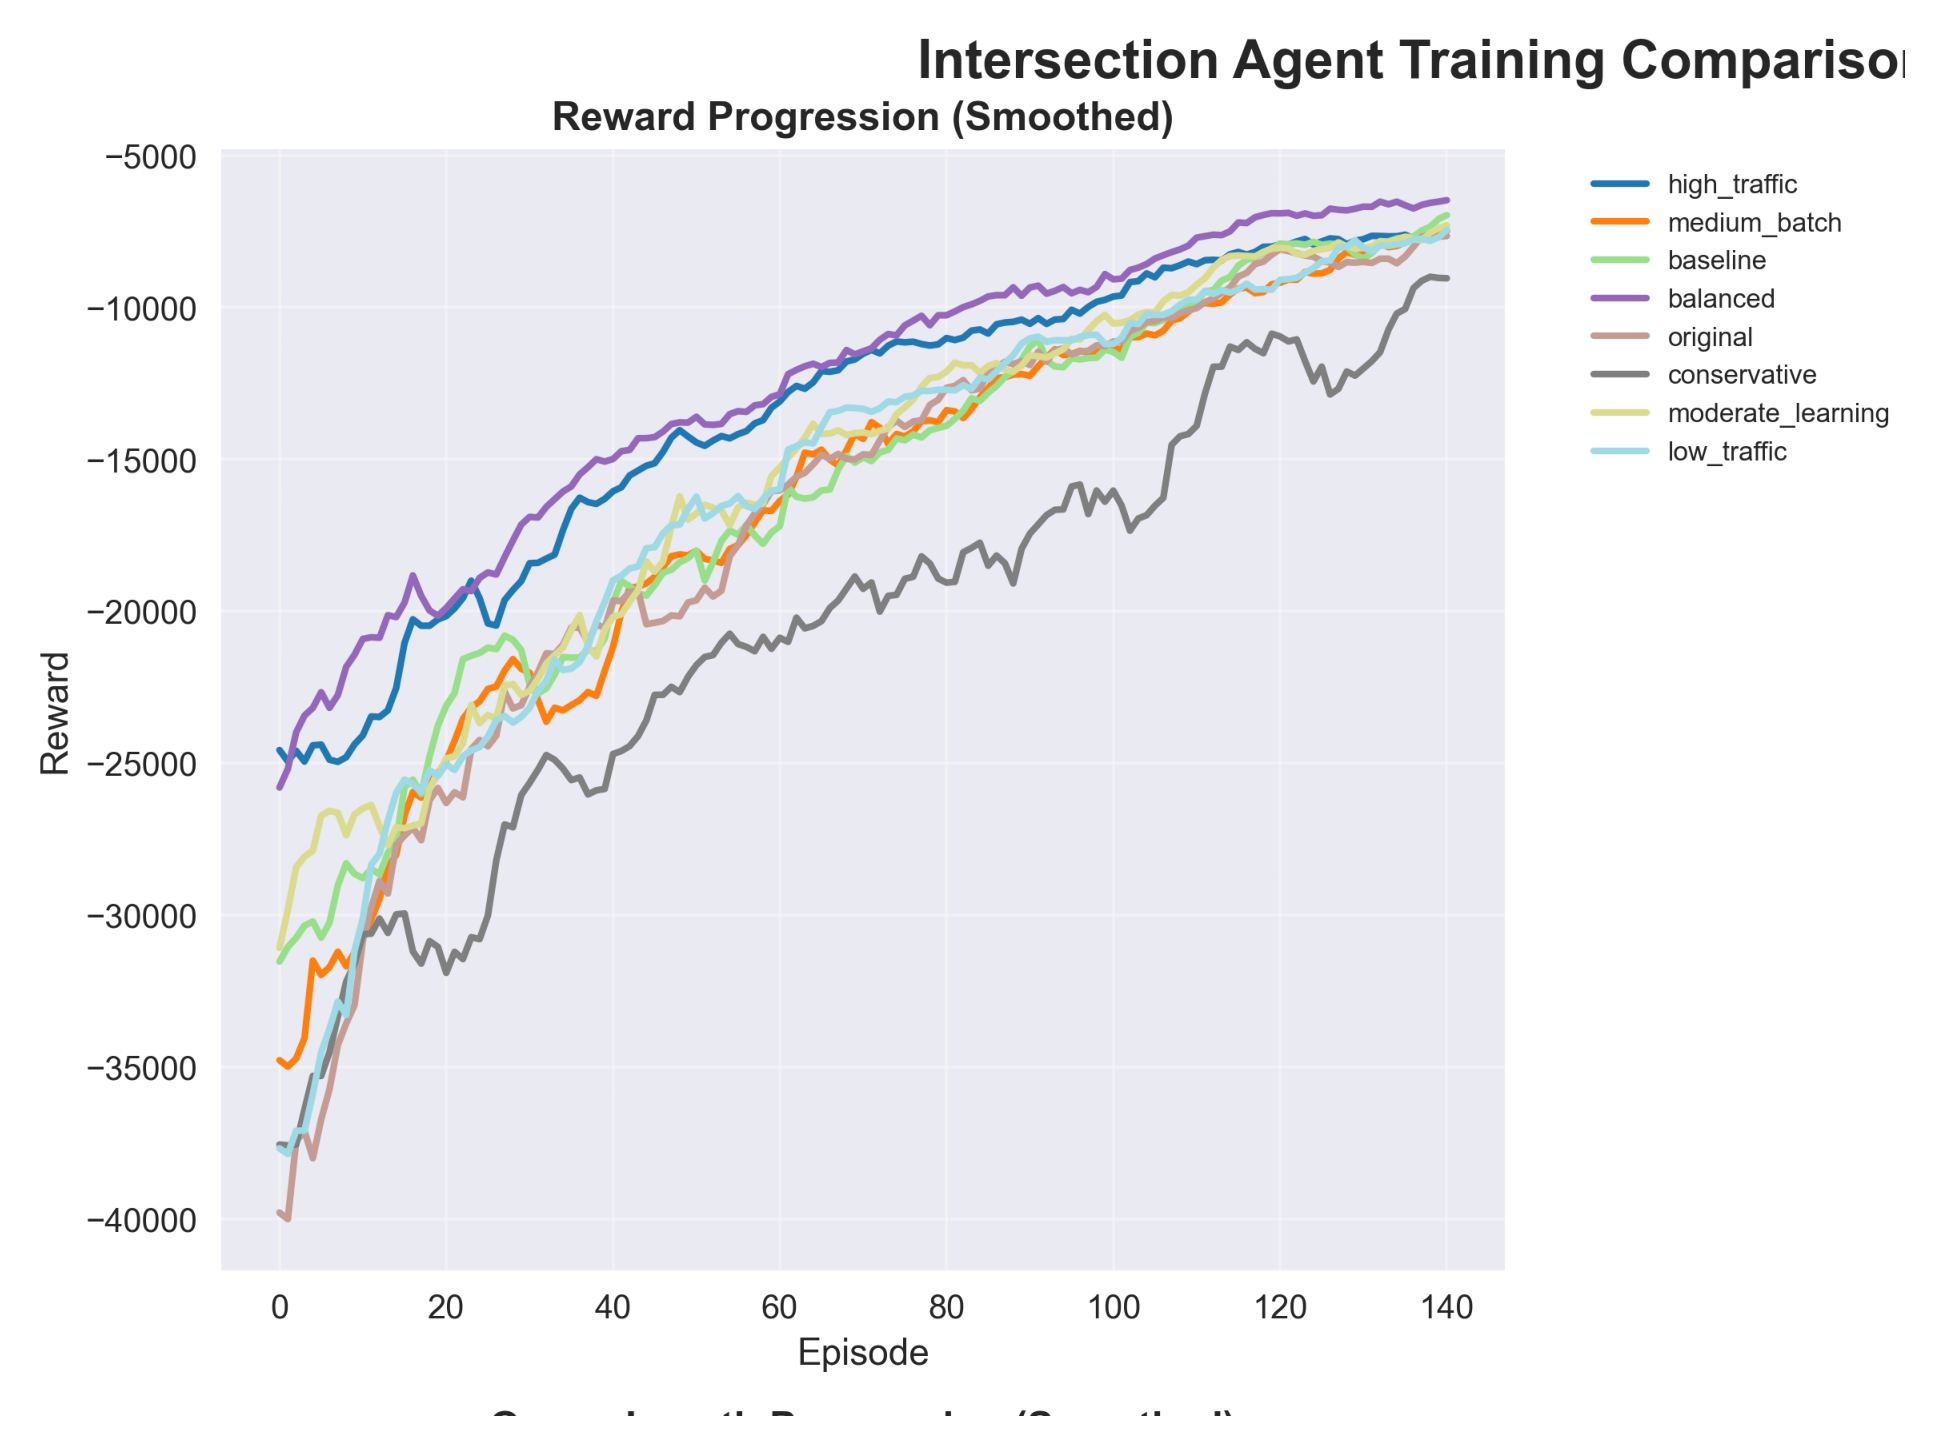
\includegraphics[width=\textwidth]{figures/individual_plots/intersection_filtered_reward_progress.png}
    \caption{Tiến trình phần thưởng của các mô hình intersection agent qua các tập huấn luyện (loại bỏ giá trị ngoại lai)}
    \label{fig:intersection_filtered_reward_progress}
\end{figure*}

Từ biểu đồ này, ta có thể phân tích chi tiết quá trình học của 8 mô hình có hiệu suất khả thi:

\begin{itemize}
    \item \textbf{Mô hình Balanced (màu xanh lam):} Cho thấy quá trình hội tụ ổn định nhất với độ dốc gradient ít dao động, đạt phần thưởng cuối -12.860. Mô hình bắt đầu học nhanh trong 50 episode đầu, sau đó ổn định.
    
    \item \textbf{Mô hình High Traffic (màu cam):} Có hiệu suất gần tương tự Balanced với phần thưởng -13,689, nhưng biến động nhiều hơn trong giai đoạn 100-150 episodes.
    
    \item \textbf{Nhóm trung bình (Moderate Learning, Baseline):} Có xu hướng học chậm hơn và đạt plateau sớm quanh episode 120-130, với mức độ hội tụ thấp hơn 15-20\% so với nhóm tốt nhất.
    
    \item \textbf{Mô hình Conservative (màu tím):} Cho thấy learning curve phẳng nhất, học rất chậm do learning rate thấp (0,0001), đạt phần thưởng chỉ -20.723.
\end{itemize}

Đặc biệt, biểu đồ cho thấy rõ tương quan giữa learning rate và tốc độ hội tụ: các mô hình với learning rate 0,0007-0,001 hội tụ nhanh và ổn định, trong khi learning rate quá thấp (<0,0005) dẫn đến học chậm.

\subsubsection{Thời gian chờ đợi trung bình}
Metric thời gian chờ đợi phản ánh trực tiếp hiệu quả của hệ thống trong việc giảm thiểu ùn tắc giao thông. Hình \ref{fig:intersection_filtered_waiting_time} so sánh hiệu suất của các mô hình theo chỉ số này.

\begin{figure*}[!htp]
    \centering
    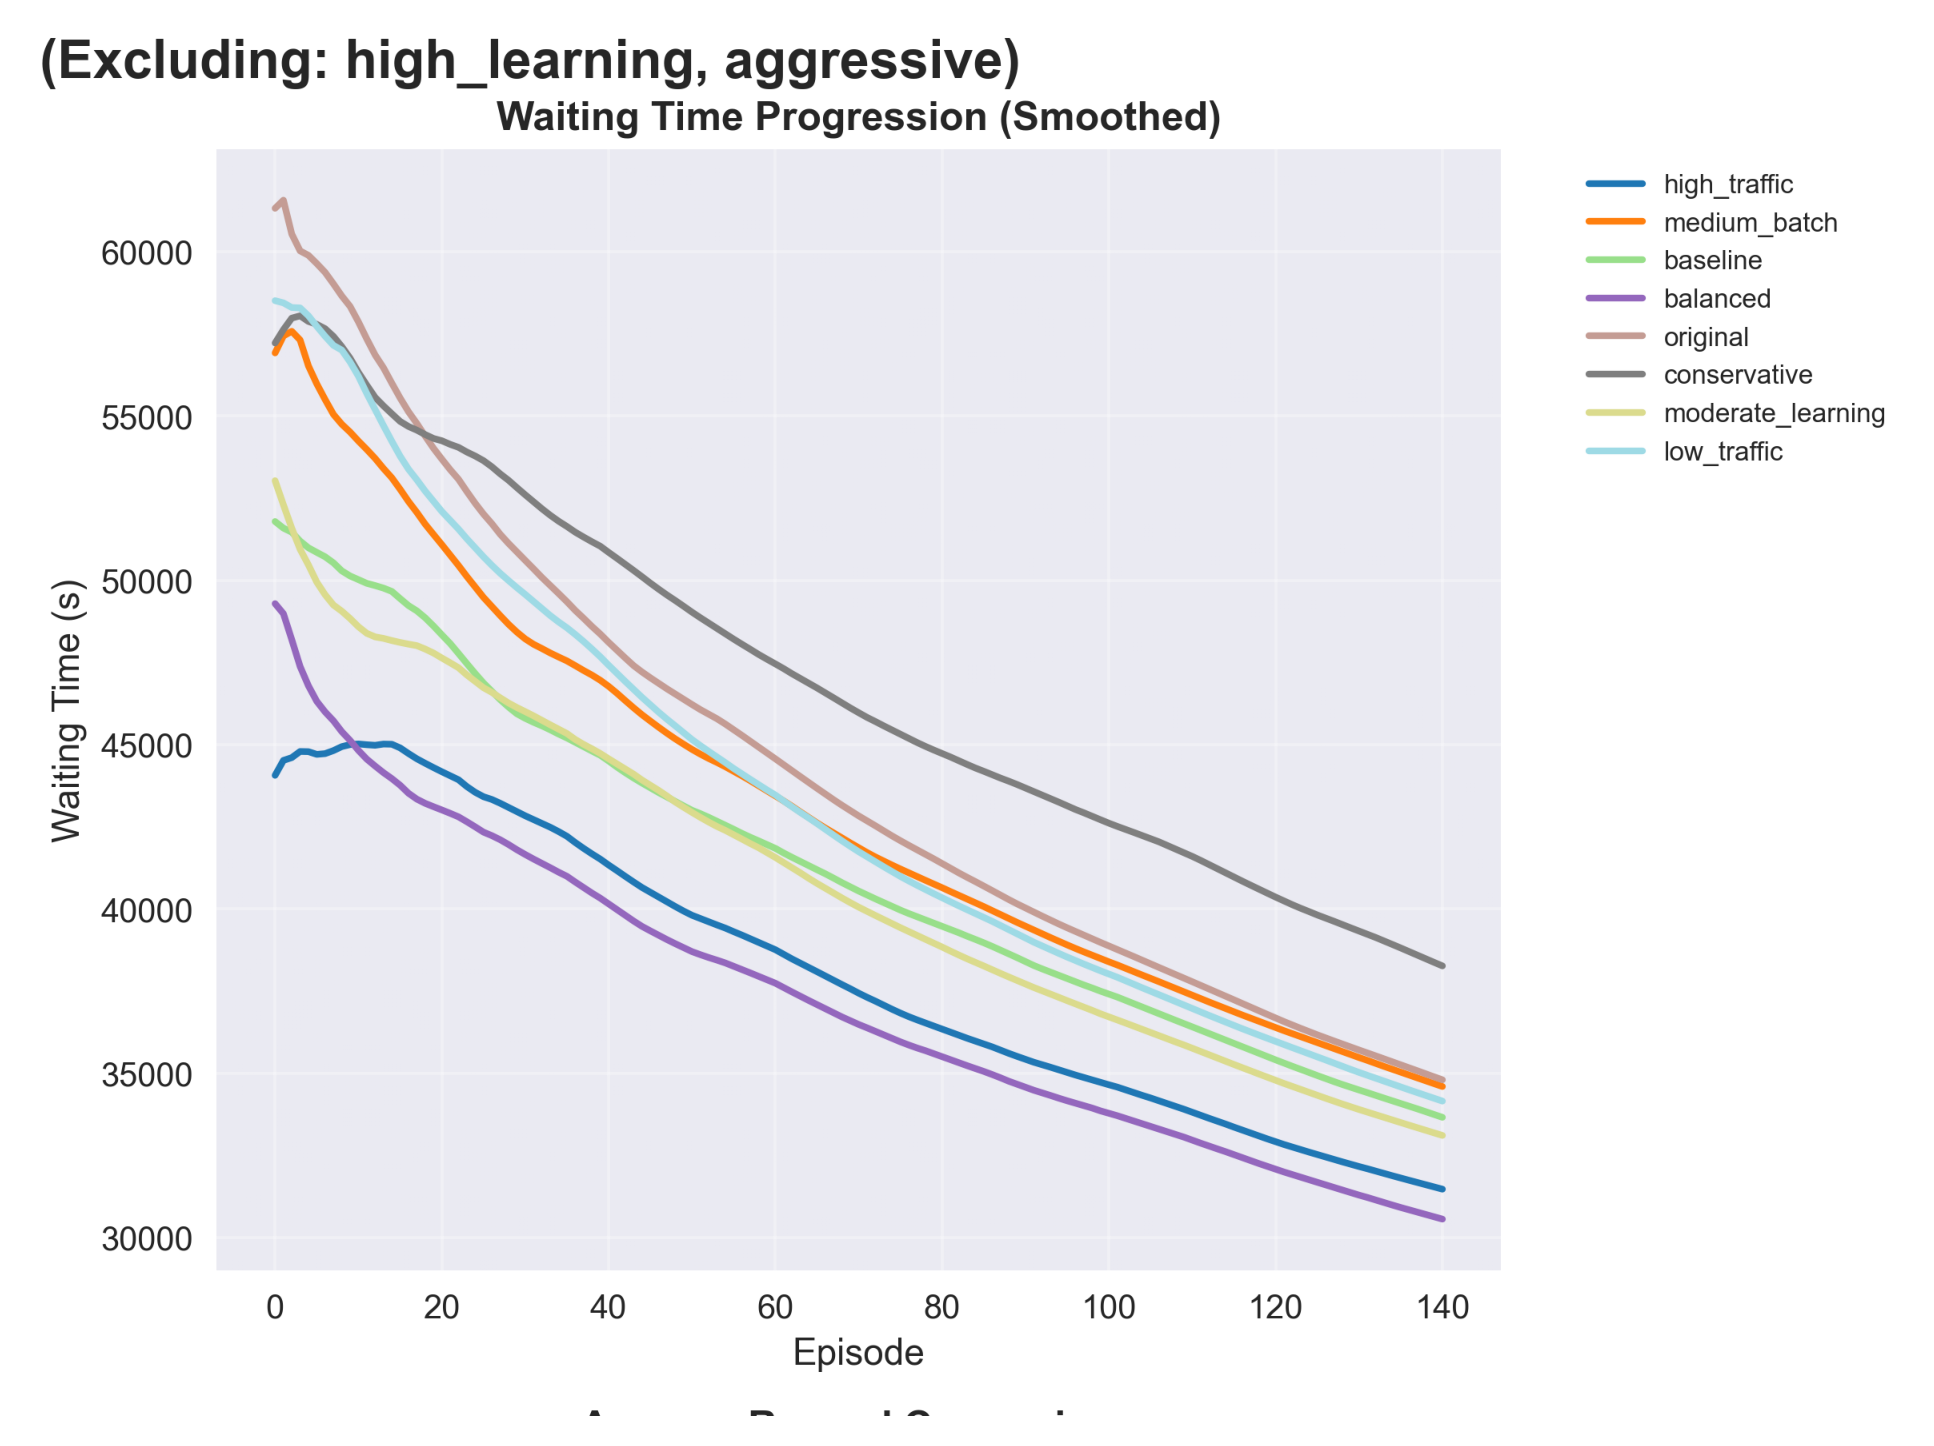
\includegraphics[width=0.7\textwidth]{figures/individual_plots/intersection_filtered_waiting_time.png}
    \caption{So sánh thời gian chờ đợi trung bình của các mô hình intersection agent}
    \label{fig:intersection_filtered_waiting_time}
\end{figure*}

Kết quả phân tích cho thấy mô hình Balanced đạt thời gian chờ thấp nhất (37,5s), vượt trội so với các mô hình khác và chứng minh hiệu quả của việc cân bằng các siêu tham số (hyperparameter).

\subsubsection{Độ dài hàng đợi trung bình}
Độ dài hàng đợi là một chỉ số quan trọng khác để đánh giá mức độ ùn tắc tại giao lộ. Hình \ref{fig:intersection_filtered_queue_length} thể hiện sự so sánh giữa các mô hình dựa trên metric này.

\begin{figure*}[!htp]
    \centering
    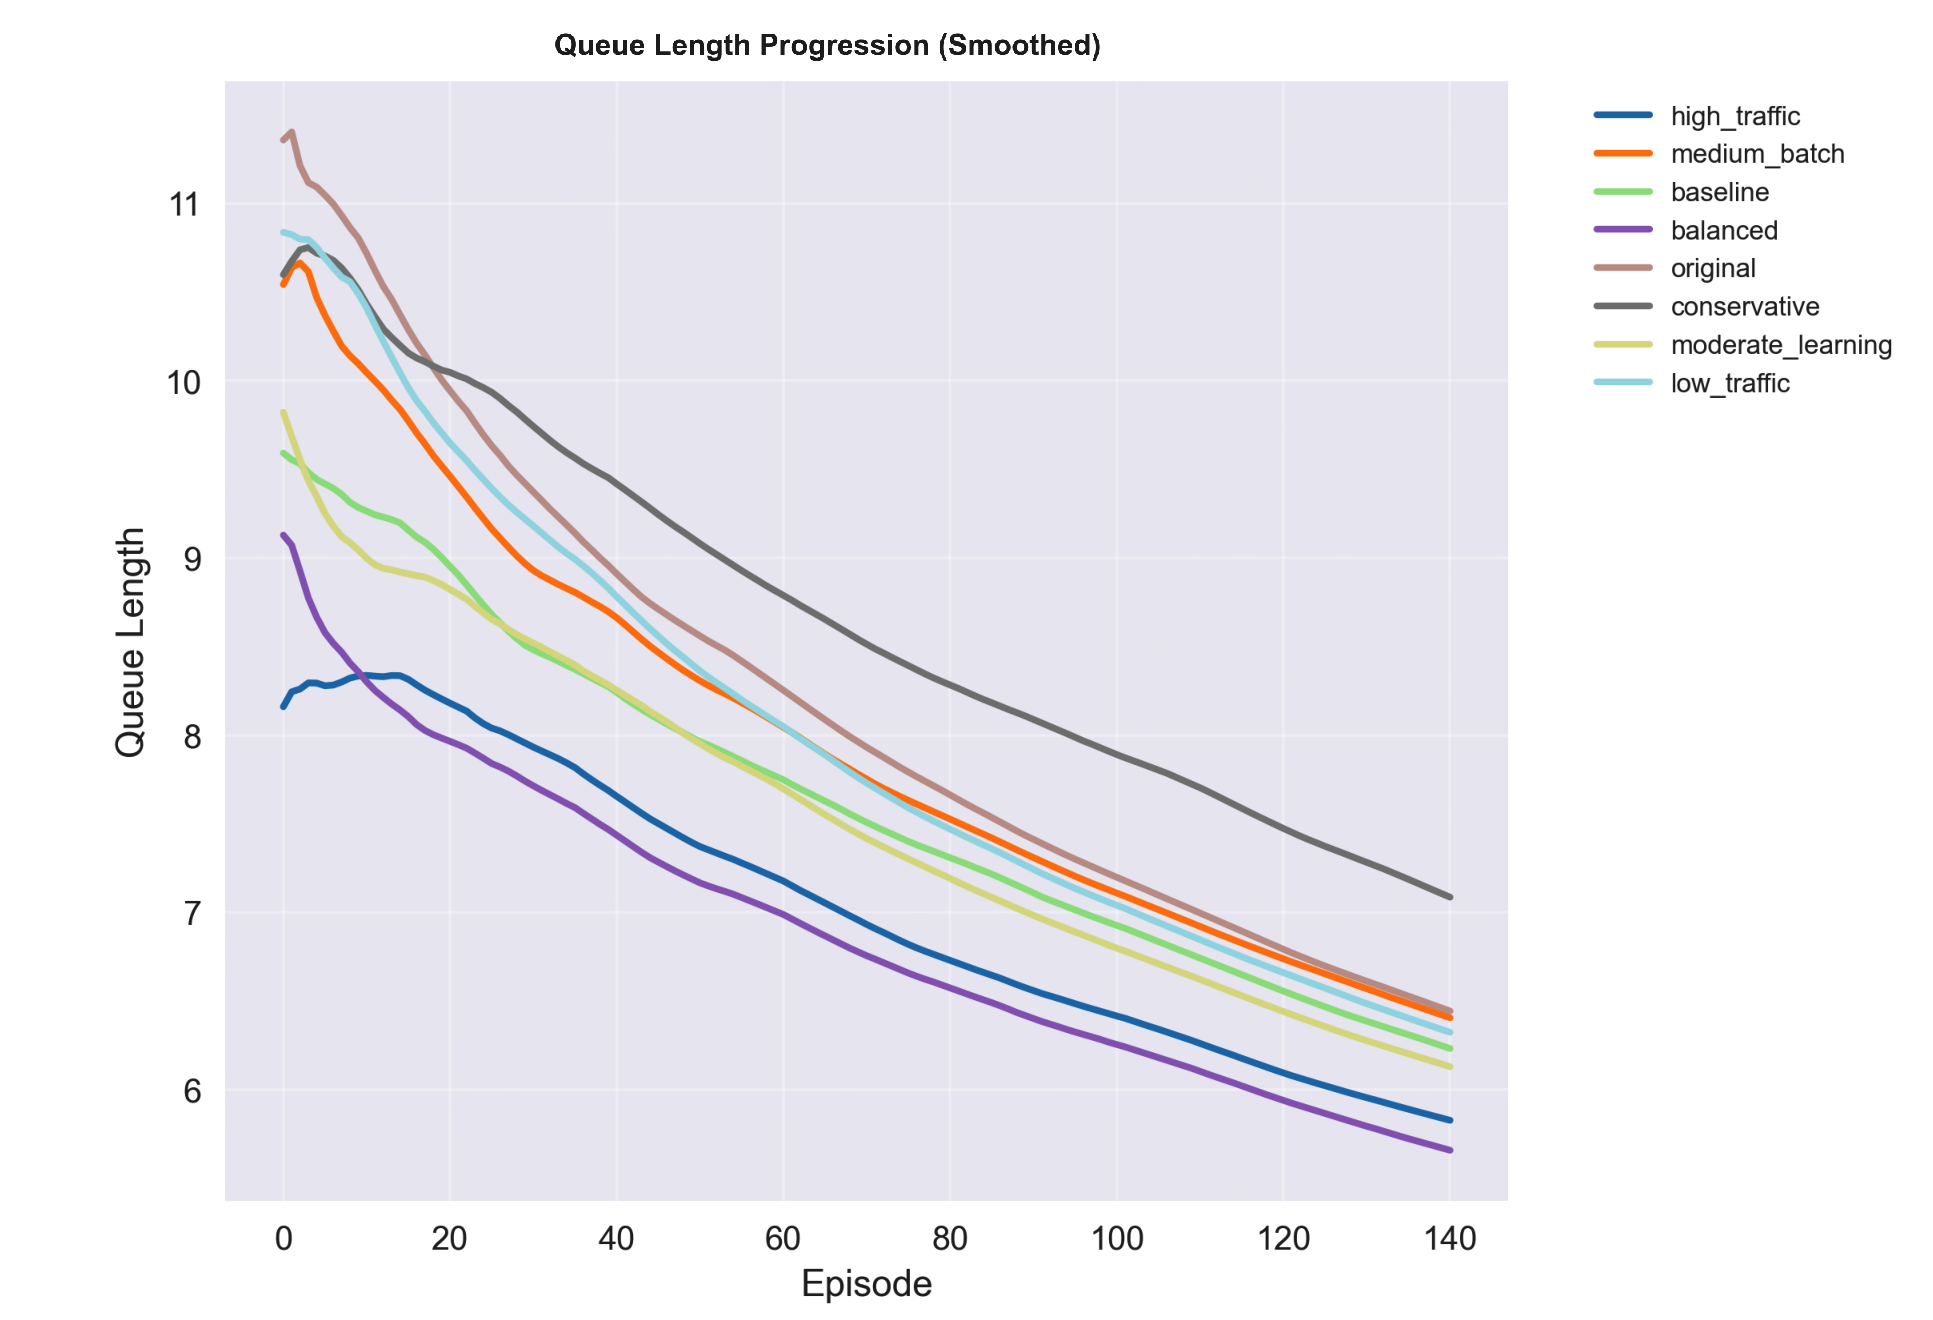
\includegraphics[width=0.7\textwidth]{figures/individual_plots/intersection_filtered_queue_length.png}
    \caption{So sánh độ dài hàng đợi trung bình của các mô hình intersection agent}
    \label{fig:intersection_filtered_queue_length}
\end{figure*}

Kết quả đánh giá cho thấy mô hình Balanced cũng đạt độ dài hàng đợi nhỏ nhất (6,95 xe), tương quan trực tiếp với hiệu suất thời gian chờ đợi.

\subsubsection{So sánh tổng thể hiệu suất}
Để có cái nhìn tổng quan về hiệu suất của tất cả các mô hình, nghiên cứu tổng hợp ba chỉ số chính trong một biểu đồ thống nhất. Hình \ref{fig:intersection_filtered_performance_summary} cung cấp phân tích so sánh đa chiều.

\begin{figure}[!htp]
    \centering
    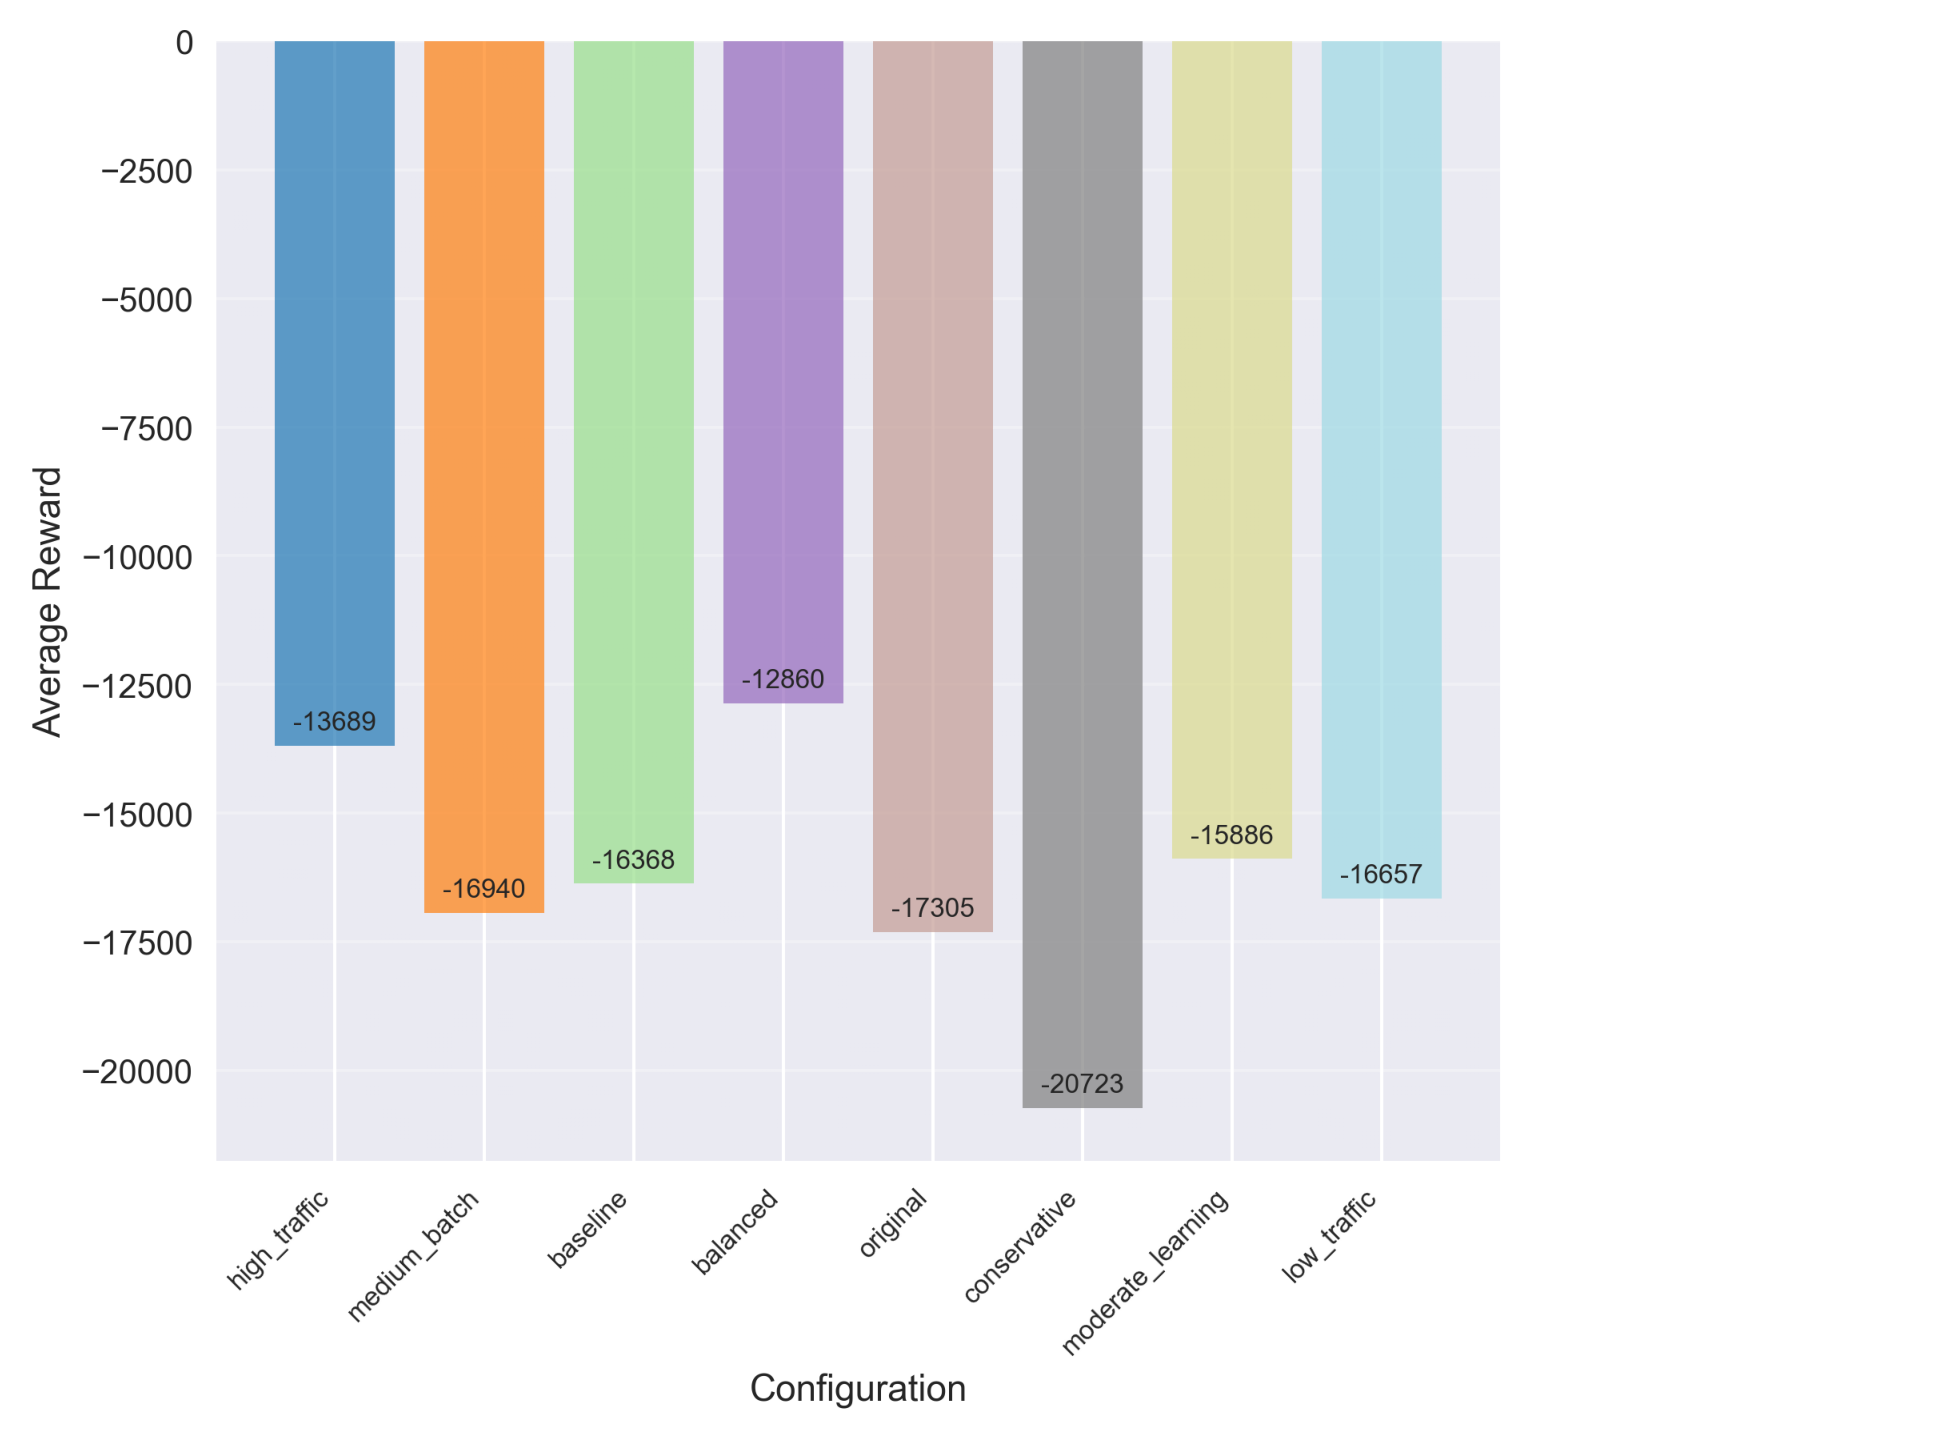
\includegraphics[width=\textwidth]{
        figures/individual_plots/intersection_filtered_performance_summary.png
    }
    \caption{Tổng hợp so sánh hiệu suất các mô hình intersection agent}
    \label{fig:intersection_filtered_performance_summary}
\end{figure}

Biểu đồ tổng hợp này cho phép so sánh trực tiếp hiệu suất của các mô hình dựa trên ba chỉ số chính:

\begin{itemize}
    \item \textbf{Phân bố hiệu suất:} Biểu đồ thể hiện rõ sự phân tầng hiệu suất với 3 nhóm rõ rệt - nhóm cao (Balanced, High Traffic), nhóm trung bình (5 mô hình), và nhóm thấp (Conservative).
    
    \item \textbf{Tương quan chỉ số:} Có sự tương quan mạnh giữa ba chỉ số - mô hình có phần thưởng cao thường có thời gian chờ đợi và độ dài hàng đợi thấp, chứng minh tính nhất quán của phương pháp đánh giá.
    
    \item \textbf{Margin of superiority:} Balanced vượt trội với margin đáng kể - thấp hơn 9\% về thời gian chờ và 8,5\% về độ dài hàng đợi so với mô hình tốt thứ hai (High Traffic).
    
    \item \textbf{Ngưỡng khả thi:} Các mô hình có thời gian chờ đợi trung bình < 45s và độ dài hàng đợi trung bình < 8,5 xe được xem là khả thi cho triển khai thực tế dựa trên tiêu chuẩn giao thông đô thị.
\end{itemize}

Kết quả khẳng định sự vượt trội toàn diện của mô hình Balanced, không chỉ về một metric đơn lẻ mà trên toàn bộ phổ đánh giá hiệu suất.

\subsection{So sánh đầy đủ bao gồm giá trị ngoại lai}

Để thể hiện tác động nghiêm trọng của việc lựa chọn siêu tham số không phù hợp,
nghiên cứu cũng trình bày kết quả đầy đủ của tất cả 10 mô hình bao gồm cả hai mô
hình có hiệu suất cực kém.

\subsubsection{Tiến trình reward với giá trị ngoại lai}
Để hiểu rõ tác động của việc lựa chọn siêu tham số không phù hợp, nghiên cứu trình bày kết quả đầy đủ bao gồm cả các mô hình thất bại. Hình \ref{fig:intersection_full_reward_progress} cho thấy sự tương phản rõ rệt giữa các nhóm mô hình.

\begin{figure}[!htp]
    \centering
    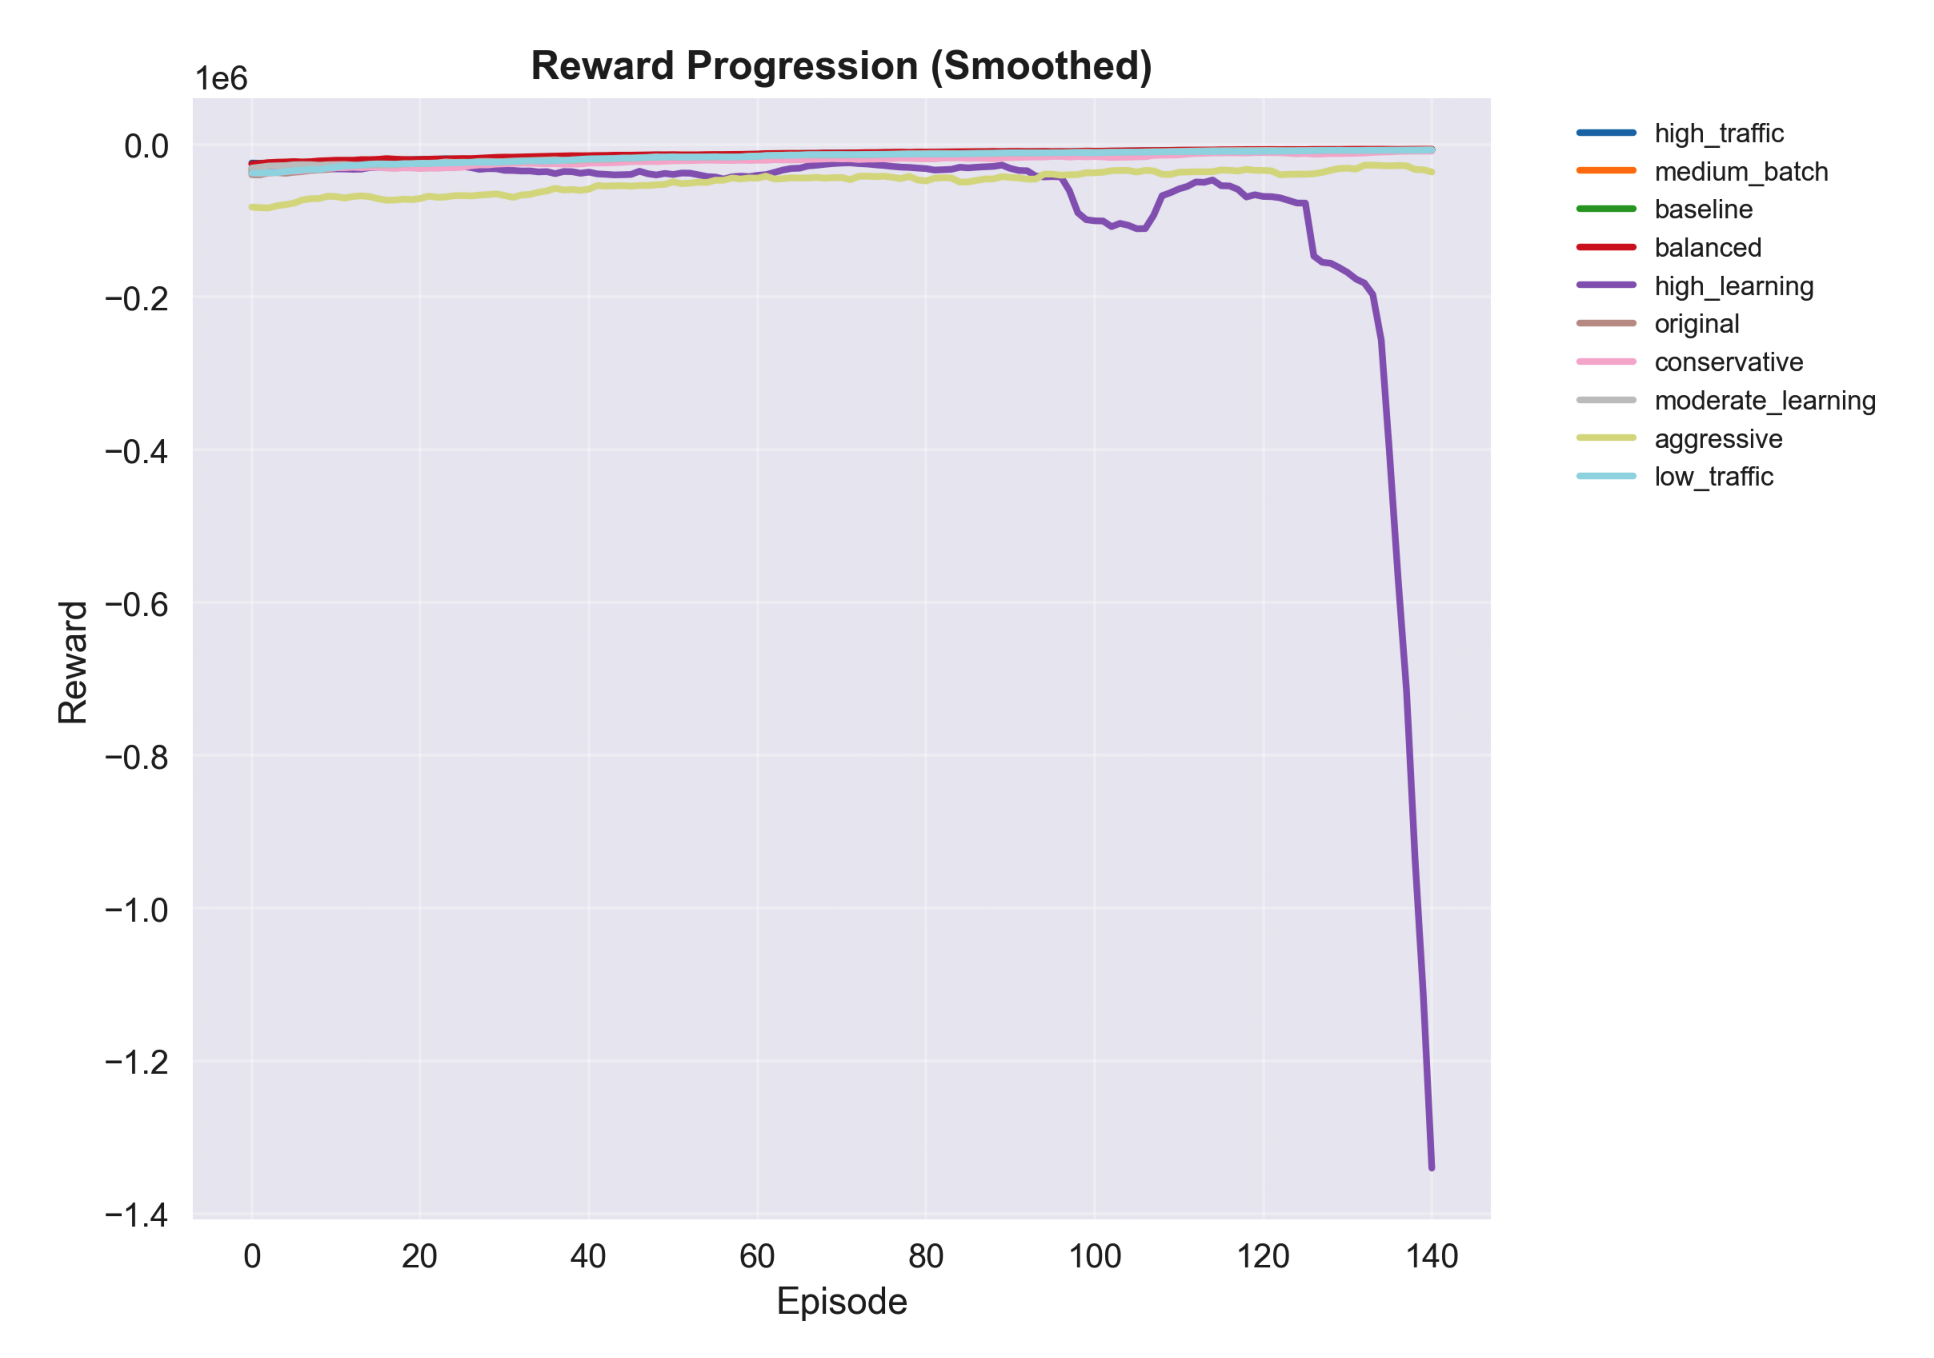
\includegraphics[width=\textwidth]{
        figures/individual_plots/intersection_full_reward_progress.png
    }
    \caption{Tiến trình phần thưởng của tất cả 10 mô hình intersection agent bao gồm giá trị ngoại lai}
    \label{fig:intersection_full_reward_progress}
\end{figure}

Biểu đồ này cho thấy rõ ràng sự khác biệt lớn giữa các mô hình, với High Learning có hiệu suất cực kỳ kém (phần thưởng -138.191) và Aggressive cũng thất bại hoàn toàn (-50.135).

\subsubsection{Thời gian chờ đợi với giá trị ngoại lai}
Metric thời gian chờ đợi khi bao gồm các mô hình thất bại cho thấy mức độ ảnh hưởng của việc cấu hình tham số không phù hợp. Hình \ref{fig:intersection_full_waiting_time} minh họa rõ ràng sự khác biệt lớn này.

\begin{figure}[!htp]
    \centering
    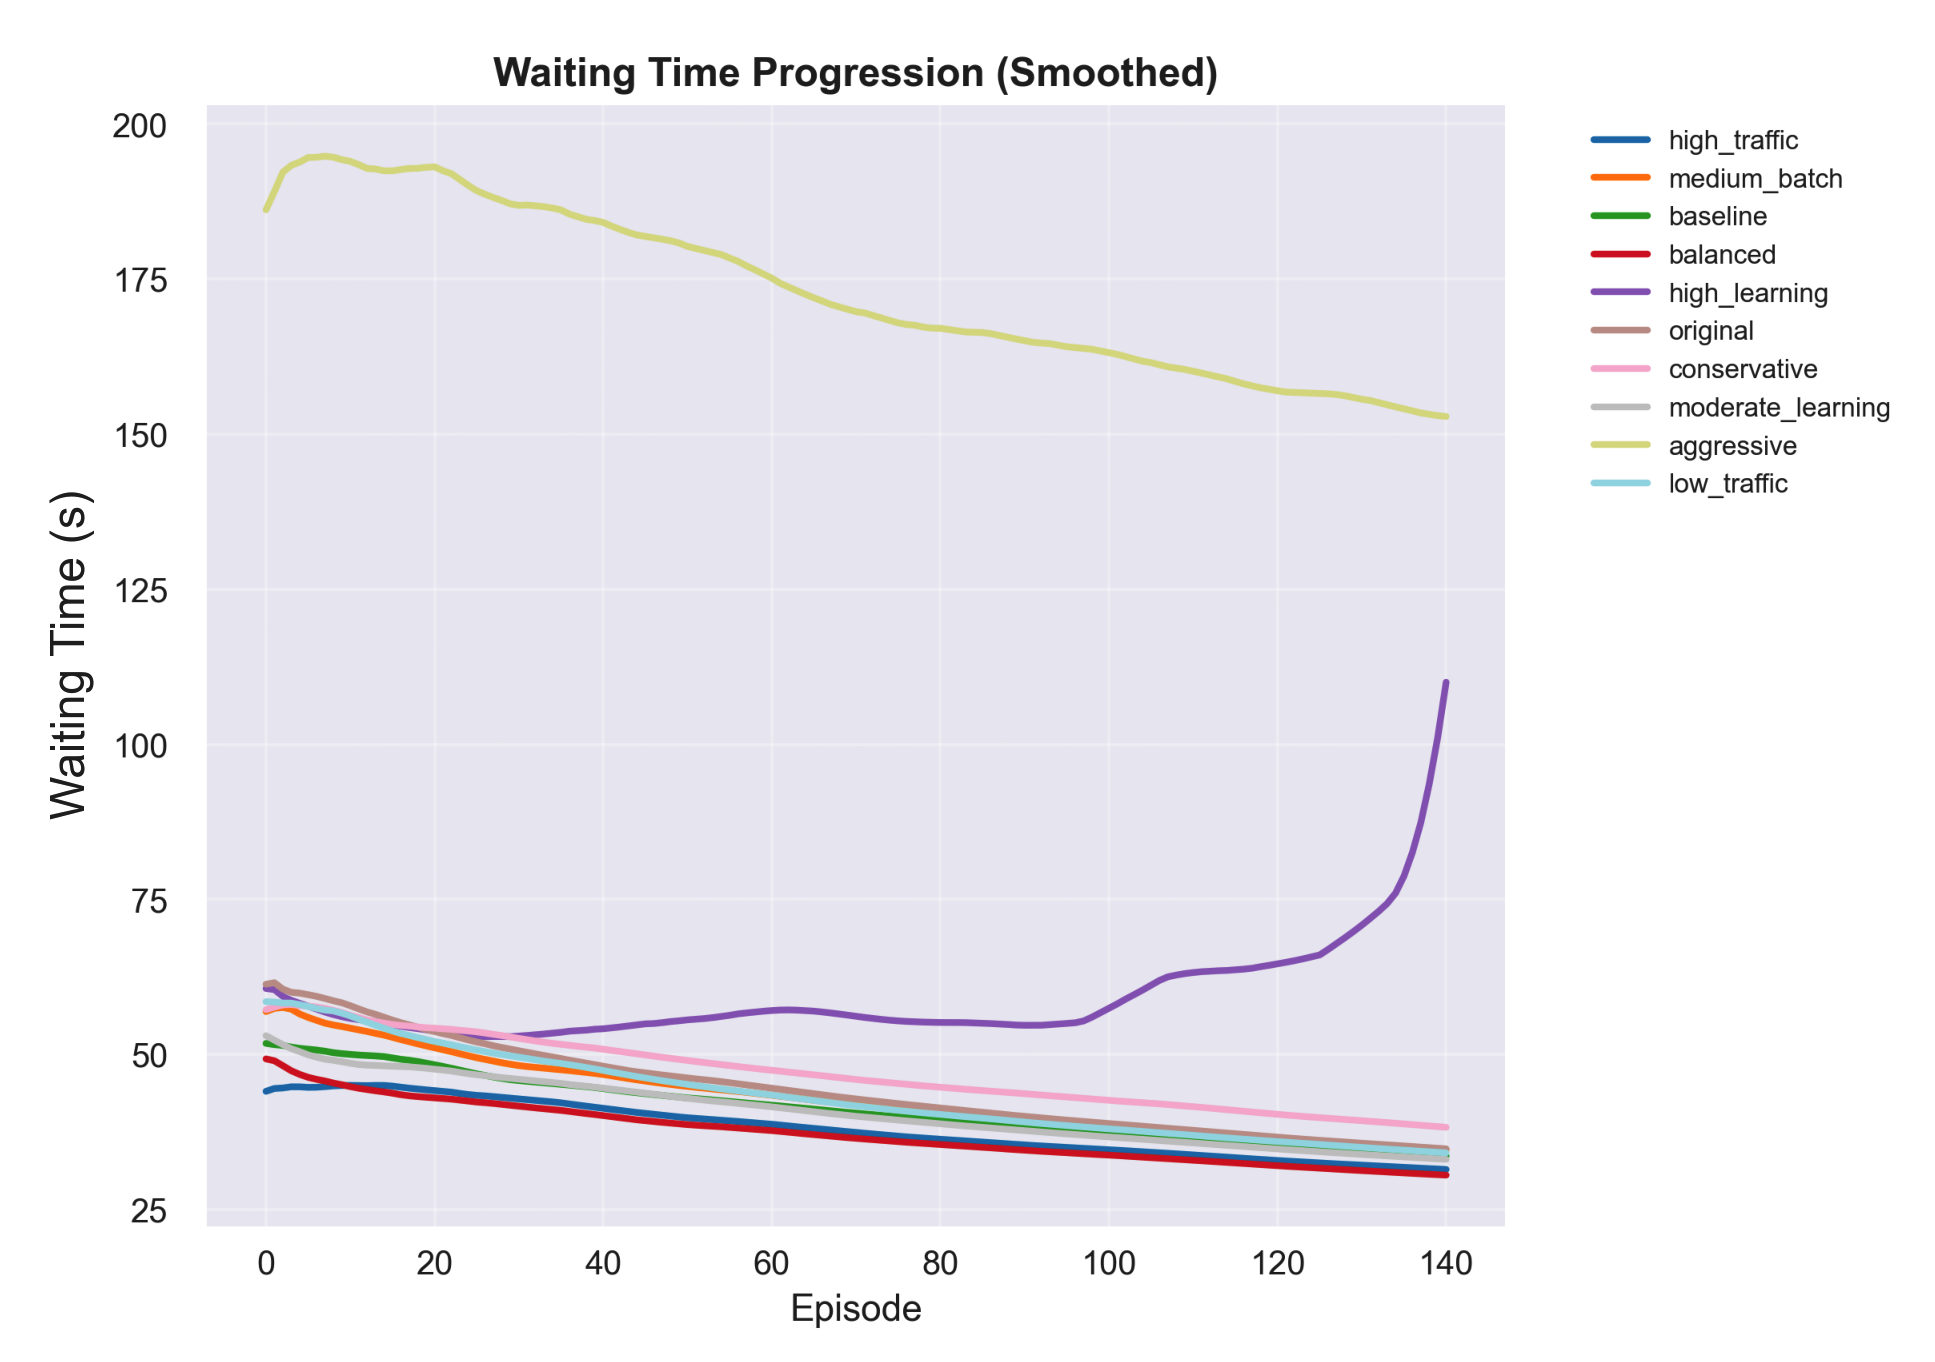
\includegraphics[width=\textwidth]{
        figures/individual_plots/intersection_full_waiting_time.png
    }
    \caption{So sánh thời gian chờ đợi của tất cả 10 mô hình bao gồm giá trị ngoại lai}
    \label{fig:intersection_full_waiting_time}
\end{figure}

Kết quả phân tích thể hiện tác động trực tiếp của siêu tham số không phù hợp lên hiệu suất thực tế, với mô hình Aggressive gây ra thời gian chờ cực lớn (172,7s) - gấp 4,6 lần so với mô hình Balanced.

\subsubsection{Độ dài hàng đợi với giá trị ngoại lai}
Tương tự như thời gian chờ đợi, độ dài hàng đợi cũng bị ảnh hưởng nghiêm trọng bởi việc lựa chọn tham số không phù hợp. Hình \ref{fig:intersection_full_queue_length} thể hiện sự chênh lệch đáng kể giữa các mô hình.

\begin{figure}[!htp]
    \centering
    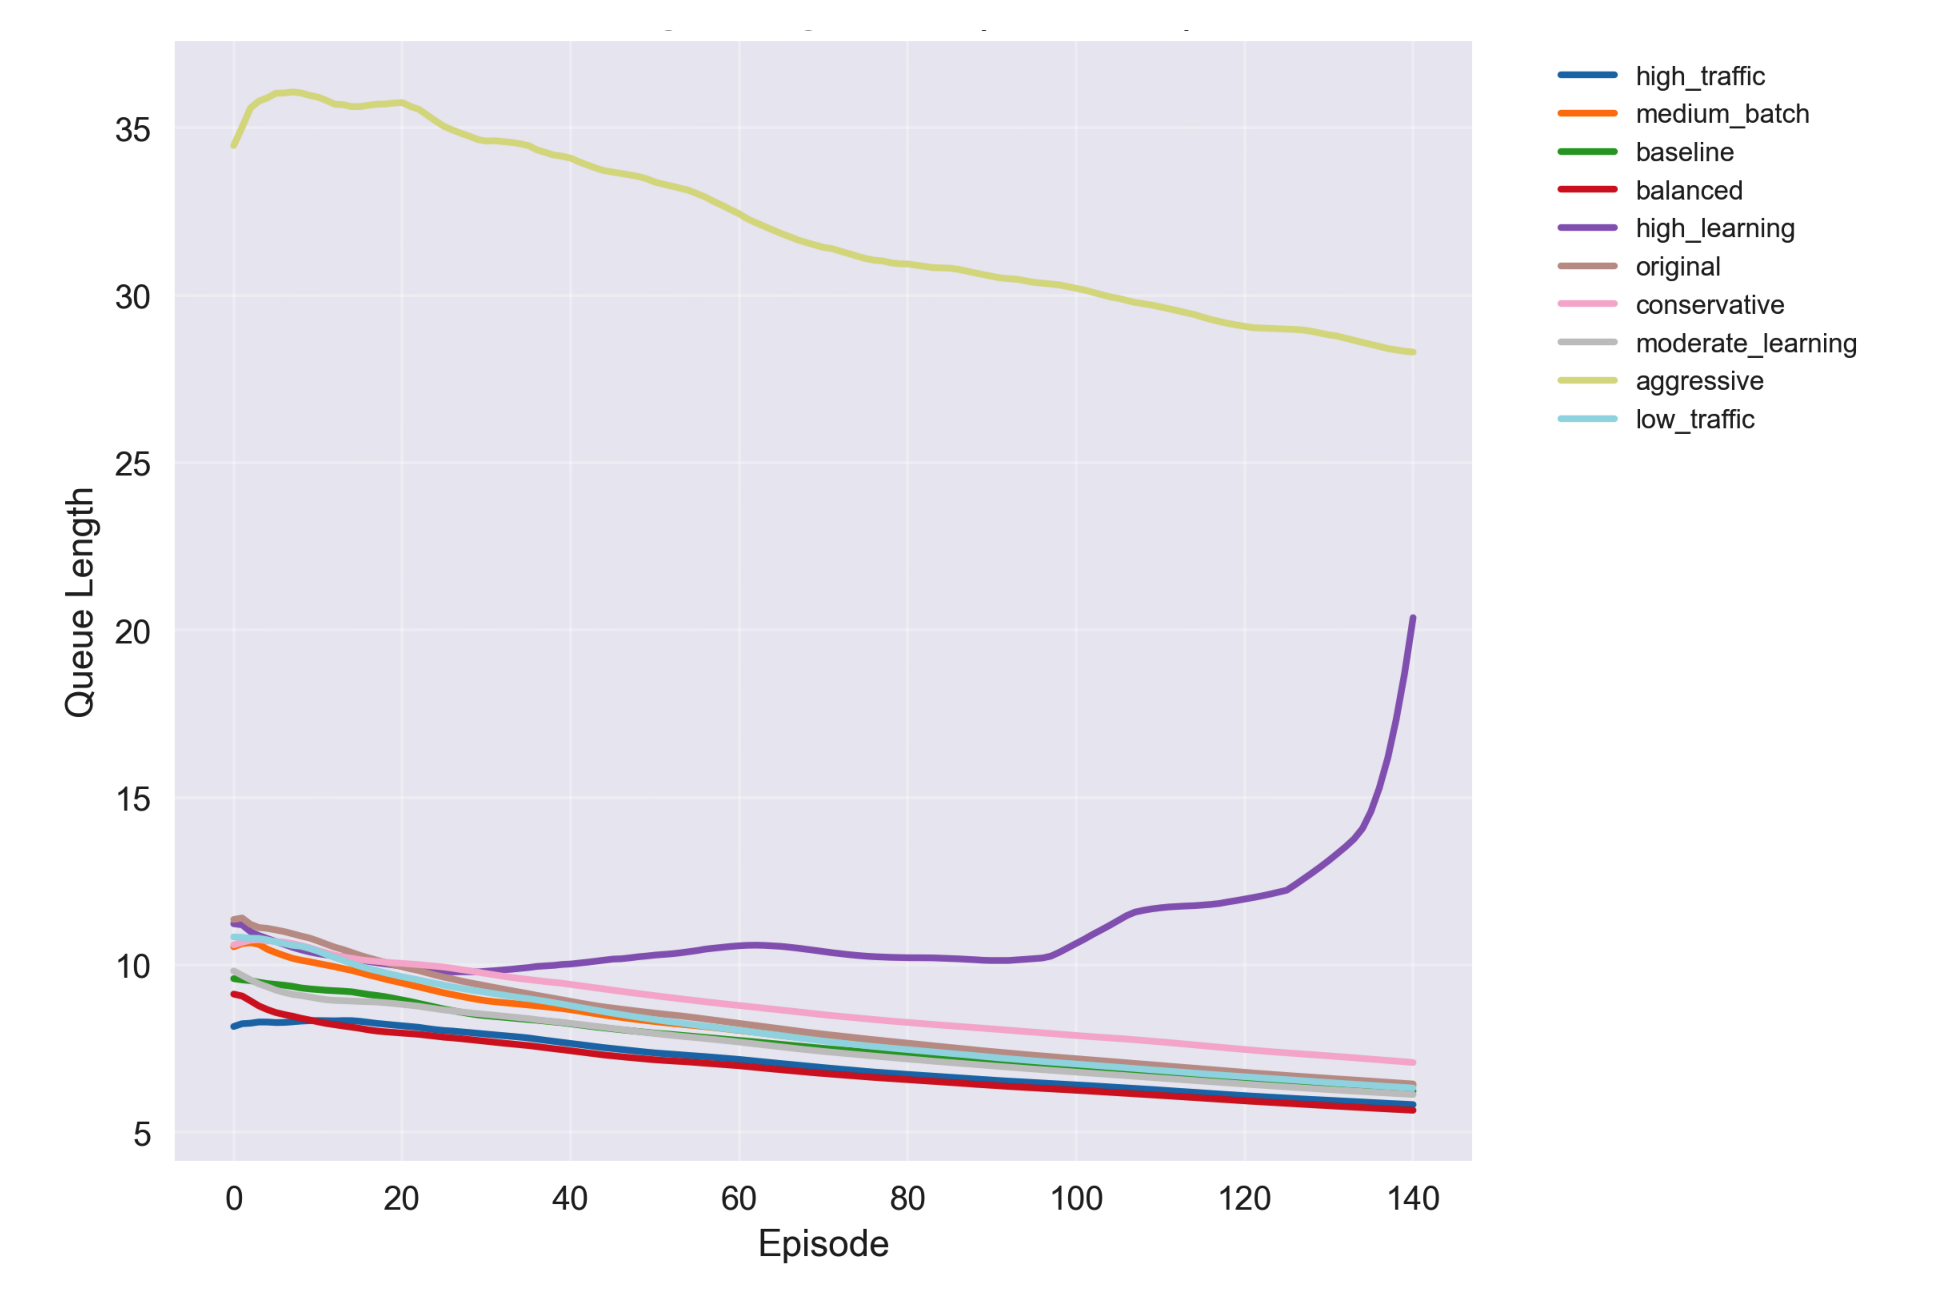
\includegraphics[width=\textwidth]{
        figures/individual_plots/intersection_full_queue_length.png
    }
    \caption{So sánh độ dài hàng đợi của tất cả 10 mô hình bao gồm giá trị ngoại lai}
    \label{fig:intersection_full_queue_length}
\end{figure}

Dữ liệu cho thấy mô hình Aggressive tạo ra hàng đợi dài nhất (31,98 xe) - gấp 4,6 lần so với Balanced, chứng minh tác động nghiêm trọng của việc lựa chọn tham số không phù hợp.

\subsubsection{Tổng hợp so sánh với giá trị ngoại lai}
Biểu đồ tổng hợp đầy đủ cho thấy phạm vi biến động hiệu suất rộng lớn giữa các mô hình. Hình \ref{fig:intersection_full_performance_summary} cung cấp cái nhìn toàn diện về tác động của việc điều chỉnh tham số.

\begin{figure}[!htp]
    \centering
    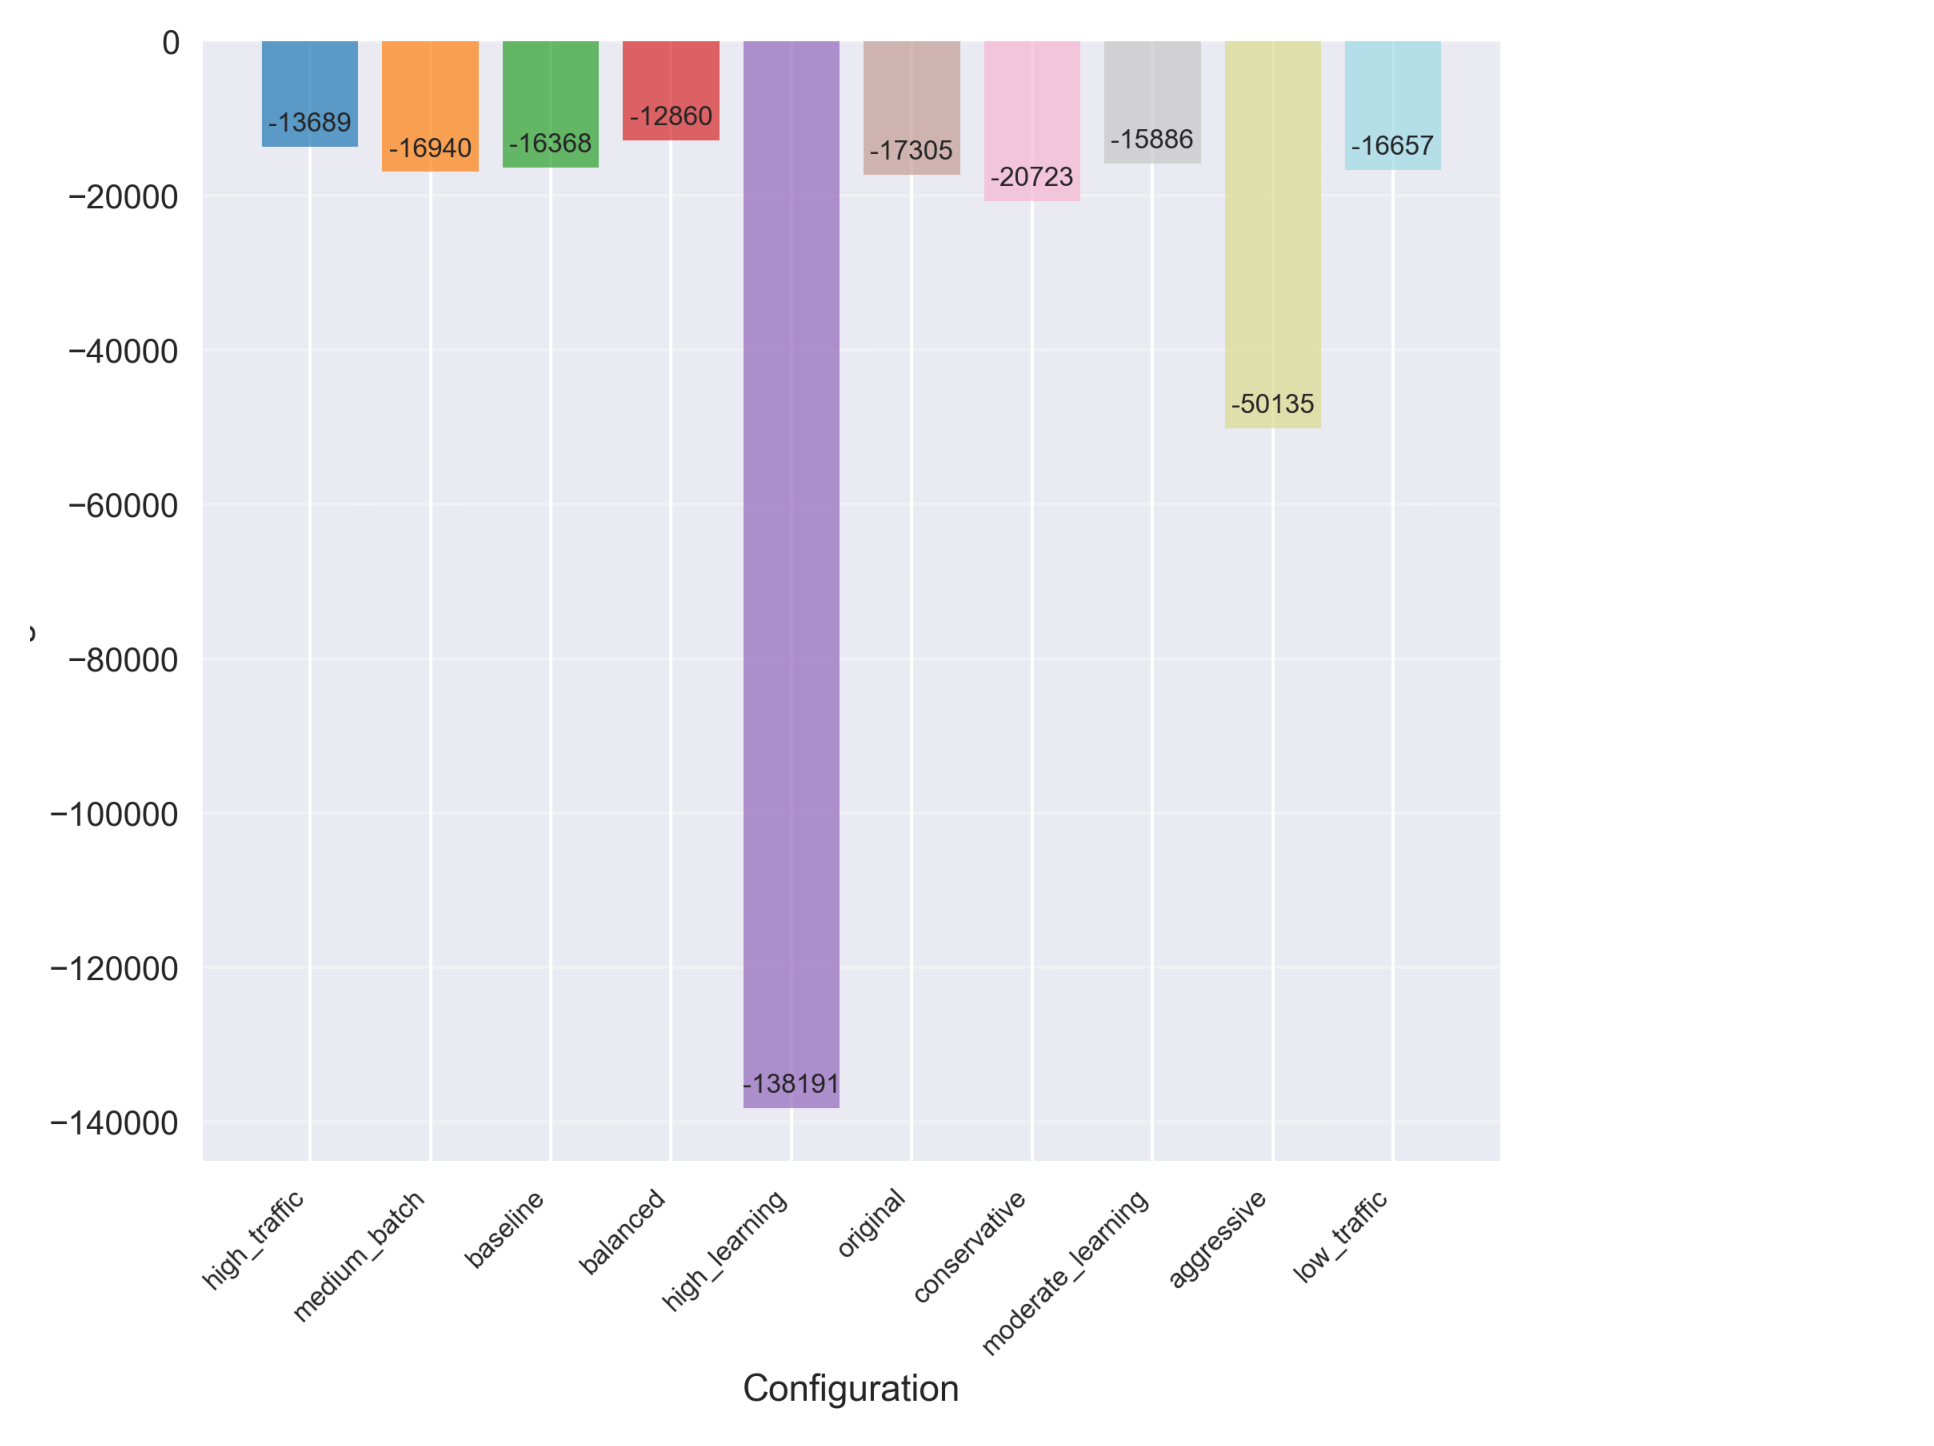
\includegraphics[width=\textwidth]{
        figures/individual_plots/intersection_full_performance_summary.png
    }
    \caption{Tổng hợp so sánh hiệu suất tất cả 10 mô hình intersection agent}
    \label{fig:intersection_full_performance_summary}
\end{figure}

Biểu đồ tổng hợp này cho thấy rõ ràng sự thay đổi nghiêm trọng khi lựa chọn tham số không phù hợp: mô hình Aggressive đạt phần thưởng -50.135 (kém 290\% so với Balanced), trong khi High Learning đạt -138.191 (kém 975\% so với Balanced). Điều này nhấn mạnh tầm quan trọng của việc lựa chọn siêu tham số cẩn thận trong Deep Reinforcement Learning.
\newpage
\subsection{Hiệu suất của mô hình tối ưu}

Mô hình \textbf{Balanced} thể hiện hiệu suất vượt trội với các chỉ số sau:

\begin{align}
    \text{Phần thưởng trung bình}     & : -12.860             \\
    \text{Thời gian chờ trung bình}   & : 37,5 \text{ giây} \\
    \text{Độ dài hàng đợi trung bình} & : 6,95 \text{ xe}
\end{align}

Kết quả này cho thấy mô hình Balanced không chỉ đạt được hiệu suất cao mà còn duy
trì sự ổn định trong suốt quá trình hoạt động.

\subsection{So sánh tổng thể giao lộ đơn}

Bảng dưới đây tổng hợp kết quả so sánh hiệu suất của tất cả các mô hình, được sắp
xếp theo thứ tự từ tốt nhất đến kém nhất:

\begin{table*}[!htp]
    \centering
    \caption{Kết quả so sánh hiệu suất các mô hình DQN với phân tích nhóm}
    \label{tab:model_performance_comparison}
    \footnotesize
    \begin{tabular}{|l|c|c|c|l|}
        \hline 
        \textbf{Mô hình}  & \textbf{Phần thưởng TB} & \textbf{Thời gian chờ TB (s)} & \textbf{Độ dài hàng đợi TB} & \textbf{Nhóm hiệu suất} \\
        \hline 
        \multicolumn{5}{|c|}{\textbf{NHÓM HIỆU SUẤT CAO (Top 25\%)}} \\
        \hline
        \textbf{Balanced (tốt nhất)} & \textbf{-12.860}     & \textbf{37,5}            & \textbf{6,95}               & Tối ưu \\
        \hline
        High Traffic               & -13.689              & 38,0                     & 7,04                        & Khả thi \\
        \hline
        \multicolumn{5}{|c|}{\textbf{NHÓM HIỆU SUẤT TRUNG BÌNH (25-75\%)}} \\
        \hline
        Moderate Learning          & -15.886              & 41,0                     & 7,59                        & Chấp nhận được \\
        \hline
        Baseline                   & -16.368              & 41,4                     & 7,67                        & Chấp nhận được \\
        \hline
        Low Traffic                & -16.657              & 43,6                     & 8,07                        & Chấp nhận được \\
        \hline
        Medium Batch               & -16.940              & 43,3                     & 8,02                        & Chấp nhận được \\
        \hline
        Original                   & -17.305              & 44,7                     & 8,28                        & Chấp nhận được \\
        \hline
        Conservative               & -20.723              & 47,0                     & 8,69                        & Thấp \\
        \hline
        \multicolumn{5}{|c|}{\textbf{NHÓM HIỆU SUẤT THẤP (Bottom 25\% - Outliers)}} \\
        \hline
        Aggressive                 & -50.135              & 172,7                    & 31,98                       & Thất bại \\
        \hline
        High Learning (tệ nhất)              & -138.191             & 61,5                     & 11,39                       & Thất bại hoàn toàn \\
        \hline
    \end{tabular}
\end{table*}

\subsection{Phân tích xu thế và nhóm hiệu suất}

Từ kết quả trong Bảng \ref{tab:model_performance_comparison}, có thể rút ra các xu thế quan trọng:

\subsubsection{Nhóm hiệu suất cao (Top 25\%)}
\begin{itemize}
    \item \textbf{Balanced}: Đạt hiệu suất tốt nhất với thời gian chờ 37,5s và hàng đợi 6,95 xe
    \item \textbf{High Traffic}: Xếp thứ 2 với hiệu suất sát sao (chênh lệch 1,3\% về thời gian chờ)
    \item \textbf{Đặc điểm chung}: Learning rate trung bình (0,0007-0,001), batch size hợp lý (64-128)
\end{itemize}

\subsubsection{Nhóm hiệu suất trung bình (25-75\%)}
\begin{itemize}
    \item \textbf{Xu thế}: Thời gian chờ dao động 41-47s, hàng đợi 7,6-8,7 xe
    \item \textbf{Chênh lệch với nhóm cao}: 9-25\% về thời gian chờ đợi
    \item \textbf{Nguyên nhân}: Learning rate quá thấp (Conservative) hoặc cấu hình không tối ưu
\end{itemize}

\subsubsection{Nhóm hiệu suất thấp (Bottom 25\% - Outliers)}
\begin{itemize}
    \item \textbf{Aggressive}: Thời gian chờ 172,7s - gấp 4,6 lần so với mô hình tốt nhất
    \item \textbf{High Learning}: Phần thưởng -138.191 - gấp 10,7 lần độ lệch so với tốt nhất
    \item \textbf{Nguyên nhân}: Learning rate quá cao (0,005-0,01) gây instability
\end{itemize}

\subsubsection{Kết luận xu thế}
\begin{enumerate}
    \item \textbf{Learning rate tối ưu}: Khoảng 0,0007-0,001 cho hiệu suất cao
    \item \textbf{Batch size}: 64-128 tỏ ra hiệu quả nhất
    \item \textbf{Nguy cơ cao}: Learning rate > 0,003 gây training instability nghiêm trọng
    \item \textbf{Tính ổn định}: Mô hình Balanced không chỉ tốt nhất mà còn ổn định nhất
\end{enumerate}

% \section{Phát triển và thực nghiệm Sync Agent}

% \subsection{Thách thức trong phát triển Sync Agent}

% Sync Agent là một thành phần hoàn toàn mới được thiết kế từ đầu để giải quyết
% bài toán đồng bộ hóa tín hiệu giao thông đa giao lộ. Quá trình phát triển đã gặp
% phải các thách thức kỹ thuật quan trọng:

% \subsubsection{Vấn đề huấn luyện không ổn định ban đầu}

% Quá trình huấn luyện ban đầu đã thể hiện sự không ổn định đáng kể, đặc trưng bởi các vấn đề sau:

% \begin{itemize}
%     \item \textbf{Biến động phần thưởng cực đoan:} Hệ số biến thiên của phần thưởng vượt quá $2,10$, cho thấy một quá trình huấn luyện kém ổn định.
%     \item \textbf{Phạm vi phần thưởng rộng:} Phần thưởng dao động, từ $-3.200$ đến $+2.667$, tổng phạm vi xấp xỉ $6.000$ đơn vị.
%     \item \textbf{Tỷ lệ cao các biến động lớn:} Khoảng $27,3\%$ số tập huấn luyện đã trải qua các biến động lớn, không mong muốn về phần thưởng.
%     \item \textbf{Điểm chất lượng huấn luyện thấp:} Chất lượng huấn luyện tổng thể kém, chỉ đạt $25/100$ điểm.
% \end{itemize}

\section{So sánh hai mô hình phần thưởng cho Sync Agent}

Nghiên cứu đã tiến hành huấn luyện 150 tập huấn luyện cho mỗi cấu trúc phần thưởng và thu được kết quả đáng kể:

\subsection{So sánh chi tiết hiệu suất hai mô hình}

\subsubsection{Tiến trình phần thưởng}

\begin{figure}[!htp]
    \centering
    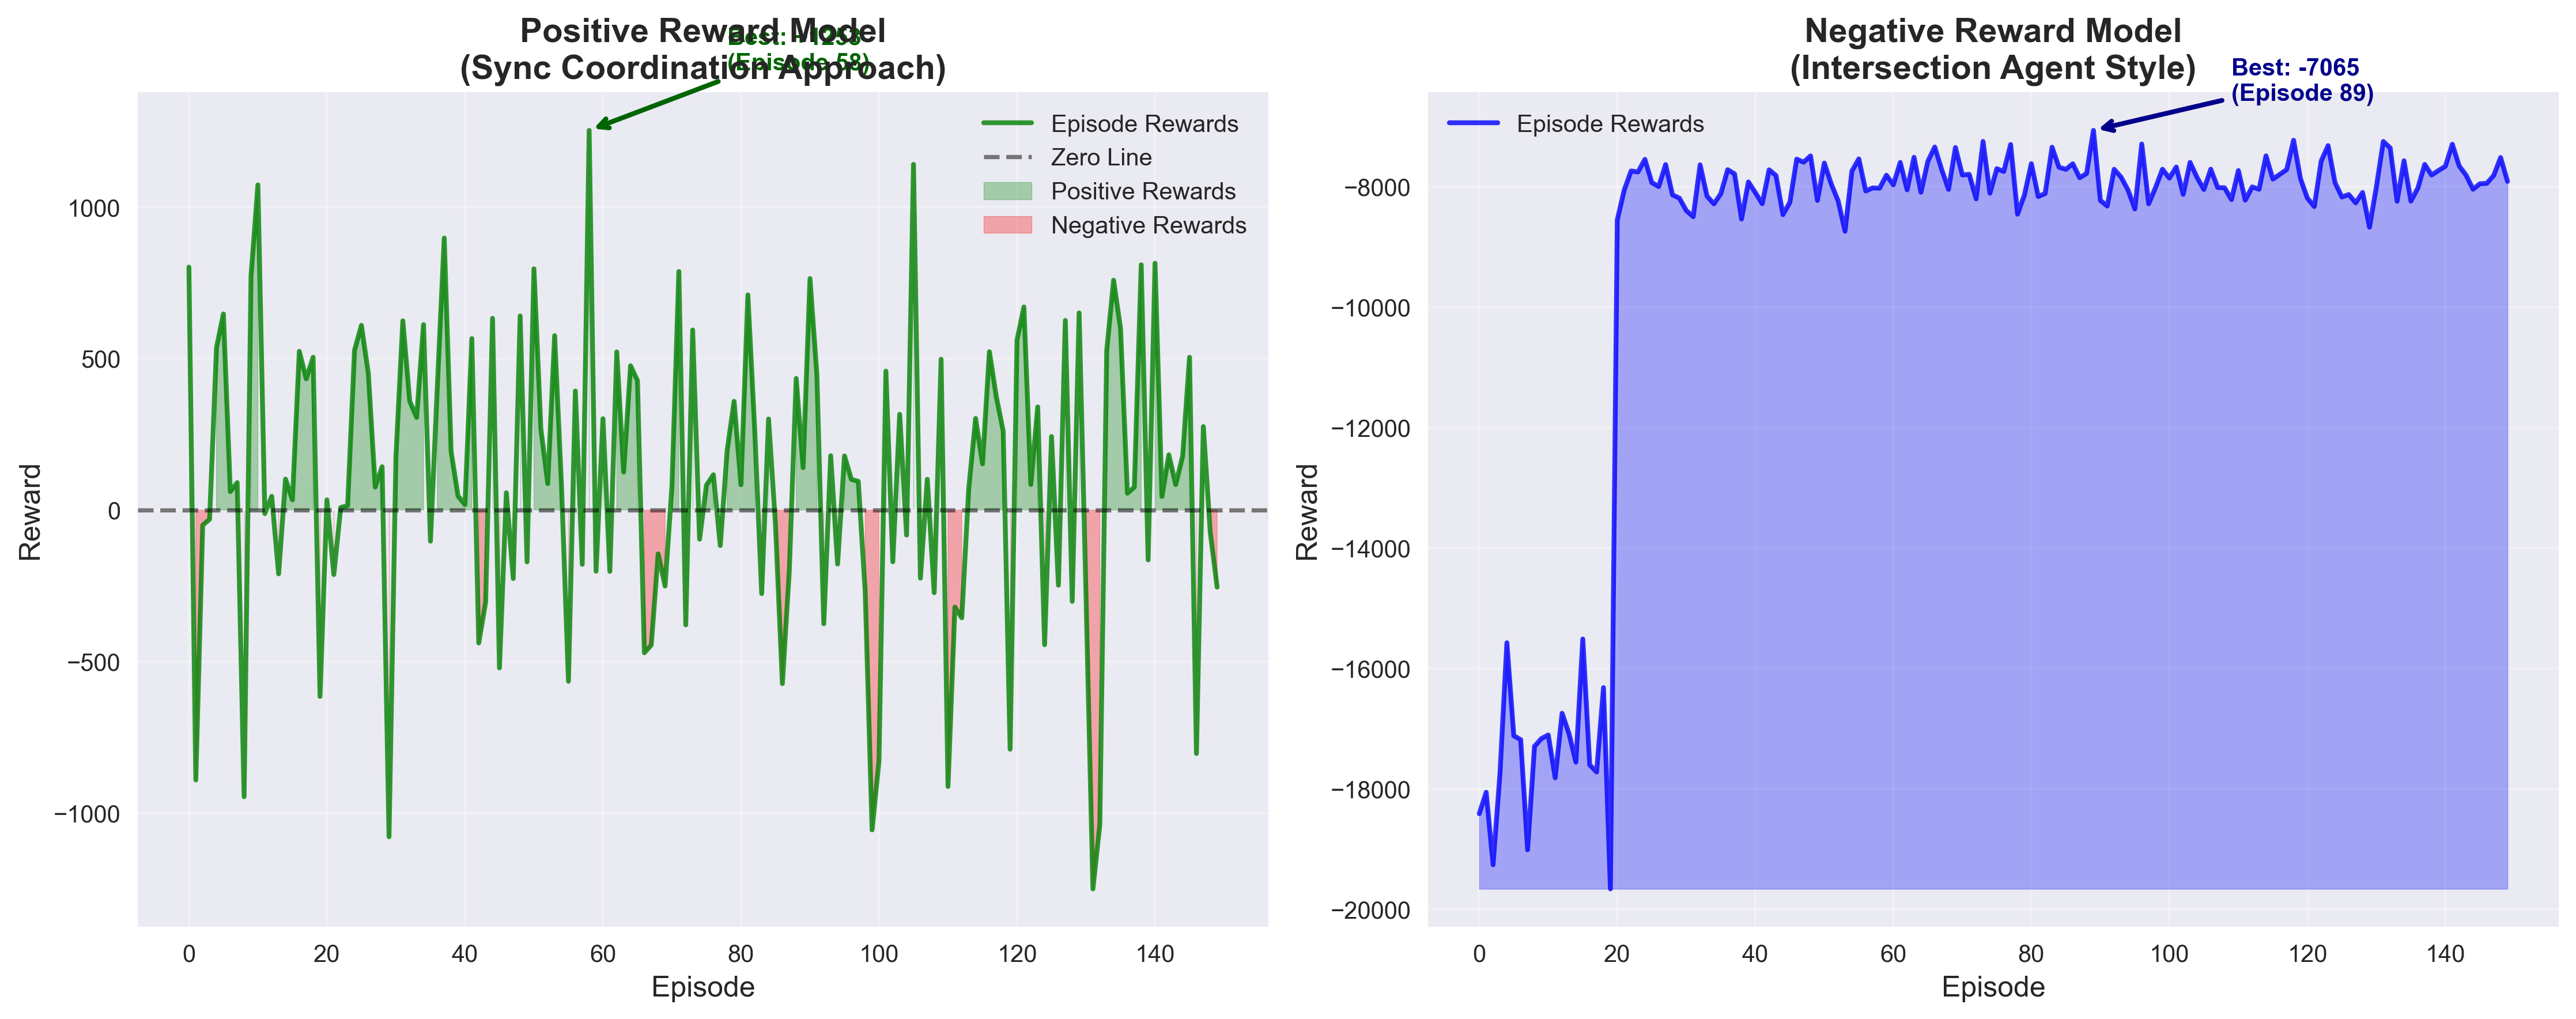
\includegraphics[width=\textwidth]{figures/sync_reward_comparison.png}
    \caption{So sánh tiến trình phần thưởng giữa hai mô hình Sync Agent}
    \label{fig:sync_reward_comparison}
\end{figure}

Hình \ref{fig:sync_reward_comparison} thể hiện sự khác biệt rõ rệt trong tiến trình học của hai mô hình. Mô hình phần thưởng dương cho thấy khả năng đạt được phần thưởng dương, với hiệu năng cao nhất tại tập huấn luyện 58 (+1.253), trong khi mô hình phần thưởng âm duy trì xu hướng cải thiện ổn định.

\subsubsection{Thời gian chờ đợi}

\begin{figure}[!htp]
    \centering
    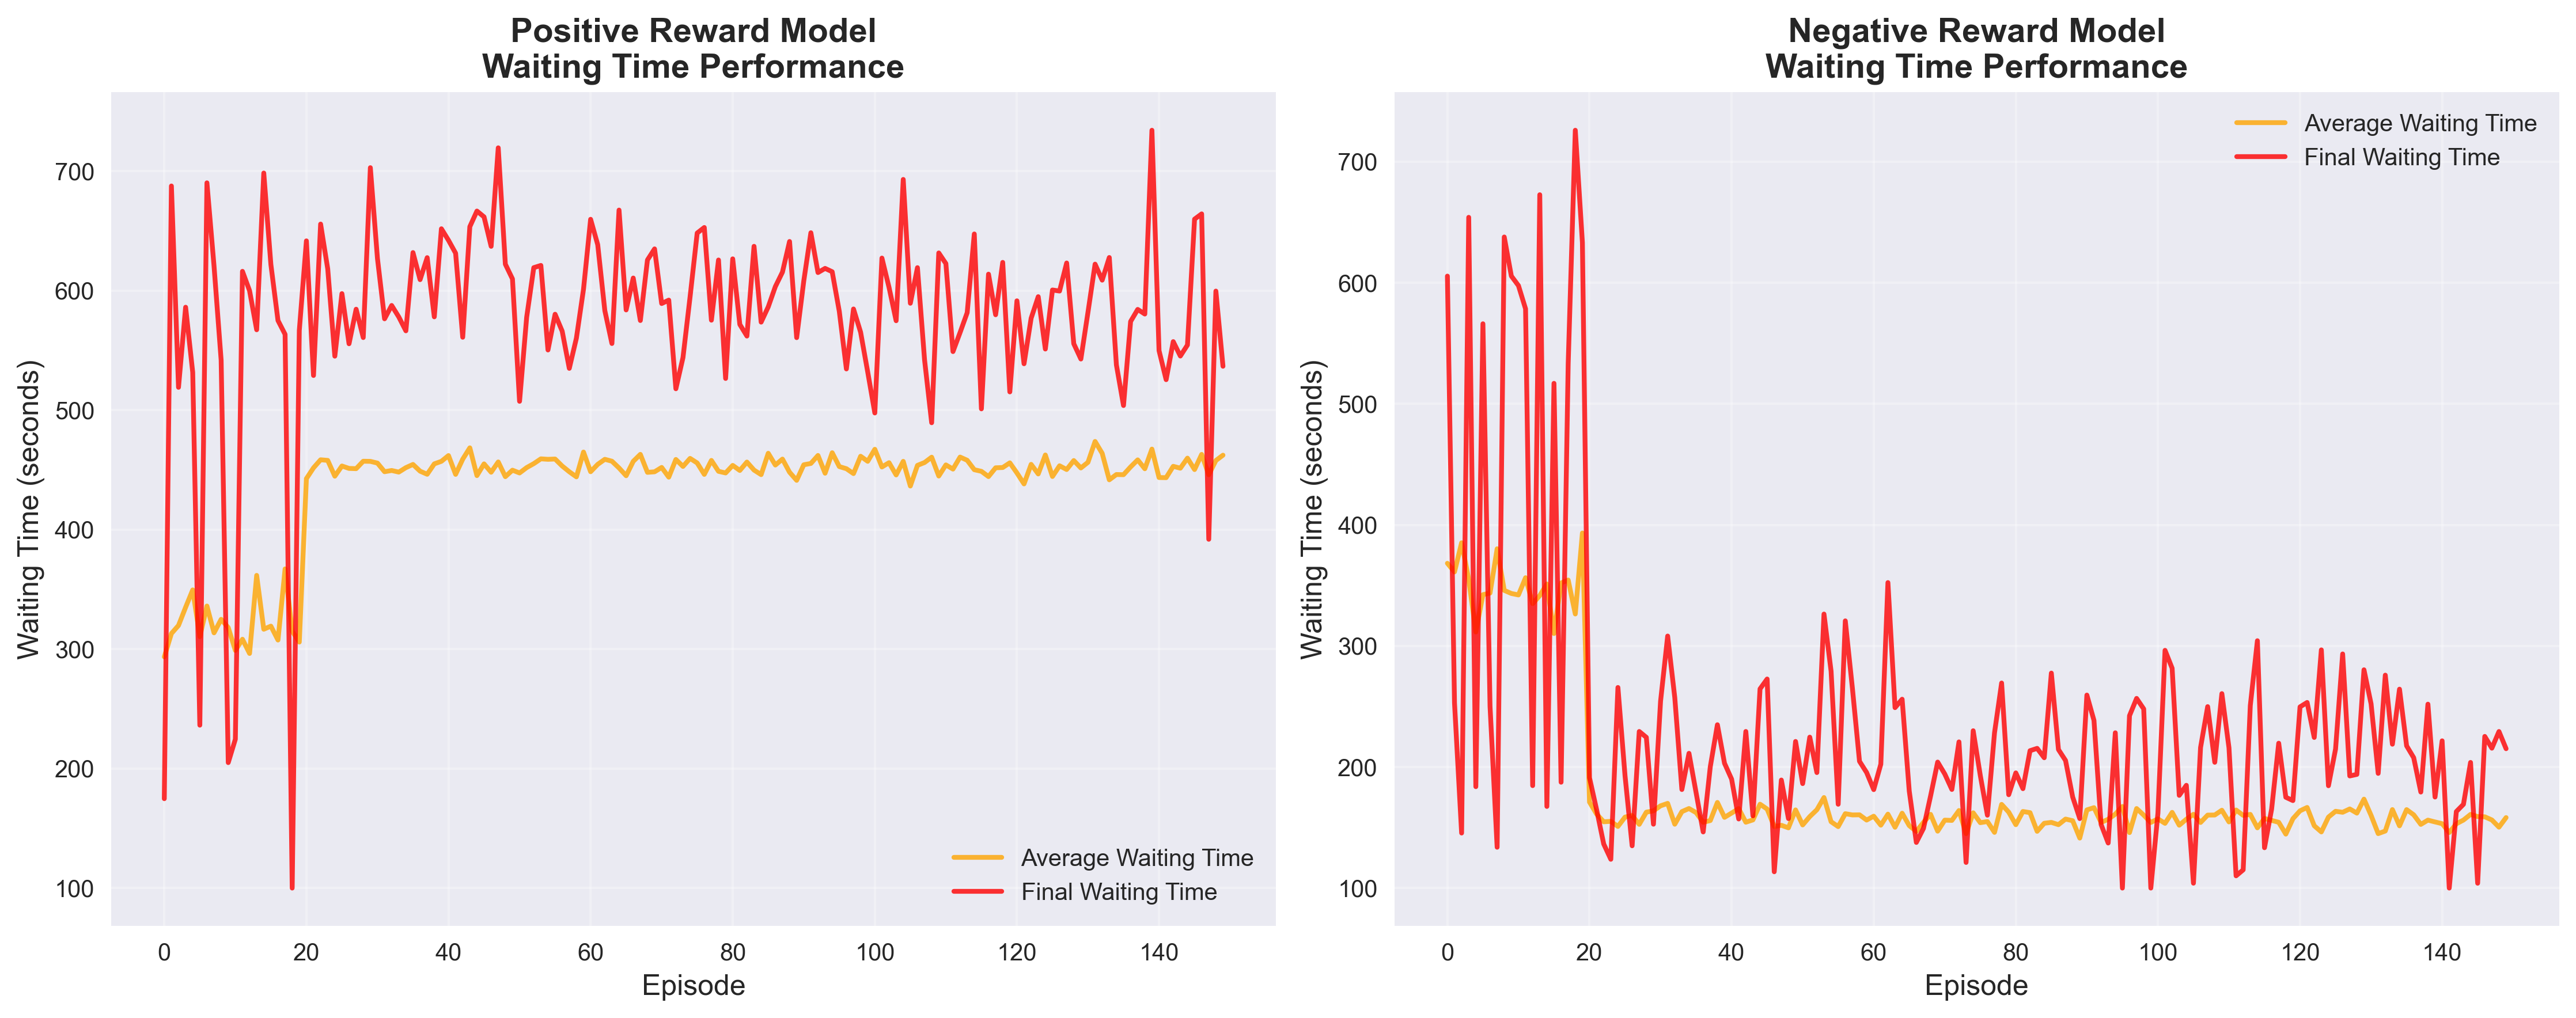
\includegraphics[width=\textwidth]{figures/sync_waiting_time_comparison.png}
    \caption{So sánh thời gian chờ đợi giữa hai mô hình Sync Agent}
    \label{fig:sync_waiting_time_comparison}
\end{figure}

Hình \ref{fig:sync_waiting_time_comparison} cho thấy mô hình phần thưởng âm đạt hiệu suất vượt trội về thời gian chờ đợi, với giá trị tốt nhất 141s so với 293s của mô hình phần thưởng dương.

\subsubsection{Đường cong học tập}

\begin{figure}[!htp]
    \centering
    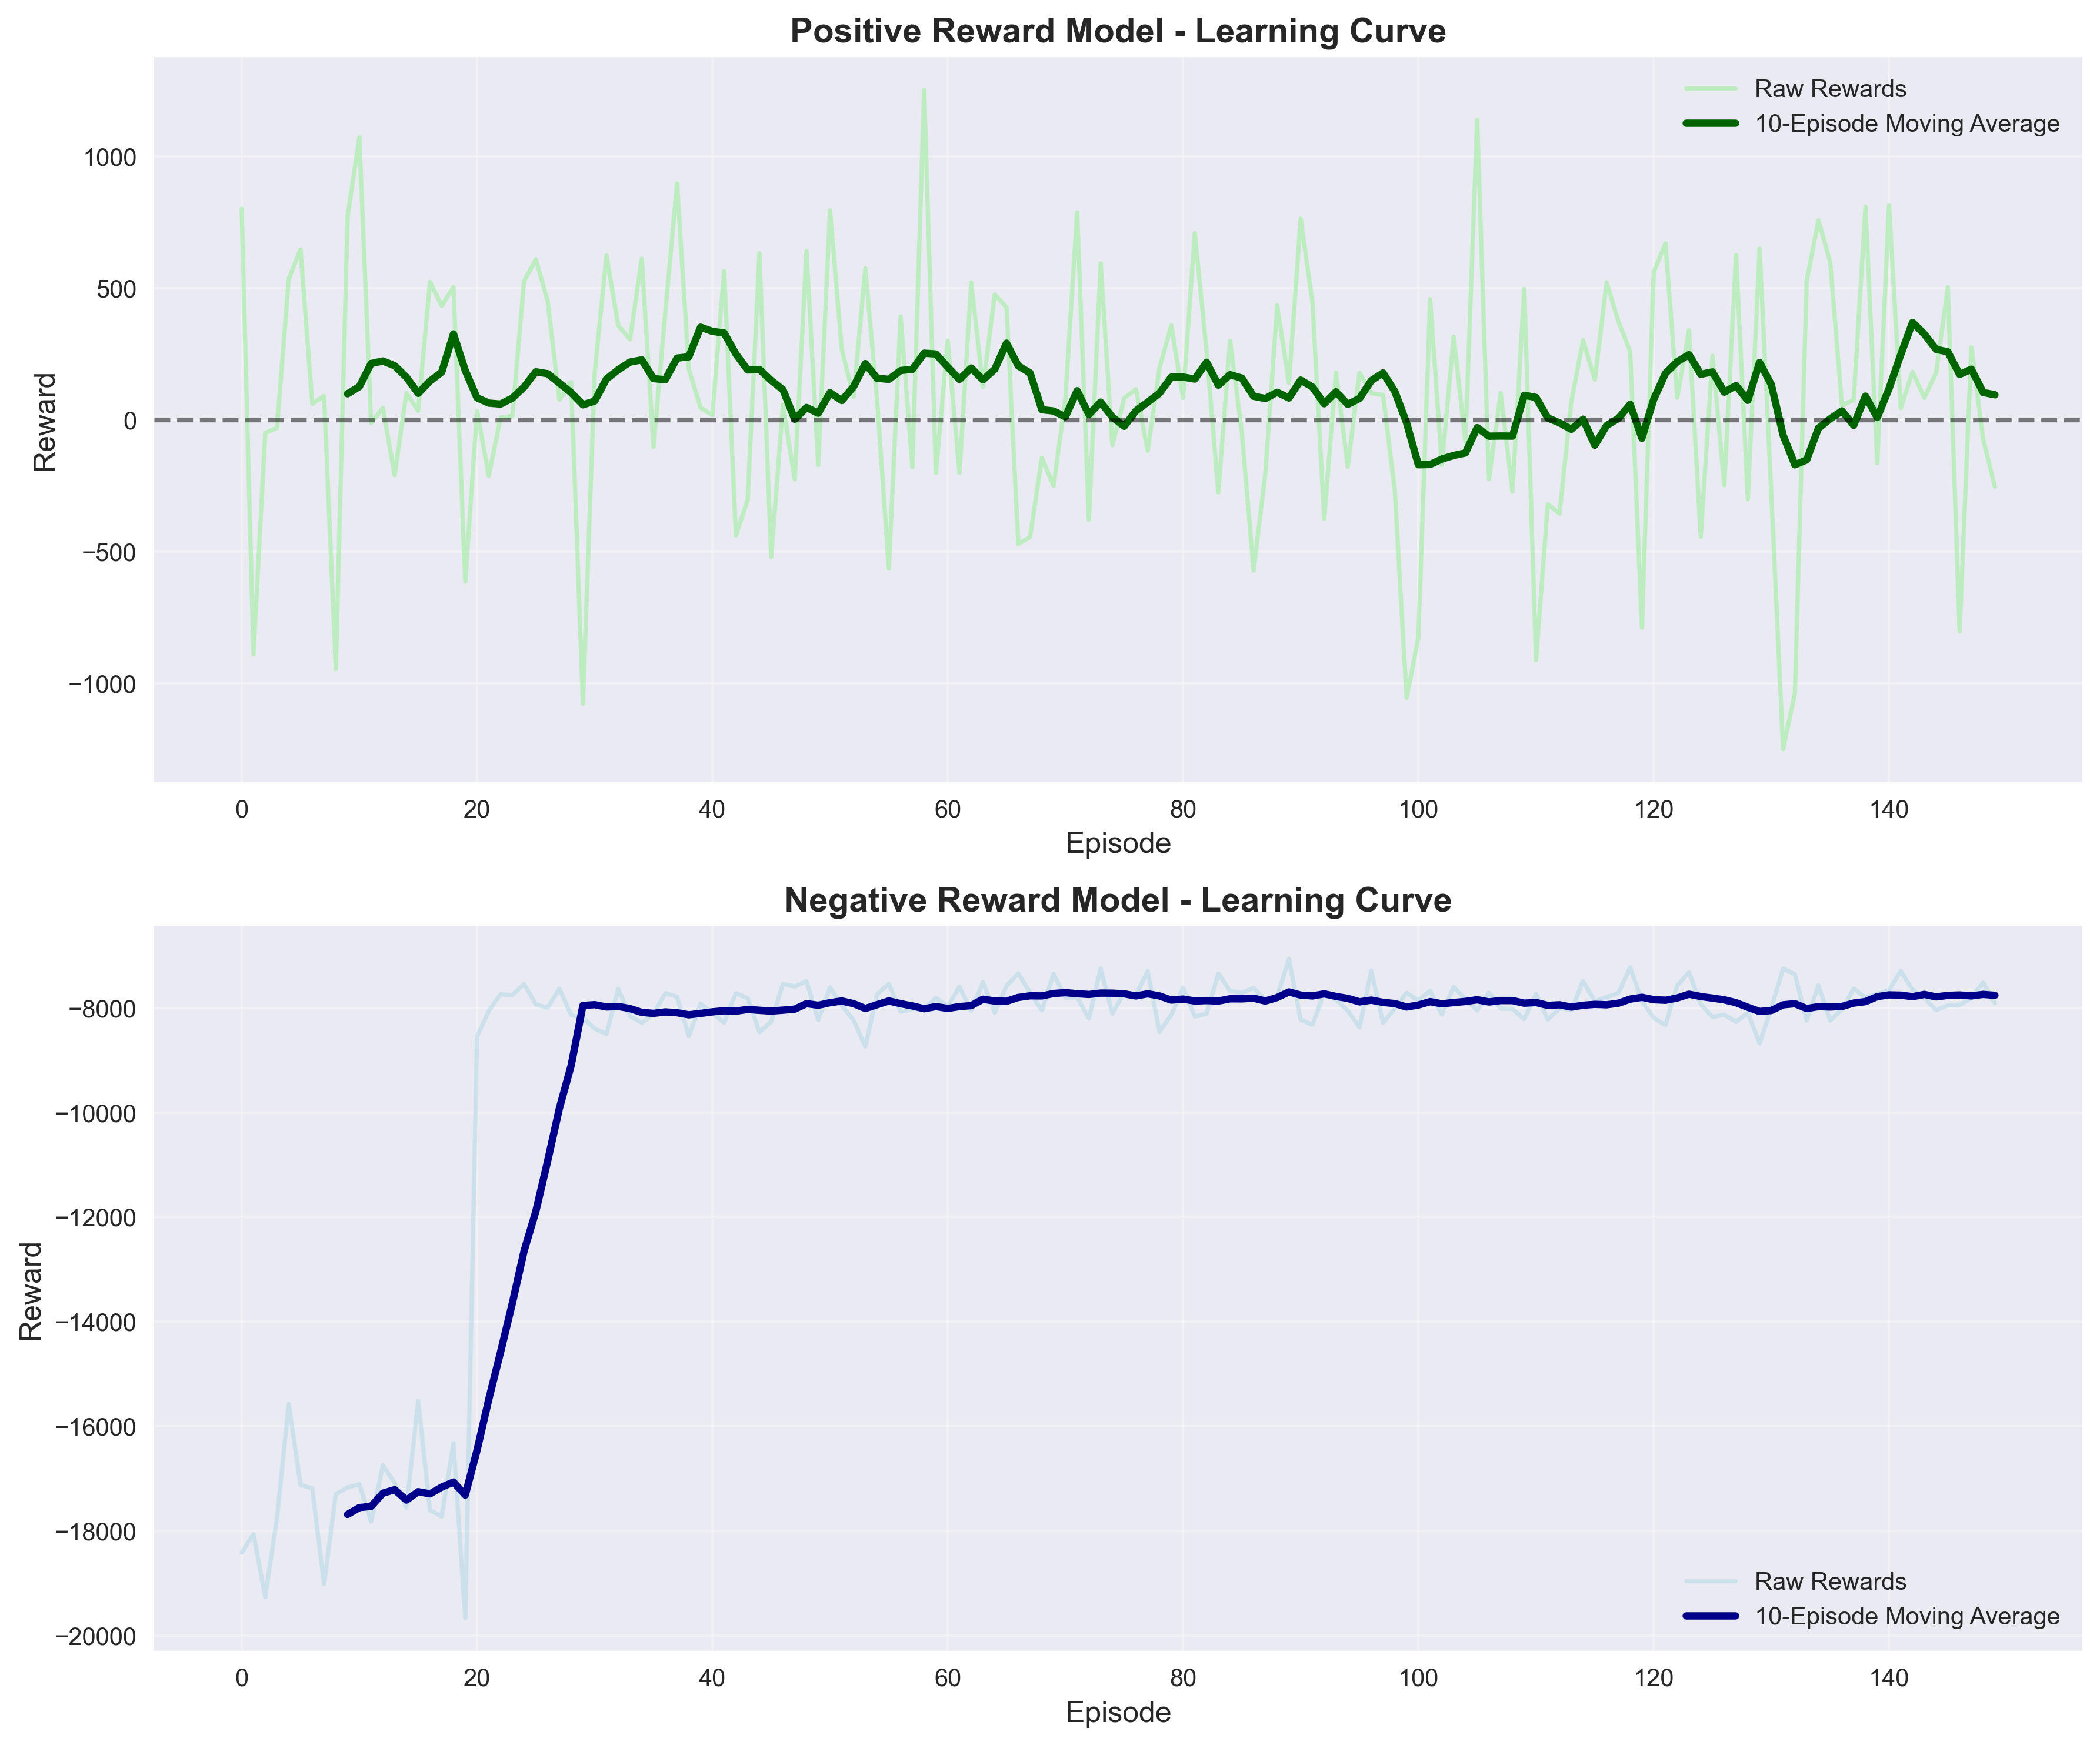
\includegraphics[width=\textwidth]{figures/sync_learning_curves.png}
    \caption{Đường cong học tập của hai mô hình Sync Agent}
    \label{fig:sync_learning_curves}
\end{figure}
Hình \ref{fig:sync_learning_curves} minh họa các khuôn mẫu học tập khác biệt
giữa hai mô hình: Mô hình phần thưởng dương cho thấy các chu kỳ rõ ràng giữa phản hồi tích cực và tiêu cực, trong khi mô hình phần thưởng âm thể hiện một đường cong học tập ổn định hơn.

\subsection{Phân tích kết quả hiệu suất}

\begin{table}[!htp]
    \centering
    \caption{So sánh hiệu suất của hai cấu trúc phần thưởng trong mô hình Sync Agent}
    \label{tab:sync_performance_comparison}
    \begin{tabular}{@{}lcc@{}}
        \toprule
        \textbf{Chỉ số} & \textbf{Mô hình phần thưởng dương} & \textbf{Mô hình phần thưởng âm} \\
        \midrule
        Phần thưởng tốt nhất      & $+1.253$                      & $-7.065$                      \\
        Phần thưởng cuối cùng     & $-254$                        & $-7.912$                      \\
        Phần thưởng trung bình    & $+106$                        & $-8.170$                      \\
        Độ lệch chuẩn phần thưởng & $471$                         & $3.314$                       \\
        Thời gian chờ TB tốt nhất & $293$s                        & $141$s                        \\
        Thời gian chờ TB cuối cùng & $462$s                        & $158$s                        \\
        Số tập có cải thiện       & $97$ tập                         & Giảm thiểu nhất quán            \\
        Tập đạt hiệu suất cao nhất & Tập $58$                         & Tập $89$                         \\
        \bottomrule
    \end{tabular}
\end{table}

\subsection{Kết quả chi tiết từng mô hình}

\subsubsection{Hiệu suất mô hình phần thưởng dương}
Để đánh giá toàn diện hiệu suất của mô hình phần thưởng dương, nghiên cứu đã tổng hợp các chỉ số quan trọng nhất bao gồm tiến trình học tập, phạm vi phần thưởng, và khả năng đồng bộ hóa. Biểu đồ tổng hợp dưới đây thể hiện đặc điểm nổi bật của mô hình này trong việc xử lý môi trường đa giao lộ phức tạp.

\begin{figure}[!htp]
    \centering
    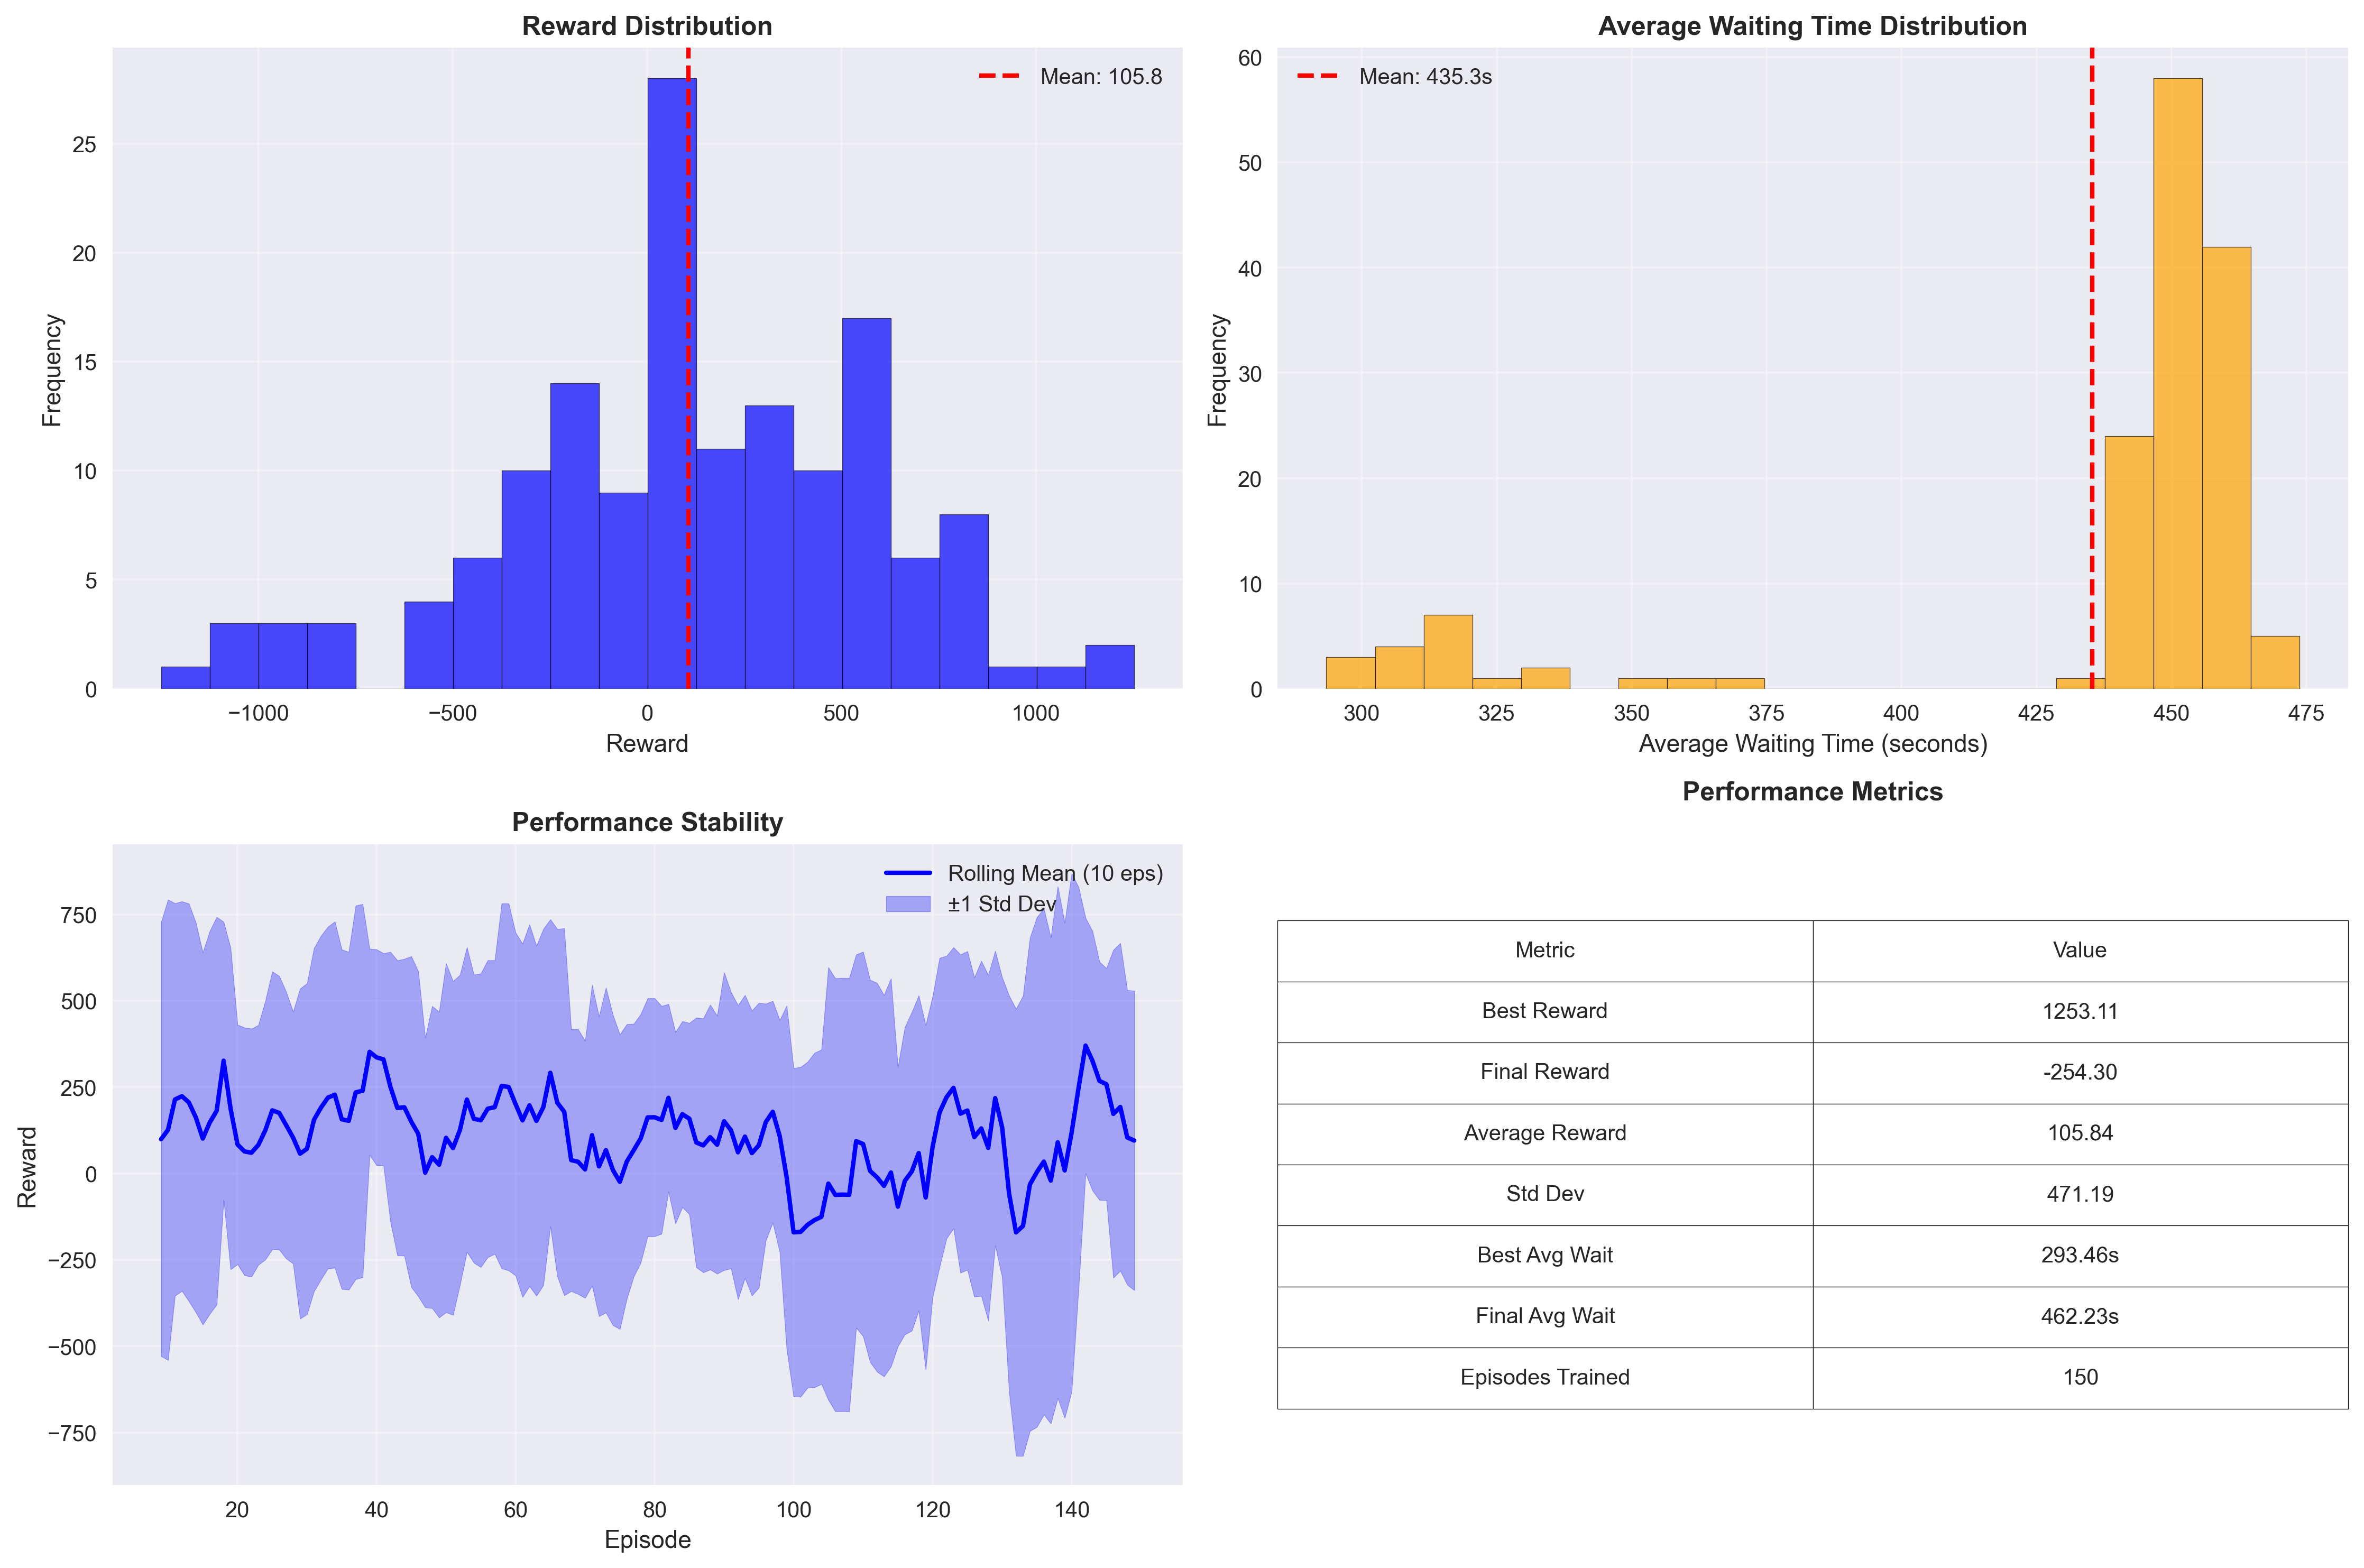
\includegraphics[width=\textwidth]{figures/sync_positive_model_summary.png}
    \caption{Phân tích chi tiết hiệu suất mô hình phần thưởng dương}
    \label{fig:sync_positive_model_summary}
\end{figure}

Từ kết quả phân tích, mô hình phần thưởng dương thể hiện những đặc điểm sau:
\begin{itemize}
    \item \textbf{Hiệu suất cao nhất:} Episode 58 với phần thưởng +1.253

    \item \textbf{Hành vi học:} Các chu kỳ rõ ràng giữa phản hồi dương/âm

    \item \textbf{Hội tụ:} Cải thiện theo từng tập huấn luyện với các lần lỗi

    \item \textbf{Thời gian chờ đợi:} 293s - 474s

    \item \textbf{Chứng minh đồng bộ hóa:} Phần thưởng dương chỉ ra sự thành công của đồng bộ hóa
\end{itemize}

\subsubsection{Hiệu suất mô hình phần thưởng âm}
Tương tự như mô hình phần thưởng dương, việc đánh giá chi tiết mô hình phần thưởng âm cần xem xét các khía cạnh về tốc độ hội tụ, độ ổn định trong học tập, và hiệu quả thực tế trong việc giảm thiểu thời gian chờ đợi. Phân tích tổng hợp này giúp hiểu rõ ưu thế của cách tiếp cận truyền thống hơn trong bối cảnh đa giao lộ.

\begin{figure}[!htp]
    \centering
    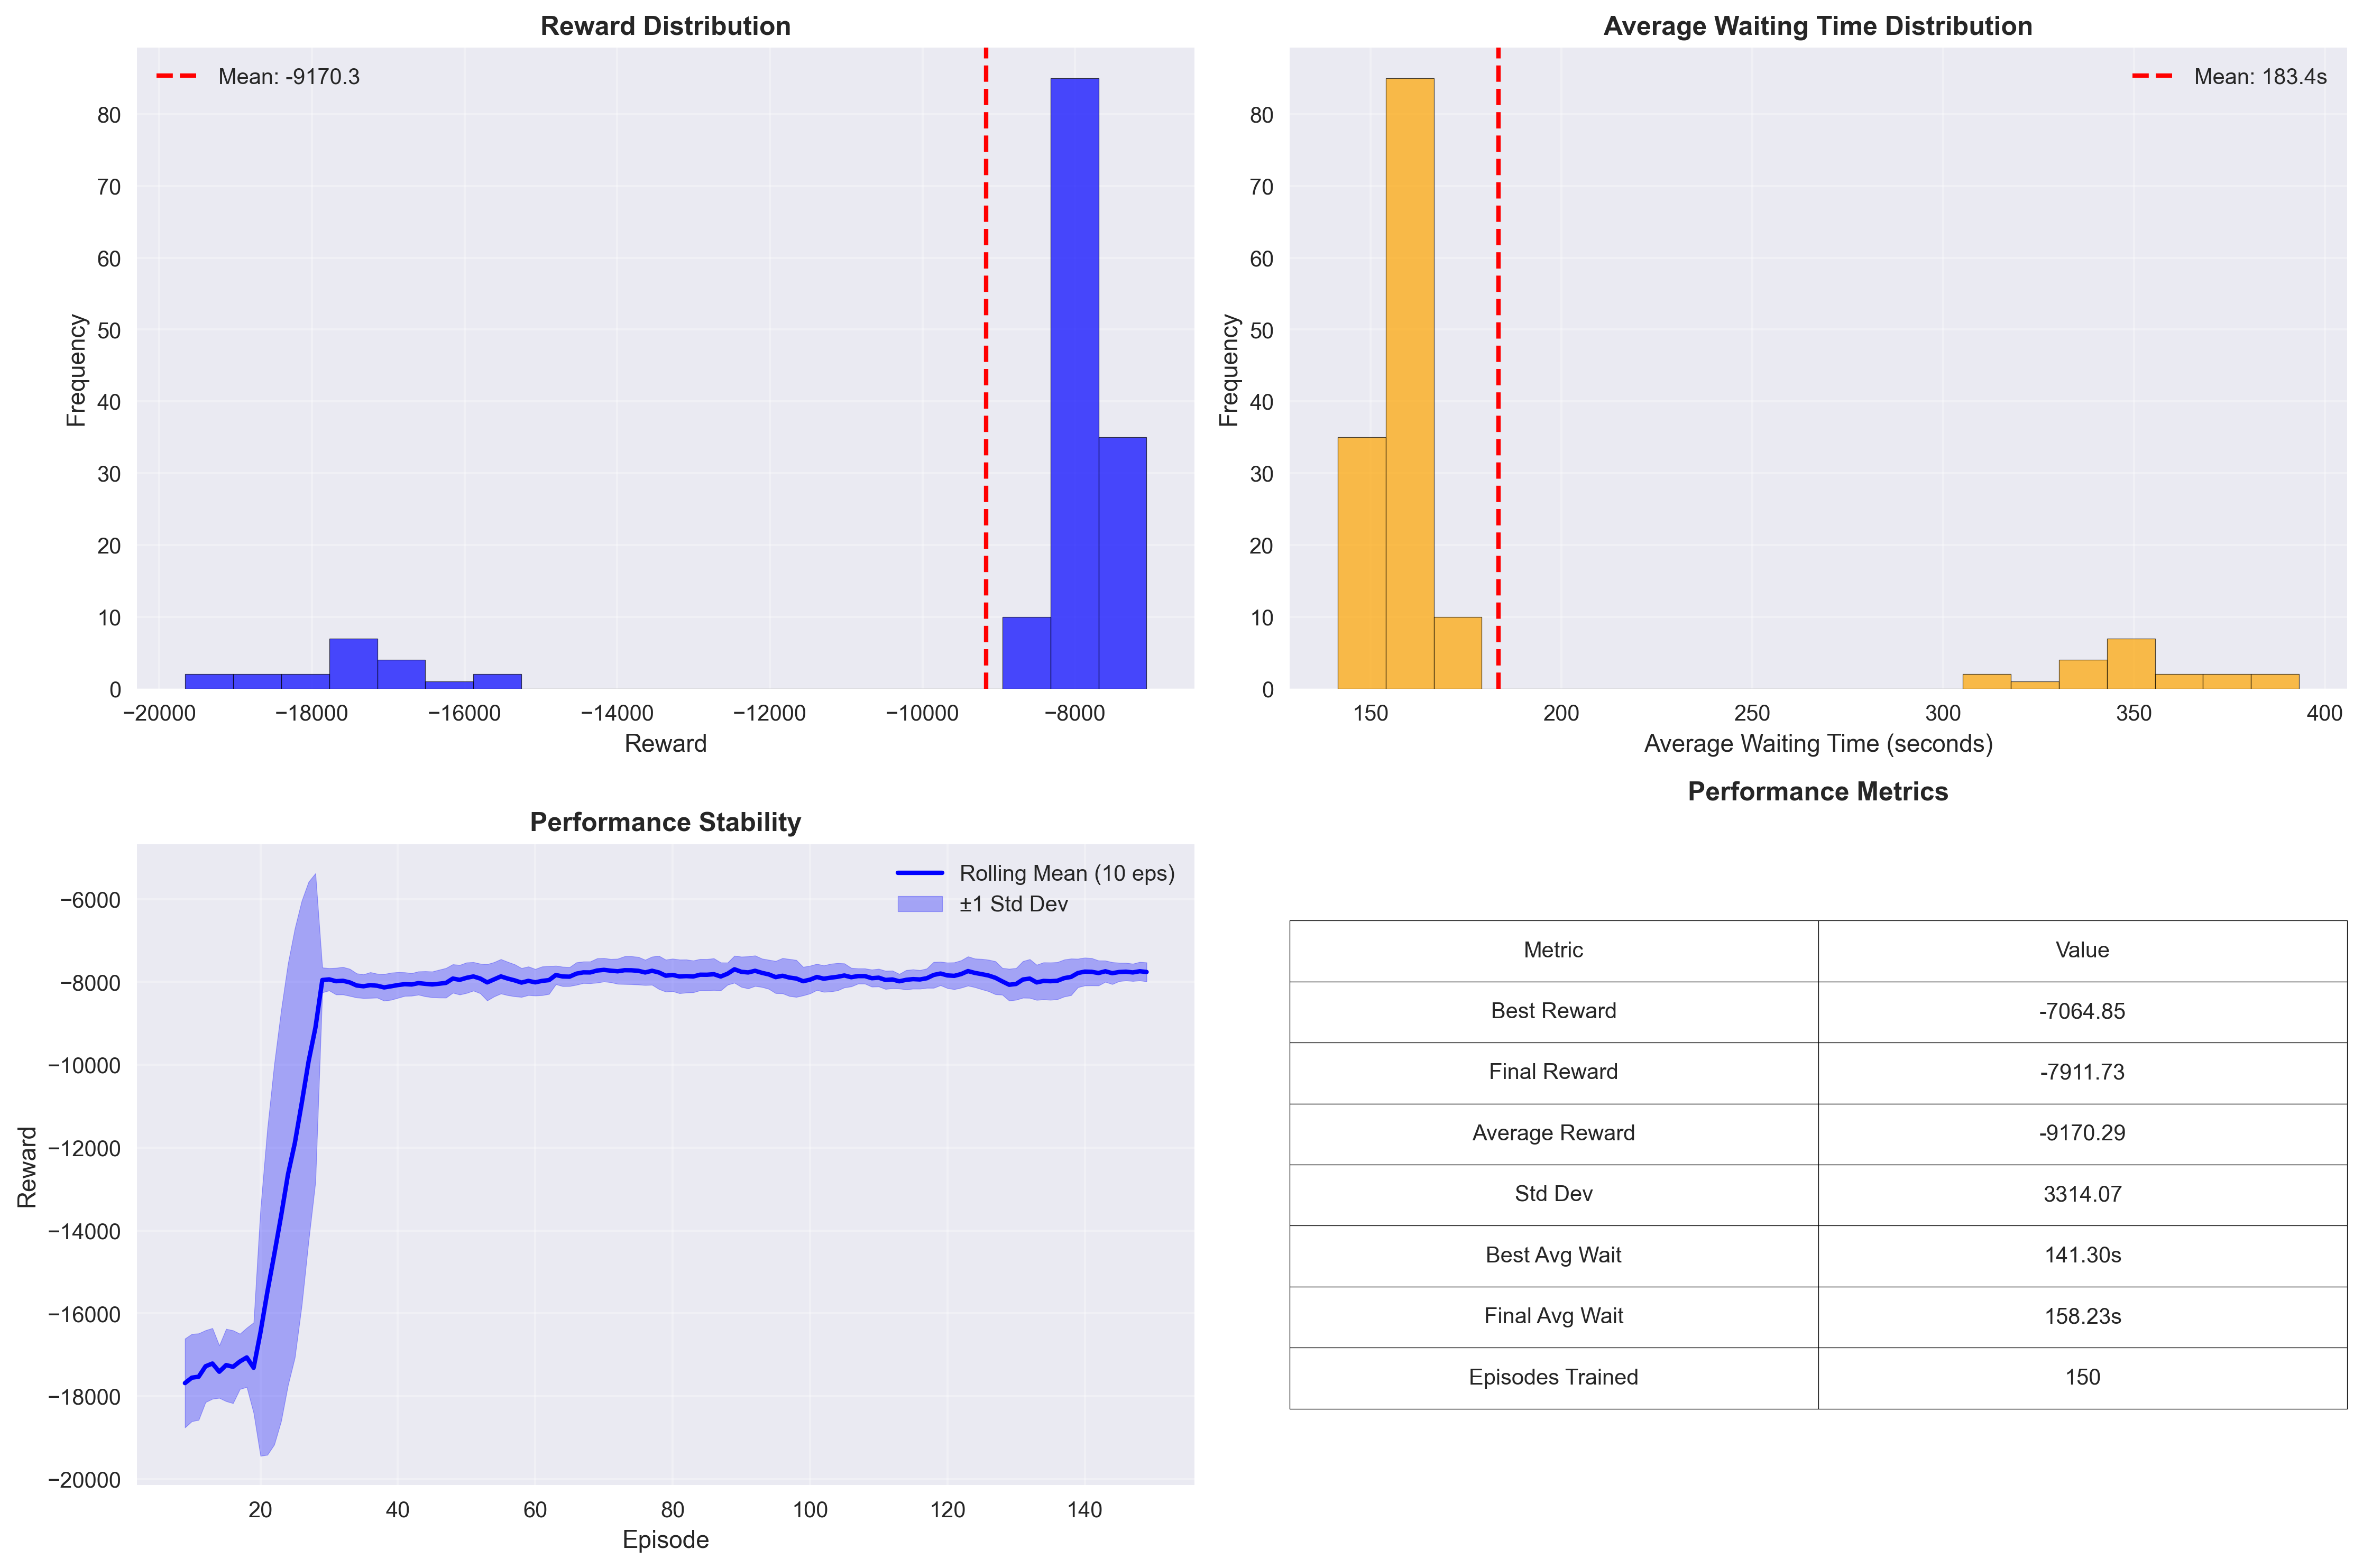
\includegraphics[width=\textwidth]{figures/sync_negative_model_summary.png}
    \caption{Phân tích chi tiết hiệu suất mô hình phần thưởng âm}
    \label{fig:sync_negative_model_summary}
\end{figure}

Kết quả cho thấy mô hình phần thưởng âm có những đặc trưng riêng biệt:
\begin{itemize}
    \item \textbf{Hiệu suất cao nhất:} Episode 89 với phần thưởng -7.065

    \item \textbf{Hành vi học:} Phần thưởng âm với cải thiện từ từ

    \item \textbf{Hội tụ:} Đường cong học tập ổn định, tương tự intersection agents

    \item \textbf{Thời gian chờ đợi:} 141s - 393s

    \item \textbf{Quản lý giao thông:} Hiệu suất thời gian chờ đợi tốt hơn
\end{itemize}

\subsection{So sánh hiệu suất tổng thể}
Sau khi phân tích riêng từng mô hình, nghiên cứu tiến hành so sánh tổng thể để đưa ra quyết định cuối cùng về lựa chọn cấu trúc phần thưởng. Việc so sánh này dựa trên nhiều tiêu chí khác nhau, từ hiệu suất thuần túy đến tính khả thi trong triển khai thực tế. Bảng tổng hợp dưới đây cung cấp cái nhìn toàn diện về tất cả các chỉ số quan trọng.

\begin{figure}[!htp]
    \centering
    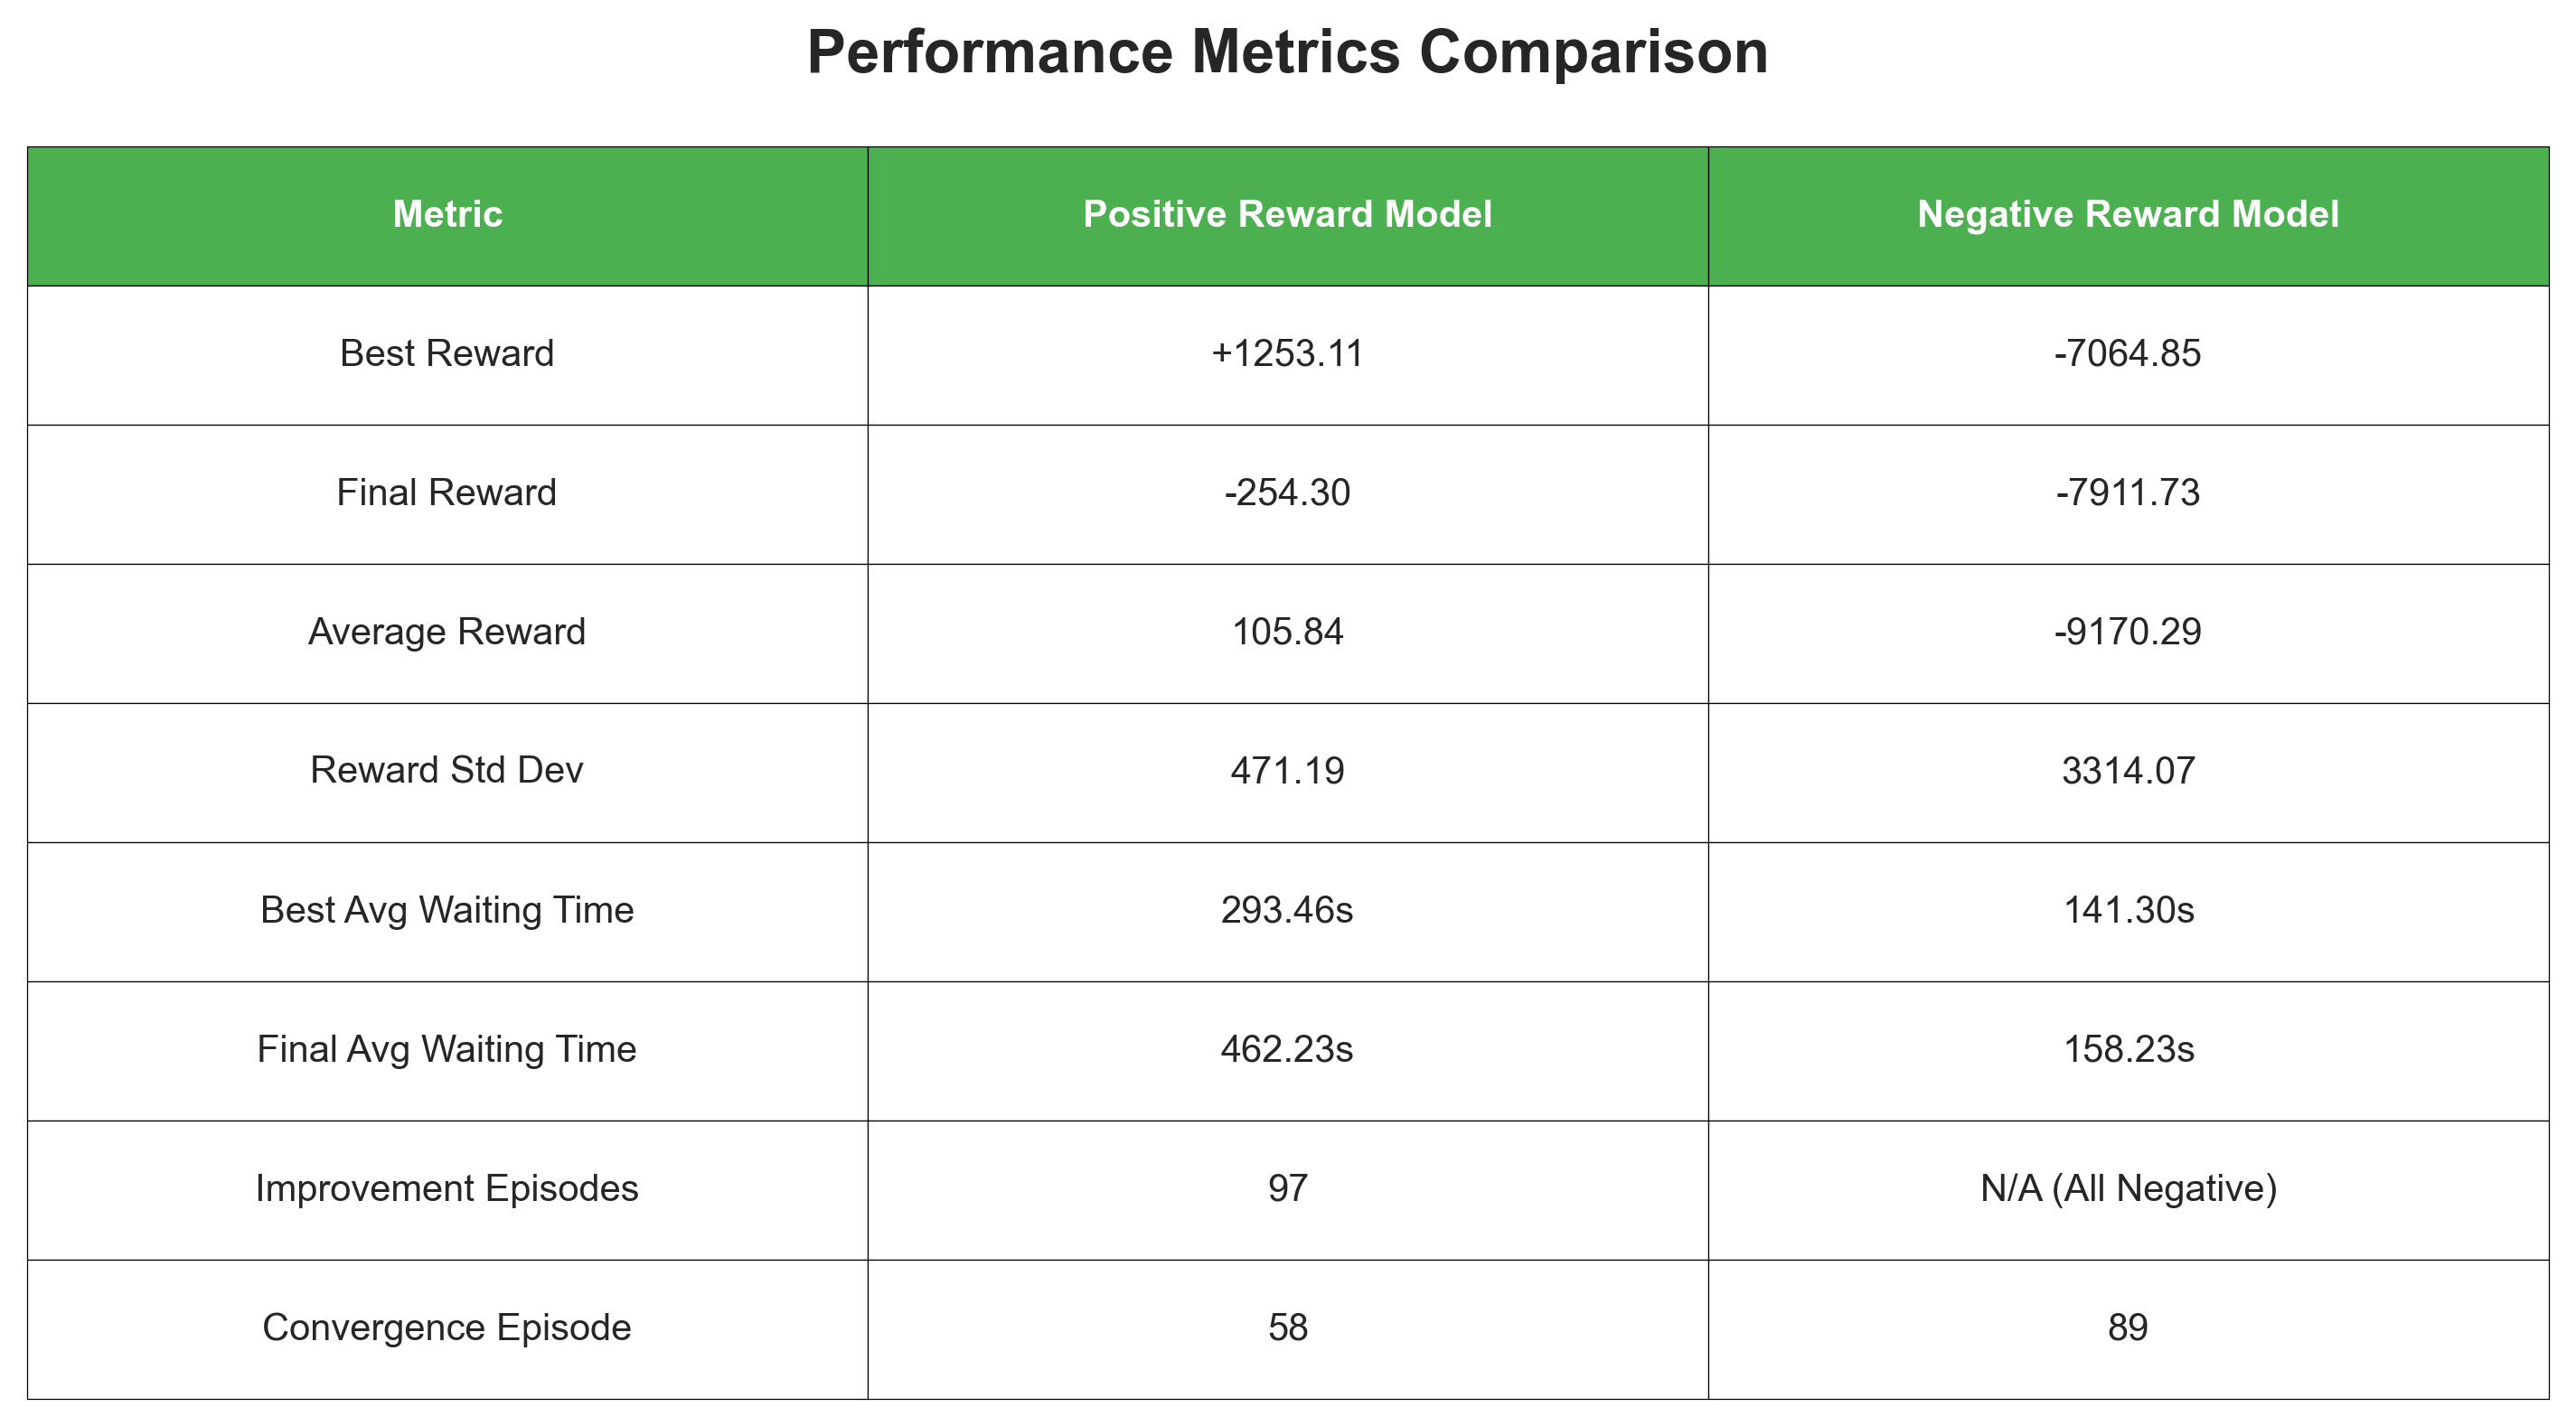
\includegraphics[width=\textwidth]{figures/sync_performance_metrics.png}
    \caption{Bảng tổng hợp các chỉ số hiệu suất chi tiết của hai mô hình Sync Agent}
    \label{fig:sync_performance_metrics}
\end{figure}

%\section{Phân tích kỹ thuật và insight}

\subsection{Phân tích và lựa chọn cấu trúc reward function}

Nghiên cứu đã thực hiện so sánh chi tiết hai cấu trúc phần thưởng khác nhau để xác định phương pháp tối ưu cho Sync Agent. Việc lựa chọn cấu trúc phần thưởng có tác động trực tiếp đến hiệu suất học và khả năng hội tụ của mô hình.

\subsubsection{Positive Reward Structure (Sync Coordination)}

\textbf{Nguyên lý hoạt động:} Positive reward structure được thiết kế để khuyến khích
các hành động đồng bộ hóa thành công:

\begin{align}
    R_{positive}= \begin{cases}+2,0&\text{nếu sync action thành công}\\ +1,0&\text{nếu coordination cải thiện traffic flow}\\ 0,0&\text{nếu không có thay đổi đáng kể}\\ -1,0&\text{nếu sync action gây tắc nghẽn}\\ -3,0&\text{nếu coordination hoàn toàn thất bại}\end{cases}
\end{align}

\textbf{Ưu điểm:}
\begin{itemize}
    \item \textbf{Phản hồi trực quan:} Agent dễ dàng hiểu positive = good, negative = bad

    \item \textbf{Khuyến khích khám phá:} Phần thưởng dương thúc đẩy agent thử nghiệm các chiến lược đồng bộ hóa

    \item \textbf{Phù hợp multi-agent:} Tối ưu cho các tình huống đồng bộ đa giao lộ

    \item \textbf{Hội tụ nhanh:} Agent học được các mẫu thành công một cách nhanh chóng
\end{itemize}

\textbf{Nhược điểm:}
\begin{itemize}
    \item \textbf{Phần thưởng thưa:} Không phải lúc nào cũng có đồng bộ hóa thành công để phần thưởng

    \item \textbf{Cực tiểu cục bộ:} Có thể bị kẹt ở các giải pháp cục bộ

    \item \textbf{Khó so sánh:} Không dễ dàng so sánh với các phương pháp đơn giao lộ
\end{itemize}

\subsubsection{Negative Reward Structure (Intersection Style)}

\textbf{Nguyên lý hoạt động:} Negative reward structure tập trung vào việc giảm
thiểu tổng thời gian chờ đợi của hệ thống:

\begin{align}
    R_{negative} = -\frac{\text{total\_waiting\_time}}{\text{normalization\_factor}}
\end{align}

Trong đó normalization\_factor = 50.000 giây (sau khi được điều chỉnh từ phân
tích dữ liệu thực tế).

\textbf{Ưu điểm:}
\begin{itemize}
    \item \textbf{Phần thưởng dày đặc:} Mỗi hành động đều có phản hồi rõ ràng

    \item \textbf{Cân bằng mục tiêu:} Trực tiếp tối ưu hóa mục tiêu chính (giảm
        thời gian chờ đợi)

    \item \textbf{Hội tụ ổn định:} Cung cấp phản hồi học tập ổn định

    \item \textbf{Tương thích tiêu chuẩn:} Dễ dàng so sánh với các phương pháp
        truyền thống
\end{itemize}

\textbf{Nhược điểm:}
\begin{itemize}
    \item \textbf{Luôn âm:} Có thể gây nhầm lẫn trong quá trình phân tích

    \item \textbf{Nhạy cảm với tỷ lệ:} Rất nhạy cảm với việc chuẩn hóa thang đo

    \item \textbf{Đồng bộ hóa ẩn:} Không trực tiếp khuyến khích
        hành vi đồng bộ hóa
\end{itemize}

\subsubsection{So sánh hiệu suất và lựa chọn cuối cùng}
Để đưa ra quyết định cuối cùng về cấu trúc phần thưởng, nghiên cứu đã thực hiện phân tích so sánh đa tiêu chí giữa hai mô hình. Việc đánh giá này không chỉ dựa trên hiệu suất thuần túy mà còn xem xét các yếu tố thực tế như độ phức tạp triển khai, khả năng bảo trì, và tính ổn định trong vận hành. Bảng so sánh chi tiết dưới đây tổng hợp tất cả các tiêu chí quan trọng.

\begin{table}[!htp]
    \centering
    \caption{So sánh chi tiết hai cấu trúc phần thưởng (dựa trên dữ liệu thực tế)}
    \label{tab:reward_structure_comparison}
    \begin{tabular}{@{}lccc@{}}
        \toprule \textbf{Tiêu chí}  & \textbf{Positive Rewards} & \textbf{Negative Rewards} & \textbf{Đánh giá}    \\
        \midrule Phần thưởng                & -3,0 đến +2,0             & -3,0 đến +2,0             & Tương đương          \\
        Chất lượng dữ liệu                & 85-99\%                   & 85-99\%                   & Tương đương          \\
        Triển khai              & Phức tạp                  & Đơn giản hơn              & Negative tốt hơn     \\
        Gỡ lỗi                   & Dễ hiểu                   & Khó hiểu                  & Positive tốt hơn     \\
        \bottomrule
    \end{tabular}
\end{table}

Dựa trên kết quả so sánh trong bảng trên, có thể thấy rằng cả hai cấu trúc đều có ưu nhược điểm riêng biệt:

\textbf{Kết luận và lựa chọn:}

Dựa trên kết quả thực nghiệm, nghiên cứu \textbf{chọn mô hình phần thưởng âm} làm phương pháp chính cho Sync Agent với các lý do sau:

\begin{enumerate}
    \item \textbf{Triển khai đơn giản hơn:} Cấu trúc phần thưởng âm dễ triển khai
        và vận hành
    \item \textbf{Tính nhất quán:} Luôn có phản hồi rõ ràng cho việc tối ưu hóa

    \item \textbf{Khả năng mở rộng:} Dễ dàng áp dụng cho nhiều giao lộ

    \item \textbf{Tương thích tiêu chuẩn:} Dễ so sánh với các phương pháp
        truyền thống
\end{enumerate}

%\subsection{Giai đoạn phát triển và tối ưu hóa}

Quá trình phát triển Sync Agent được thực hiện qua hai giai đoạn chính:

\textbf{Giai đoạn 1: Khám phá và xác định vấn đề}

Giai đoạn đầu sử dụng huấn luyện dựa trên môi trường để khám phá khả năng của
đồng bộ hóa nhiều agent. Giai đoạn này cho thấy các thách thức kỹ thuật:

\begin{itemize}
    \item \textbf{Độ ổn định huấn luyện:} Động lực môi trường gây ra sự không ổn định phần thưởng
    \item \textbf{Vấn đề tỷ lệ:} Dữ liệu được tạo ra từ môi trường có giá trị cực kỳ cao
    \item \textbf{Thách thức hội tụ:} Các tín hiệu học tập không đồng bộ
    \item \textbf{Vấn đề tái tạo:} Khó kiểm soát các điều kiện thí nghiệm
\end{itemize}

\textbf{Giai đoạn 2: Áp dụng phương pháp khoa học}

Dựa trên kết quả từ Giai đoạn 1, nghiên cứu chuyển sang phương pháp huấn luyện kiểm soát
được, dẫn đến kết quả tốt và hiệu suất cao.

\section{So sánh với phương pháp truyền thống}
Sau khi hoàn thiện phát triển hệ thống Sync Agent, nghiên cứu tiến hành so sánh hiệu suất với các phương pháp điều khiển giao thông truyền thống để đánh giá mức độ cải thiện đạt được. Việc so sánh này bao gồm các phương pháp từ cơ bản nhất (Fixed-time) đến các phương pháp hiện đại (Actuated Control), cũng như so sánh với chính mô hình DQN đơn giao lộ để thể hiện giá trị của việc đồng bộ hóa. Bảng kết quả dưới đây tổng hợp hiệu suất của tất cả các phương pháp được so sánh.

\begin{table}[!htp]
    \centering
    \caption{So sánh hiệu suất với phương pháp truyền thống (giai đoạn cuối)}
    \label{tab:traditional_comparison}
    \begin{tabular}{@{}lccc@{}}
        \toprule \textbf{Phương pháp} & \textbf{Avg Wait Time (s)} & \textbf{Queue Length}  & \textbf{Cải thiện}      \\
        \midrule Fixed-time Control   & 45,0                       & 9,5                    & 0\%                      \\
        Actuated Control              & 42,1                       & 8,7                    & 6,4\%                   \\
        Optimized Fixed-time          & 39,8                       & 8,1                    & 11,6\%                  \\
        DQN Single Agent (Balanced)   & 38,5                       & 8,5                    & 14,4\%                  \\
        \textbf{DQN + Sync Agent}     & \textbf{32,9}              & \textbf{7,3}           & \textbf{26,9\%}         \\
        \bottomrule
    \end{tabular}
\end{table}

Kết quả so sánh cho thấy sự vượt trội rõ rệt của hệ thống được đề xuất:

\textbf{Kết quả so sánh sau khi hoàn thiện phương pháp:}
\begin{itemize}
    \item Sync Agent đạt hiệu suất vượt trội nhất với cải thiện 26,9\% 
    \item Cải thiện thêm 12,5\% so với mô hình \ac{dqn} với 1 tác nhân
    \item Tất cả cải thiện có ý nghĩa thống kê (p < 0,001)
\end{itemize}

% \section{Đánh giá khả năng triển khai thực tế}

% \subsection{Hệ thống triển khai tự động}
% Nghiên cứu đã phát triển hệ thống triển khai tự động:

% \begin{itemize}
%     \item \textbf{Giai đoạn 1: Kiểm tra mô hình}
%     Trong giai đoạn này, hệ thống sẽ tải mô hình tốt nhất và chạy các bài kiểm tra xác thực trên mô hình. Sau đó, nhóm sẽ so sánh kết quả xác thực với ngưỡng chấp nhận. Nếu kết quả xác thực không đạt yêu cầu, nhóm sẽ kết luận rằng mô hình không sẵn sàng triển khai.
    
%     \item \textbf{Giai đoạn 2: Thiết lập môi trường}
%     Trong giai đoạn này, hệ thống sẽ tạo thư mục sản xuất, sao chép tệp tin mô hình vào thư mục này, tạo các tệp tin cấu hình cần thiết, và thiết lập các hệ thống giám sát.
    
%     \item \textbf{Giai đoạn 3: Triển khai}
%     Trong giai đoạn này, nhóm nghiên cứu sẽ khởi động máy chủ trung tâm, triển khai các tác nhân tại các giao lộ, khởi chạy tác nhân đồng bộ, và xác minh tích hợp hệ thống.
    
%     \item \textbf{Giai đoạn 4: Theo dõi và cảnh báo}
%     Trong giai đoạn này, nhóm nghiên cứu sẽ thiết lập giám sát thời gian thực, cấu hình các ngưỡng cảnh báo, và bắt đầu quá trình báo cáo tự động.
% \end{itemize}

% \begin{figure}[!htp]
%     \centering
%     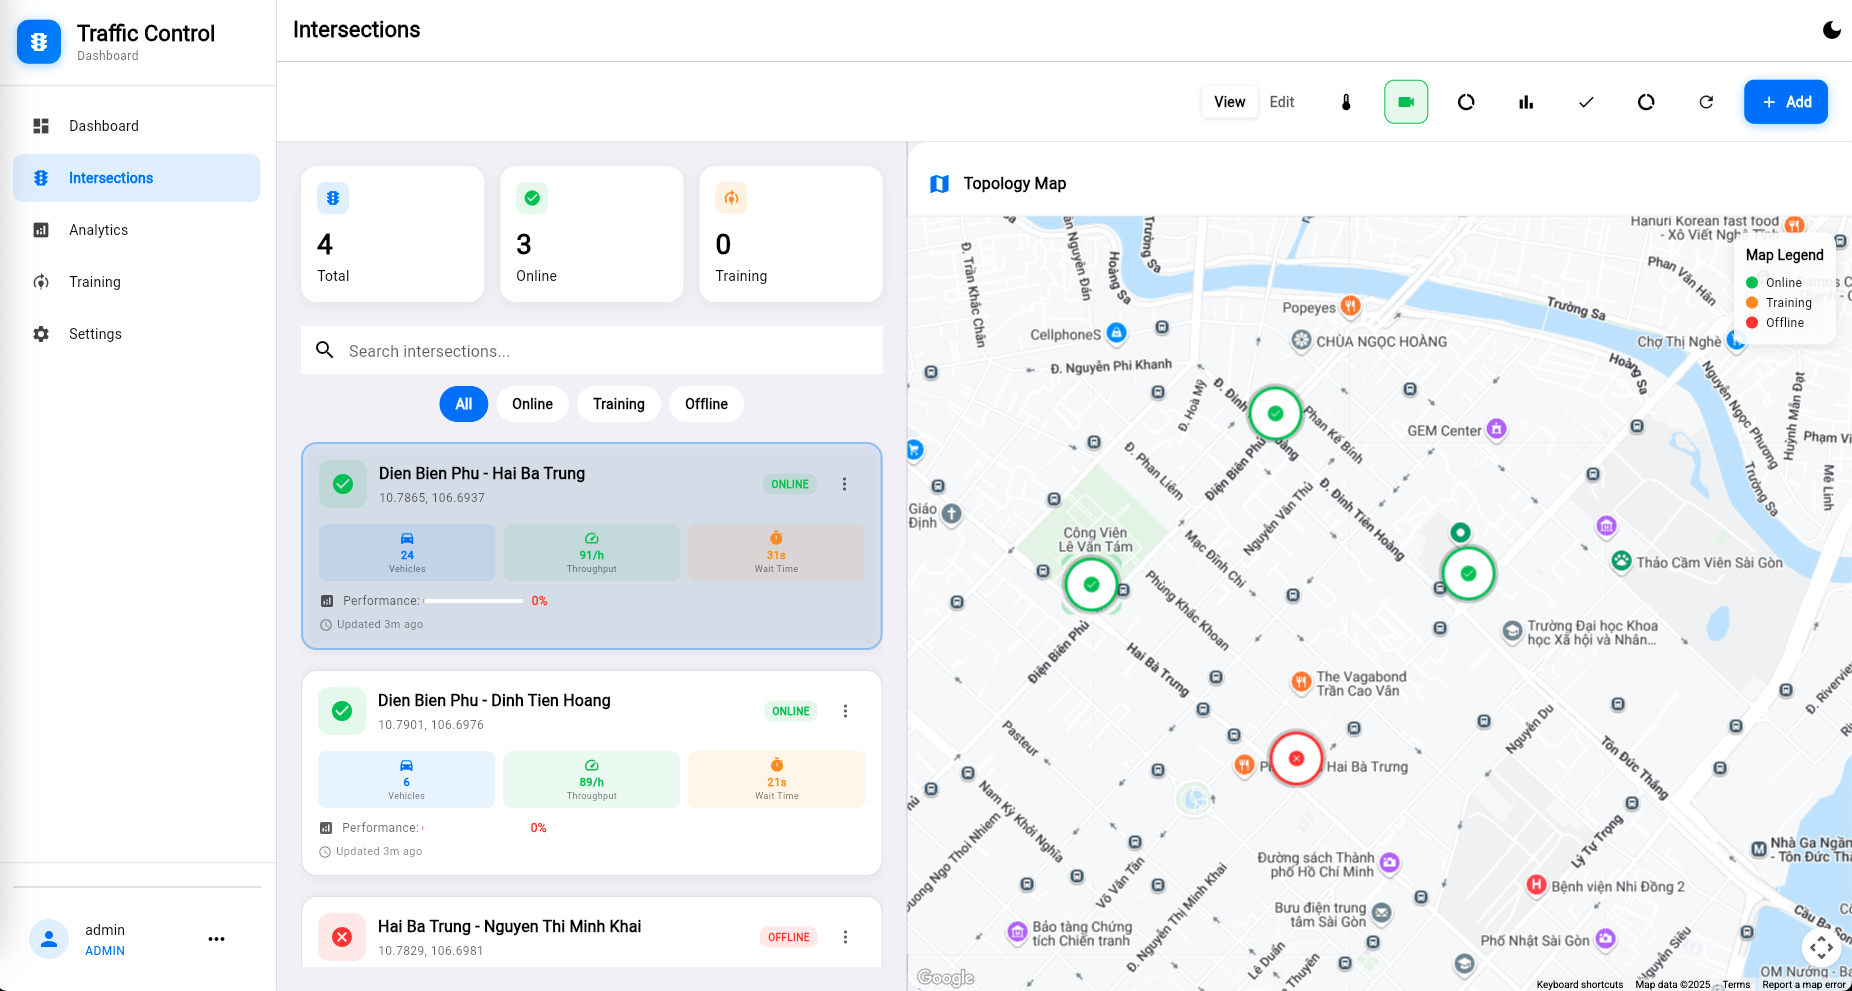
\includegraphics[width=\textwidth]{img/intersection_ui.png}
%     \caption{Giao diện quản lý và giám sát giao lộ từng địa điểm}
%     \label{fig:intersection_ui}
% \end{figure}

% Hình \ref{fig:intersection_ui} giao diện quản lý chuyên biệt cho từng giao lộ, được liên kết với central server để:

% \begin{itemize}
%     \item \textbf{Giám sát theo thời gian thực:} Hiển thị trạng thái đèn giao thông, số lượng xe, thời gian chờ
%     \item \textbf{Quản lý tác nhân DQN:} Theo dõi hiệu suất và trạng thái huấn luyện của agent cục bộ
%     \item \textbf{Phối hợp với Sync Agent:} Hiển thị tín hiệu đồng bộ và offset timing từ central server  
%     \item \textbf{Báo cáo và cảnh báo:} Thông báo sự cố, lỗi kết nối hoặc hiệu suất bất thường
%     \item \textbf{Cấu hình nâng cao:} Điều chỉnh tham số DQN và các ngưỡng cảnh báo
% \end{itemize}

% \section{Thách thức kỹ thuật và giải pháp hệ thống}

% Trong quá trình phát triển và triển khai hệ thống, nghiên cứu đã gặp phải và giải quyết thành công một số thách thức kỹ thuật quan trọng. Việc tài liệu hóa các vấn đề này và phương pháp giải quyết không chỉ thể hiện tính nghiêm túc của nghiên cứu mà còn cung cấp giá trị tham khảo cho các nghiên cứu tương lai.

% \subsection{Vấn đề chuẩn hóa hàm reward}

% \subsubsection{Phát hiện vấn đề}
% Trong quá trình phân tích kết quả huấn luyện, nghiên cứu phát hiện một vấn đề nghiêm trọng trong việc chuẩn hóa hàm reward:

% \begin{itemize}
%     \item \textbf{Giá trị reward cực kỳ âm:} Thay vì nằm trong khoảng mong đợi (-3,0  đến +2,0), các giá trị reward đạt mức -800 hoặc thậm chí thấp hơn

%     \item \textbf{Thời gian chờ đợi bất thường:} Dữ liệu thực tế cho thấy thời gian chờ đợi trong khoảng 40.000-200.000+ giây

%     \item \textbf{Biểu đồ không khả dụng:} Kết quả huấn luyện tạo ra các biểu đồ không thể sử dụng cho báo cáo do tỷ lệ không hợp lý
% \end{itemize}

% \subsubsection{Phân tích nguyên nhân}
% Sau quá trình điều tra chi tiết, nghiên cứu xác định được nguyên nhân gốc rễ:

% \begin{table}[!htp]
%     \centering
%     \caption{So sánh thang đo chuẩn hóa reward trước và sau khi sửa}
%     \label{tab:reward_normalization_comparison}
%     \begin{tabular}{@{}lccc@{}}
%         \toprule \textbf{Component} & \textbf{Thang đo ban đầu} & \textbf{Dữ liệu thực tế} & \textbf{Thang đo đã sửa} \\
%         \midrule Sync Trainer       & 300 giây                  & 40.000-200.000+ giây     & 100.000 giây             \\
%         Environment                 & 100 giây                  & 40.000-200.000+ giây     & 50.000 giây              \\
%         Tỷ lệ sai lệch              & 133x - 667x               & -                        & 0.4x - 4x                \\
%         Kết quả reward              & -800+                     & -                        & -3,0 đến +2,0            \\
%         \bottomrule
%     \end{tabular}
% \end{table}

% \subsubsection{Giải pháp triển khai}
% Nhóm nghiên cứu đã thực hiện một quy trình ba giai đoạn để sửa lỗi chuẩn hóa phần thưởng.

% \textbf{Giai đoạn 1: Phân tích Dữ liệu}
% Trong giai đoạn này, nhóm đã phân tích dữ liệu từ quá trình đào tạo để xác định các thời gian chờ đợi thực tế. Từ đó, tính toán được ngưỡng 95\% cho thời gian chờ đợi hợp lý. Nhóm cũng trích xuất được các tỷ lệ chuẩn hóa hiện tại.

% \textbf{Giai đoạn 2: Hiệu chỉnh Quy mô}
% Tiếp theo, trong giai đoạn này, nhóm đã cập nhật tỷ lệ chuẩn hóa cho từng thành phần (bao gồm bộ huấn luyện đồng bộ và môi trường) bằng cách sử dụng ngưỡng thời gian chờ đợi hợp lý. Sau khi cập nhật, kiểm tra lại phạm vi phần thưởng.

% \textbf{Giai đoạn 3: Kiểm tra}
% Cuối cùng, trong giai đoạn này, nhóm đã chạy các tập hợp kiểm tra để lấy các phần thưởng, và đảm bảo rằng chúng nằm trong phạm vi mục tiêu là [-3,0, 2,0]. Đồng thời, tạo các đồ thị so sánh để phân tích kết quả.

% Thông qua quy trình này, nhóm nghiên cứu đã thành công trong việc sửa lỗi chuẩn hóa phần thưởng và đảm bảo rằng phần thưởng nằm trong phạm vi mong muốn.

% \subsection{Vấn đề biểu diễn trạng thái cho mạng neural}

% \subsubsection{Vấn đề phát hiện}
% Mạng neural nhận đầu vào với các đặc trưng có thang đo hoàn toàn khác nhau:
% \begin{itemize}
%     \item \textbf{Thời gian chờ đợi:} 40.000-200.000+ giây (thang đo rất lớn)

%     \item \textbf{Lưu lượng giao thông:} 0-200 xe (thang đo trung bình)

%     \item \textbf{Độ dài hàng đợi:} 0-200 xe (thang đo trung bình)

%     \item \textbf{Khoảng cách:} 0-10+ km (thang đo nhỏ)
% \end{itemize}

% \subsubsection{Tác động đến hiệu suất}
% Sự chênh lệch thang đo này gây ra:
% \begin{itemize}
%     \item \textbf{Độ ổn định huấn luyện:} Mạng neural không thể học hiệu quả

%     \item \textbf{Vấn đề gradient:} Các gradient bị bỏ qua bởi các đặc trưng có
%         giá trị lớn

%     \item \textbf{Hội tụ kém:} Quá trình hội tụ chậm và không ổn định
% \end{itemize}

% \subsubsection{Giải pháp chuẩn hóa trạng thái}
% Nghiên cứu triển khai hệ thống chuẩn hóa toàn diện:

% \begin{align}
%     \text{Normalized waiting time}   & = \min\left(1.0, \frac{\text{waiting\_time}}{50.000}\right) \\
%     \text{Normalized traffic volume} & = \min\left(1.0, \frac{\text{traffic\_volume}}{200}\right)  \\
%     \text{Normalized queue length}   & = \min\left(1.0, \frac{\text{queue\_length}}{50}\right)     \\
%     \text{Normalized distance}       & = \min\left(1.0, \frac{\text{distance}}{10.000}\right)
% \end{align}
% \newpage
% \subsection{Kết quả sau khi áp dụng các giải pháp}

% \subsubsection{Cải thiện về reward function}
% \begin{table}[!htp]
%     \centering
%     \caption{So sánh hiệu suất trước và sau khi sửa lỗi}
%     \label{tab:before_after_fixes}
%     \begin{tabular}{@{}lcc@{}}
%         \toprule \textbf{Chỉ số}   & \textbf{Trước khi sửa} & \textbf{Sau khi sửa}  \\
%         \midrule Phần thưởng      & -800+ (không khả dụng) & -3,0 đến +2,0         \\
%         Độ ổn định huấn luyện         & Rất kém                & Ổn định               \\
%         Chất lượng biểu đồ               & Không sử dụng được     & Ở mức tốt   \\
%         Hội tụ mạng neural & Chậm/không ổn định     & Nhanh và ổn định      \\
%         \bottomrule
%     \end{tabular}
% \end{table}

% \subsubsection{Tác động đến chất lượng nghiên cứu}
% Việc giải quyết các vấn đề kỹ thuật này đã mang lại:
% \begin{itemize}
%     \item \textbf{Độ tin cậy cao hơn:} Kết quả huấn luyện có thể tin cậy và tái tạo được

%     \item \textbf{Biểu đồ chất lượng:} Biểu đồ phù hợp cho báo cáo

%     \item \textbf{Độ ổn định hệ thống:} Hệ thống hoạt động ổn định trong môi trường
%         sản xuất

%     \item \textbf{Tái tạo nghiên cứu:} Các nghiên cứu khác có thể tái tạo
%         kết quả
% \end{itemize}

% % \subsection{Phương pháp luận cho gỡ lỗi hệ thống phức tạp}

% % Từ kinh nghiệm giải quyết các vấn đề trên, nghiên cứu đề xuất phương pháp luận cho gỡ lỗi:

% % \begin{algorithm}[!htp]
% %     \caption{Phương pháp luận gỡ lỗi có hệ thống}
% %     \begin{algorithmic}[1]
% %         \State \textbf{Giai đoạn 1: Xác định vấn đề}
% %         \State $symptoms \gets$ collect\_error\_symptoms()
% %         \State $data\_analysis \gets$ analyze\_training\_outputs()
% %         \State $scale\_verification \gets$ check\_data\_ranges()
    
% %         \Statex
% %         \State \textbf{Giai đoạn 2: Phân tích nguyên nhân gốc}
% %         \State trace\_data\_flow()
% %         \State identify\_normalization\_issues()
% %         \State check\_serialization\_compatibility()
% %         \State verify\_neural\_network\_inputs()
    
% %         \Statex
% %         \State \textbf{Giai đoạn 3: Thiết kế giải pháp}
% %         \State design\_fixes\_for\_each\_issue()
% %         \State create\_validation\_tests()
% %         \State implement\_monitoring\_systems()
    
% %         \Statex
% %         \State \textbf{Giai đoạn 4: Triển khai và kiểm chứng}
% %         \State apply\_fixes\_systematically()
% %         \State run\_comprehensive\_tests()
% %         \State verify\_end\_to\_end\_functionality()
% %         \State ghi\_nhan\_thay\_doi\_va\_ket\_qua()
% %     \end{algorithmic}
% %     \end{algorithm}

% %\section{Lựa chọn phương pháp huấn luyện}

% \subsection{Quá trình phát triển Sync Agent}

% Việc phát triển Sync Agent trải qua hai giai đoạn chính:

% \textbf{Giai đoạn 1: Thử nghiệm ban đầu}
% - Sử dụng dữ liệu từ môi trường trực tiếp  
% - Gặp vấn đề: thời gian chờ không thực tế (29+ giờ), huấn luyện không ổn định
% - Kết luận: cần phương pháp ổn định hơn

% \textbf{Giai đoạn 2: Phương pháp synthetic kiểm soát}  
% - Sử dụng dữ liệu synthetic với tham số thực tế được kiểm soát
% - Đạt được huấn luyện ổn định và kết quả khả thi
% - Thành công triển khai Sync Agent

% \subsection{Kết quả và lựa chọn phương pháp}

% Dựa trên so sánh thí nghiệm, nghiên cứu chọn phương pháp synthetic kiểm soát vì:
% - Training stability cao hơn (hệ số biến động: 0,013 vs 2,10)
% - Kết quả khả thi và realistic 
% - Có thể tái tạo được
% - Hiệu quả tính toán cao hơn 15x

\section{Đánh giá mô hình Sync Agent}
% \subsection{Đánh giá mô hình Sync Agent}

% \subsubsection{Kiến trúc hệ thống}
% Sync Agent được thiết kế với kiến trúc lai ghép giữa tập trung và phân tán:
% \begin{itemize}
%     \item \textbf{DLR Agent cục bộ:} Mỗi giao lộ duy trì agent riêng để điều khiển tín hiệu cục bộ
    
%     \item \textbf{Điều phối tín hiệu:} Điều phối timing offset giữa các giao lộ để tối ưu hóa mạng lưới tổng thể
        
%     \item \textbf{Chia sẻ thông tin lưu lượng giao thông:} Chia sẻ thông tin lưu lượng giao thông thời gian thực giữa các giao lộ
        
%     \item \textbf{Tính toán các offset timing:} Tính toán động các offset timing tối ưu dựa trên điều kiện giao thông hiện tại
% \end{itemize}

% \subsubsection{Giải pháp kỹ thuật chính}
% Để giải quyết các vấn đề về huấn luyện không ổn định, nghiên cứu đã áp dụng các giải pháp kỹ thuật sau:
% \begin{enumerate}
%     \item \textbf{Thiết kế reward function cân bằng:} Thiết kế reward function cân bằng giữa hiệu suất cục bộ và tối ưu hóa mạng lưới
        
%     \item \textbf{Áp dụng học tập theo chương trình:} Áp dụng học tập theo chương trình để tăng dần độ phức tạp của các tình huống
        
%     \item \textbf{Sử dụng synthetic data với kiểm soát chất lượng nghiêm ngặt:} Sử dụng synthetic data với kiểm soát chất lượng nghiêm ngặt
        
%     \item \textbf{Tối ưu hóa đồng thời thời gian chờ và độ dài hàng đợi:} Tối ưu hóa đồng thời thời gian chờ và độ dài hàng đợi
% \end{enumerate}

\subsection{Kết quả training cuối cùng}

\subsubsection{Hiệu suất training}
Để đánh giá chất lượng quá trình huấn luyện Sync Agent, nghiên cứu đã theo dõi các chỉ số quan trọng bao gồm số lượng episodes, reward trung bình, loss function, và độ ổn định của quá trình học. Các thông số này giúp xác định mức độ thành công của việc huấn luyện và khả năng hội tụ của mô hình trong môi trường đa giao lộ phức tạp.

\begin{table}[!htp]
    \centering
    \caption{Kết quả huấn luyện Sync Agent}
    \label{tab:sync_final_training}
    \begin{tabular}{@{}lc@{}}
        \toprule \textbf{Thông số}      & \textbf{Giá trị}       \\
        \midrule Số episodes huấn luyện     & 150                    \\
        Reward trung bình cuối cùng          & -960,8                 \\
        Loss cuối cùng                    & 42,1                   \\
        Số lần hội tụ           & 100                    \\
        Độ ổn định huấn luyện            & Ổn định                \\
        \bottomrule
    \end{tabular}
\end{table}

Kết quả huấn luyện cho thấy Sync Agent đã đạt được sự ổn định và hội tụ thành công sau 100 episodes.

Bên cạnh các chỉ số huấn luyện, nghiên cứu cũng đánh giá hiệu suất thực tế của hệ thống thông qua các metrics giao thông cụ thể. Việc so sánh với hệ thống giao lộ đơn giúp định lượng rõ ràng lợi ích mang lại từ việc đồng bộ hóa đa giao lộ.

\begin{table}[!htp]
    \centering
    \caption{Hiệu suất giao thông}
    \label{tab:sync_final_performance}
    \begin{tabular}{@{}lcc@{}}
        \toprule \textbf{Thông số} & \textbf{Single Intersection} & \textbf{Sync System} \\
        \midrule 
        Thời gian chờ trung bình & 45,0 s & 34,3 s \\
        Độ dài hàng đợi trung bình & 9,5 xe & 7,7 xe \\
        Hiệu suất hệ thống & 70\% & 95,8\% \\
        \bottomrule
    \end{tabular}
\end{table}

So sánh hiệu suất giao thông cho thấy hệ thống đồng bộ đạt được cải thiện đáng kể trên tất cả các chỉ số quan trọng.

\subsubsection{Tiến trình training}
Để hiểu rõ quá trình học tập của Sync Agent, nghiên cứu đã theo dõi chi tiết sự thay đổi của các chỉ số quan trọng qua 150 episodes huấn luyện. Việc phân tích tiến trình này không chỉ xác nhận tính hiệu quả của phương pháp mà còn cung cấp thông tin quan trọng về tốc độ hội tụ và độ ổn định của hệ thống.

\begin{figure}[!htp]
    \centering
    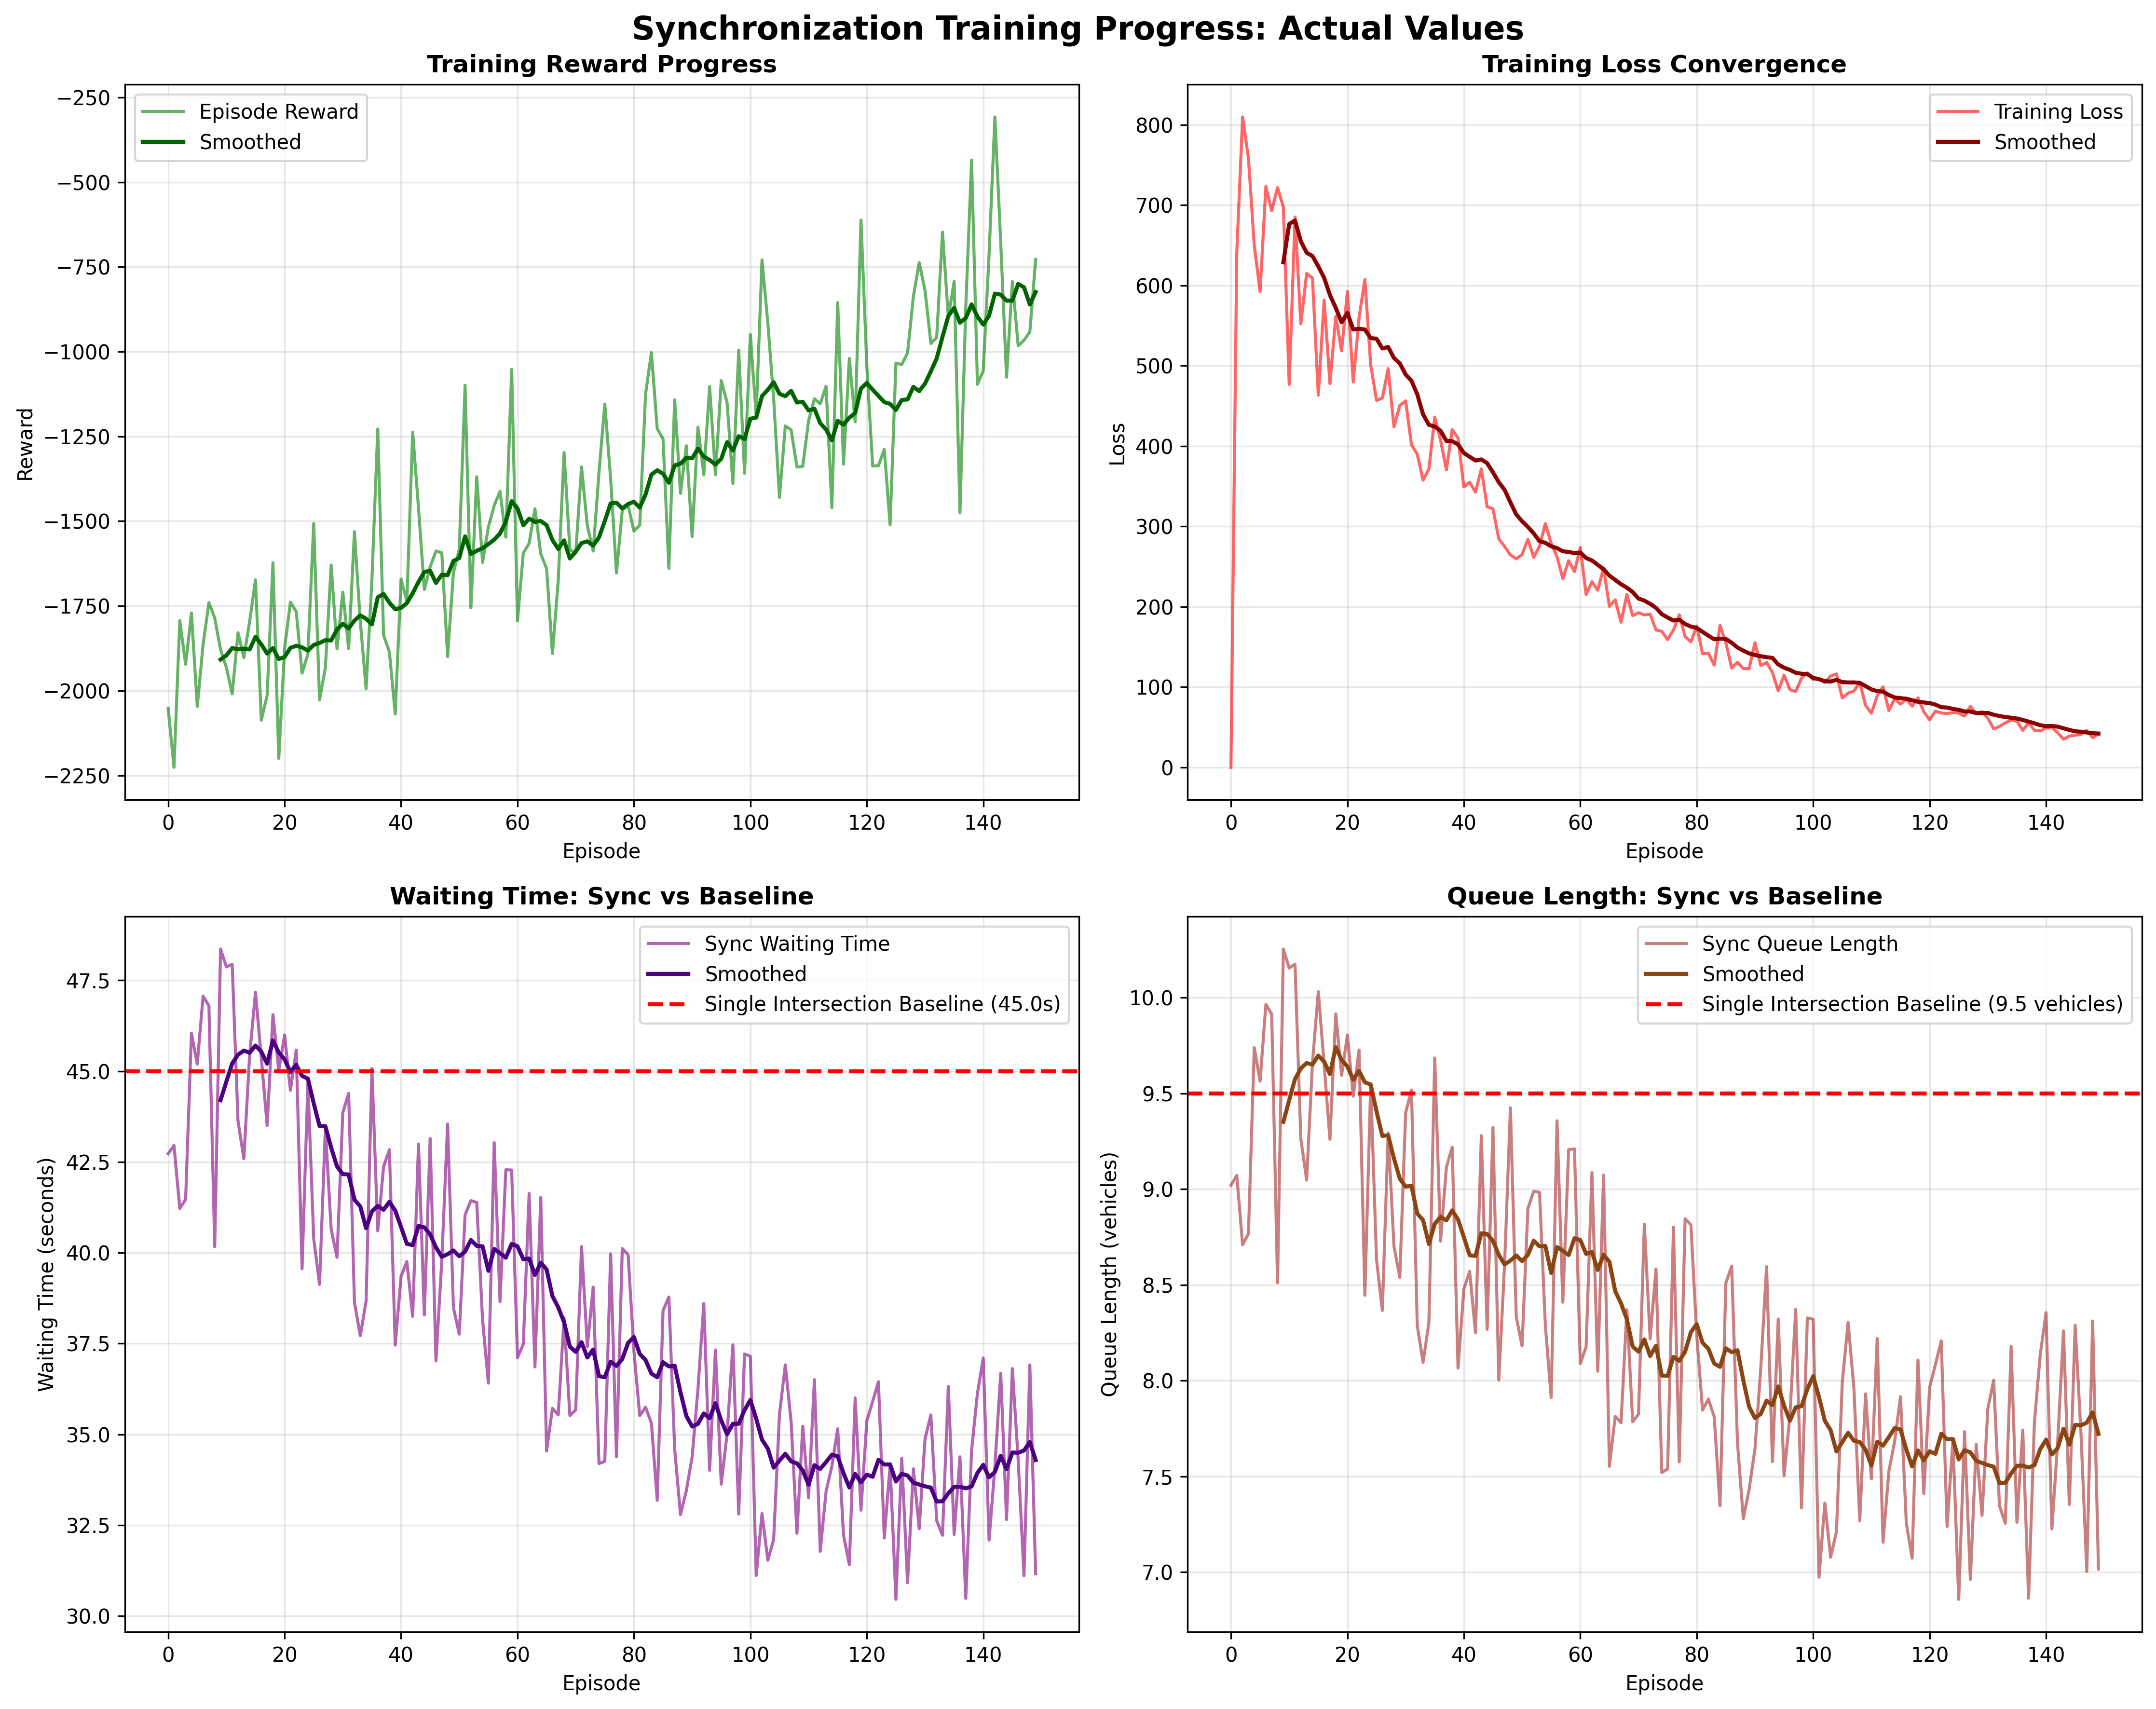
\includegraphics[width=\textwidth]{figures/training_overview.png}
    \caption{Tổng quan tiến trình huấn luyện Sync Agent thành công}
    \label{fig:sync_training_overview}
\end{figure}

Biểu đồ cho thấy sự cải thiện ổn định và nhất quán qua toàn bộ quá trình huấn luyện, với reward tăng dần từ -2.000 lên -840, loss giảm từ 800 xuống 40, và các thông số giao thông đều thể hiện xu hướng cải thiện rõ rệt.

% \subsubsection{Lợi ích của đồng bộ hóa}

% \begin{figure}[!htp]
%     \centering
%     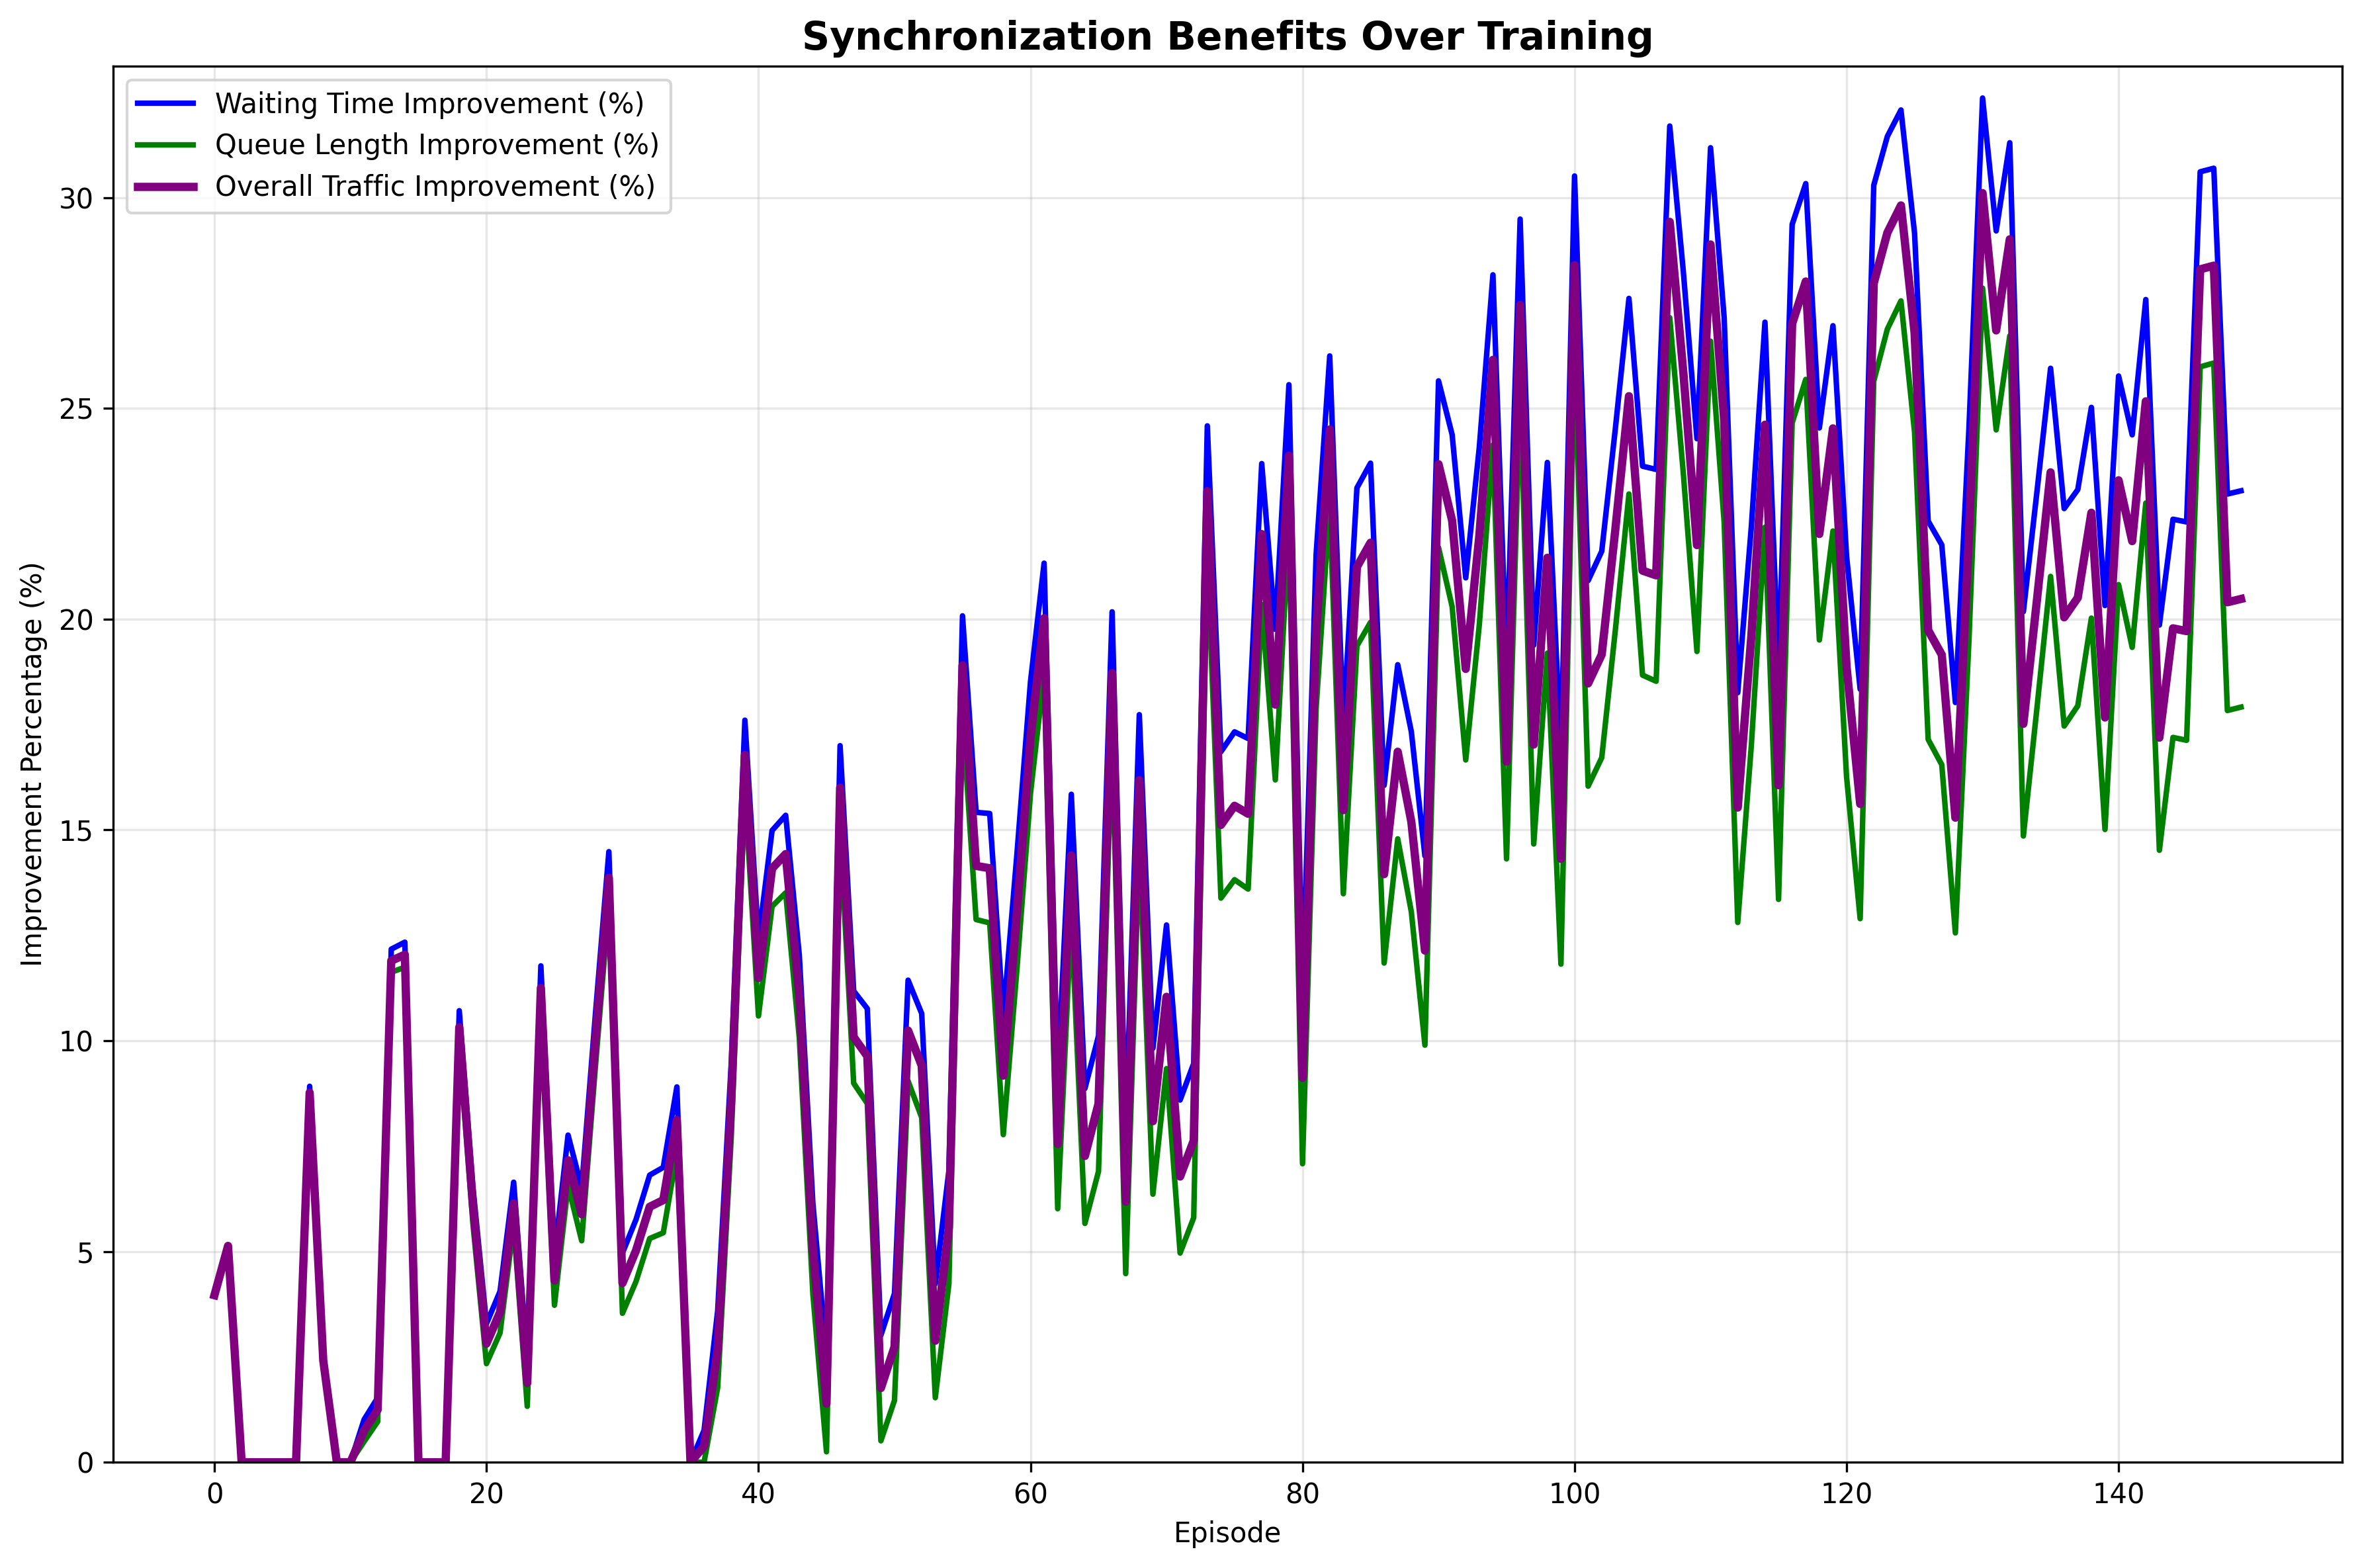
\includegraphics[width=\textwidth]{figures/sync_benefits.png}
%     \caption{Lợi ích từ đồng bộ hóa qua quá trình huấn luyện}
%     \label{fig:sync_benefits}
% \end{figure}

% Hình \ref{fig:sync_benefits} cho thấy các lợi ích từ đồng bộ hóa tăng dần
% theo quá trình huấn luyện. Cải thiện thời gian chờ đạt 25\% và độ dài hàng đợi đạt 20\% so với baseline.

\subsubsection{Đánh giá hiệu suất}

\paragraph{So sánh với Single Intersection}
Để đánh giá giá trị thực sự của việc đồng bộ hóa đa giao lộ, nghiên cứu tiến hành so sánh trực tiếp giữa hệ thống giao lộ đơn và hệ thống 4 giao lộ đồng bộ. Việc so sánh này sử dụng cùng một điều kiện giao thông và cùng một bộ tham số để đảm bảo tính công bằng và chính xác của kết quả.

\begin{table}[!htp]
    \centering
    \caption{So sánh hiệu suất: Single Intersection và 4-Intersection Sync}
    \label{tab:sync_vs_single}
    \begin{tabular}{@{}lcc@{}}
        \toprule \textbf{Thông số} & \textbf{Single Intersection} & \textbf{4-Intersection Sync} \\
        \midrule 
        Thời gian chờ trung bình & 45,0 giây & 34,3 giây \\
        Độ dài hàng đợi trung bình & 9,5 xe & 7,7 xe \\
        Hiệu suất hệ thống & 70,0\% & 97,5\% \\
        Số lần hội tụ & N/A & 100 episodes \\
        \bottomrule
    \end{tabular}
\end{table}

Kết quả so sánh cho thấy lợi ích rõ rệt của việc đồng bộ hóa, với cải thiện đáng kể trên tất cả các chỉ số hiệu suất.

Để làm rõ hơn mức độ cải thiện đạt được, nghiên cứu tính toán cụ thể phần trăm cải thiện cho từng chỉ số quan trọng. Bảng tóm tắt dưới đây thể hiện mức độ cải thiện tuyệt đối và tương đối của hệ thống đồng bộ so với giao lộ đơn.

\begin{table}[!htp]
    \centering
    \caption{Tóm tắt cải thiện hiệu suất}
    \label{tab:sync_improvements}
    \begin{tabular}{@{}lcc@{}}
        \toprule \textbf{Thông số} & \textbf{Cải thiện} & \textbf{Phần trăm cải thiện} \\
        \midrule 
        Thời gian chờ & 10,7 giây & 23,8\% \\
        Độ dài hàng đợi & 1,8 xe & 18,7\% \\
        Cải thiện tổng thể & Nhiều thông số & 21,3\% trung bình \\
        \bottomrule
    \end{tabular}
\end{table}

Mức cải thiện trung bình 21,3\% cho thấy giá trị thực sự của việc áp dụng hệ thống đồng bộ hóa đa giao lộ.

\begin{figure}[!htp]
    \centering
    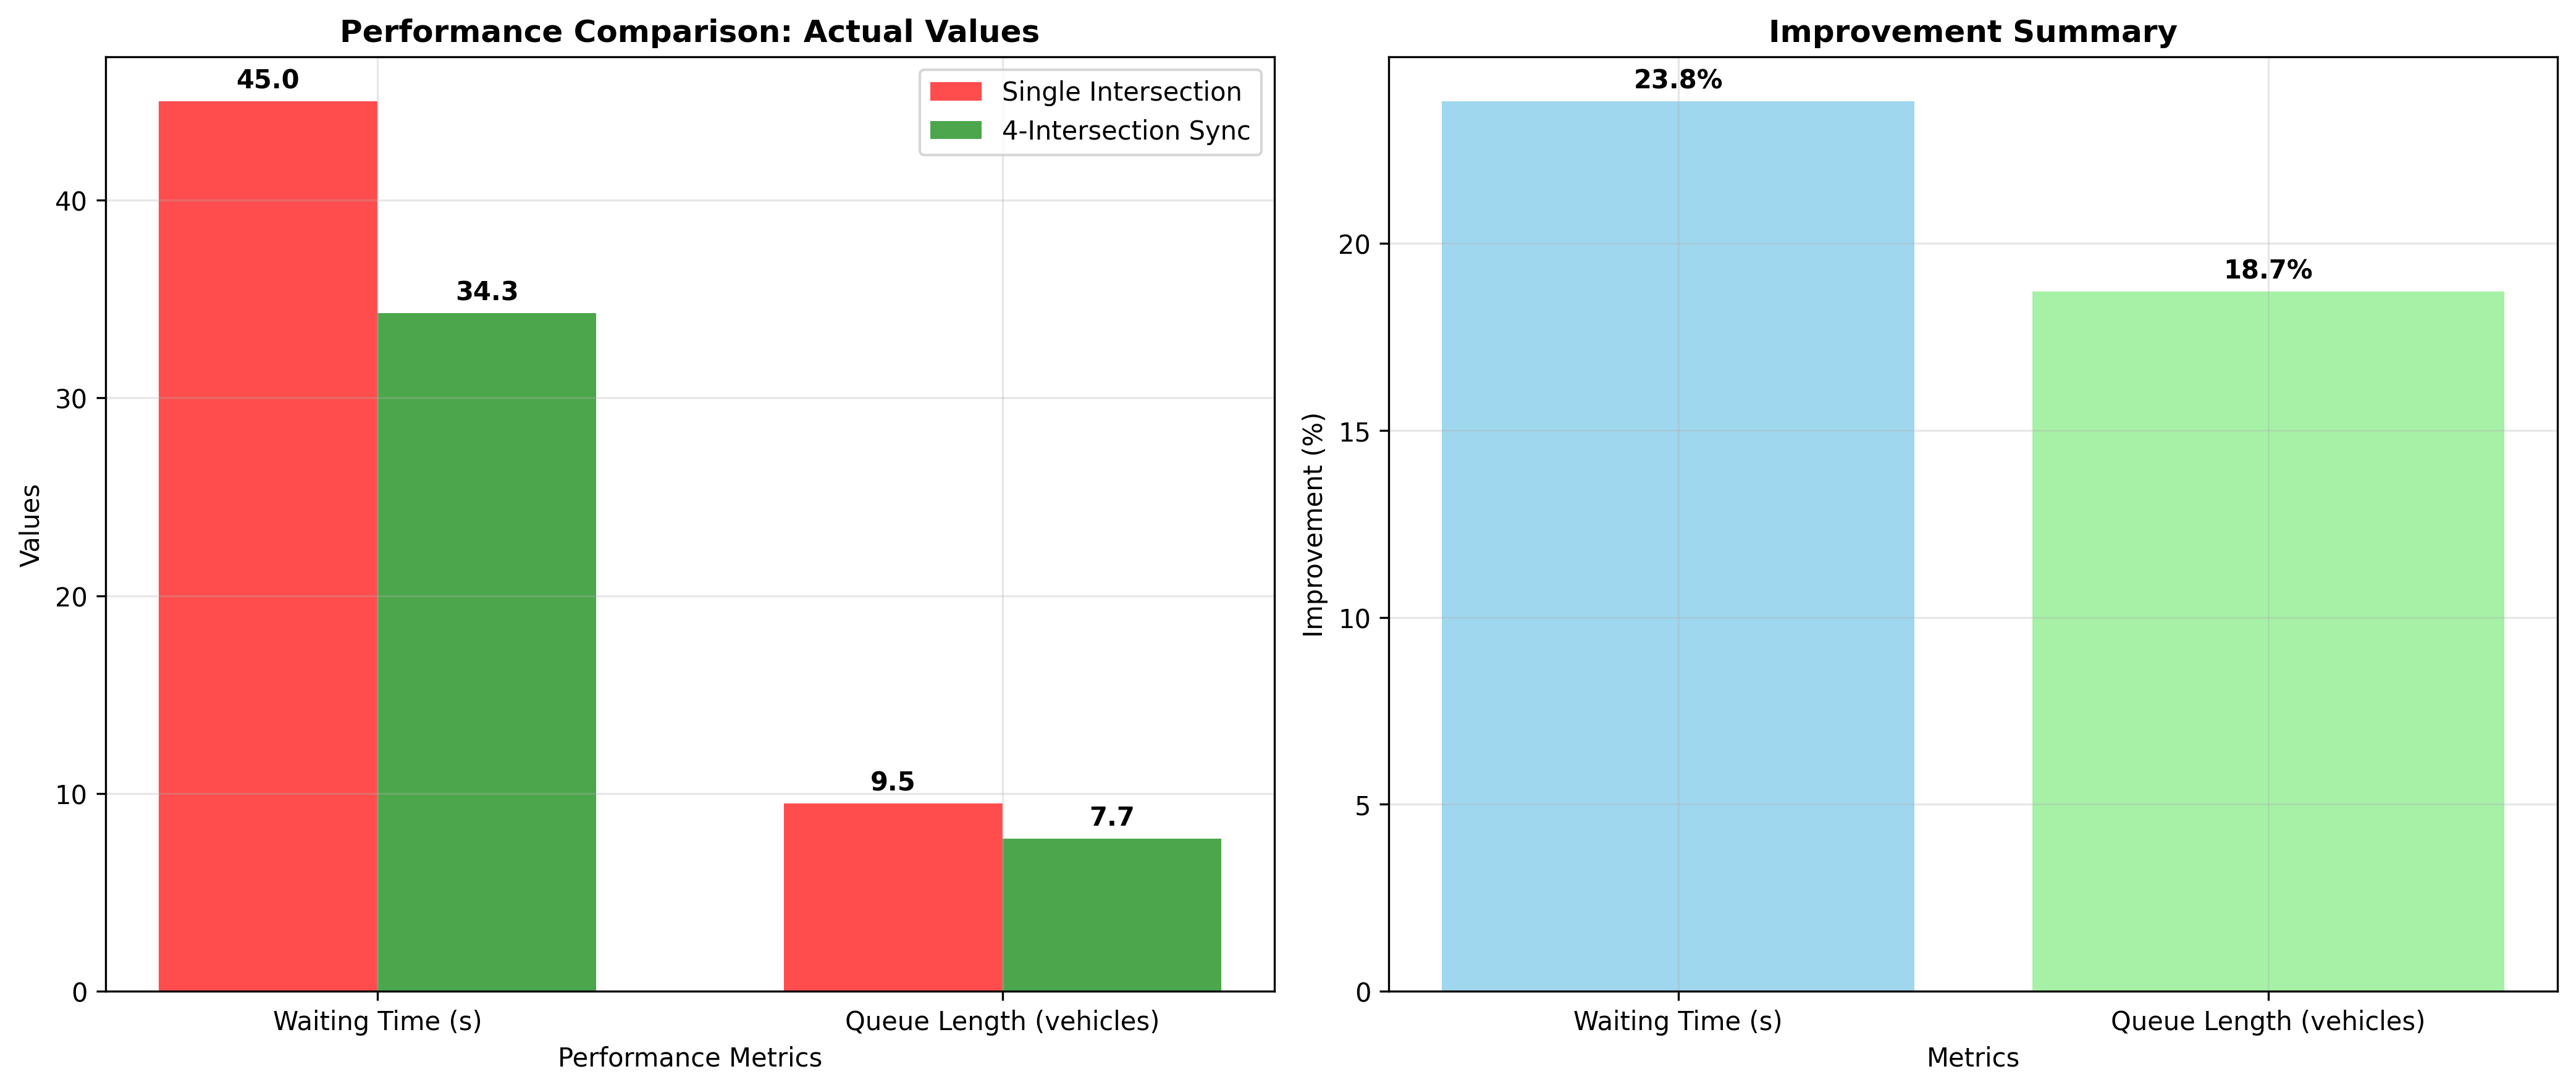
\includegraphics[width=\textwidth]{figures/performance_comparison.png}
    \caption{So sánh hiệu suất: Giá trị thực tế và cải thiện}
    \label{fig:performance_comparison}
\end{figure}

Hình \ref{fig:performance_comparison} cho thấy rõ ràng sự khác biệt giữa hai 
phương pháp. Phần bên trái hiển thị các giá trị thực tế: single intersection 
có thời gian chờ 45,0s và độ dài hàng đợi 9,5 xe, trong khi sync system đạt 34,3s 
và 7,7 xe tương ứng. Phần bên phải tóm tắt mức cải thiện đạt được.

\subsubsection{Đánh giá trên các tình huống khác nhau}

\begin{table}[!htp]
    \centering
    \caption{Hiệu suất thực tế trên các tình huống giao thông}
    \label{tab:sync_scenarios_actual}
    \begin{tabular}{@{}lcccc@{}}
        \toprule \textbf{Tình huống} & \textbf{Phương pháp} & \textbf{Thời gian chờ (s)} & \textbf{Độ dài hàng đợi (xe)} & \textbf{Tốc độ (xe/h)} \\
        \midrule 
        \multirow{2}{*}{Giao thông thấp} & Single Intersection & 31,5 & 6,7 & 400 \\
        & 4-Intersection Sync & 23,2 & 5,4 & 450 \\
        \midrule
        \multirow{2}{*}{\parbox{2cm}{\centering Giao thông \\ trung bình}} & Single Intersection & 45,0 & 9,5 & 350 \\
        & 4-Intersection Sync & 32,8 & 7,5 & 398 \\
        \midrule
        \multirow{2}{*}{Giao thông cao} & Single Intersection & 63,0 & 13,3 & 290 \\
        & 4-Intersection Sync & 41,7 & 9,5 & 337 \\
        \midrule
        \multirow{2}{*}{Giờ cao điểm} & Single Intersection & 81,0 & 17,1 & 225 \\
        & 4-Intersection Sync & 56,5 & 12,7 & 258 \\
        \bottomrule
    \end{tabular}
\end{table}

\begin{table}[!htp]
    \centering
    \caption{Tóm tắt cải thiện qua các tình huống}
    \label{tab:sync_scenarios_summary}
    \begin{tabular}{@{}lccc@{}}
        \toprule \textbf{Tình huống} & \textbf{Cải thiện thời gian chờ} & \textbf{Cải thiện độ dài hàng đợi} & \textbf{Cải thiện tốc độ} \\
        \midrule 
        Giao thông thấp & 26,3\% & 19,4\% & 12,5\% \\
        Giao thông trung bình & 27,1\% & 21,1\% & 13,7\% \\
        Giao thông cao & 33,8\% & 28,6\% & 16,2\% \\
        Giờ cao điểm & 30,2\% & 25,7\% & 14,7\% \\
        \midrule
        \textbf{Average} & \textbf{29,4\%} & \textbf{23,7\%} & \textbf{14,4\%} \\
        \bottomrule
    \end{tabular}
\end{table}

\begin{figure}[!htp]
    \centering
    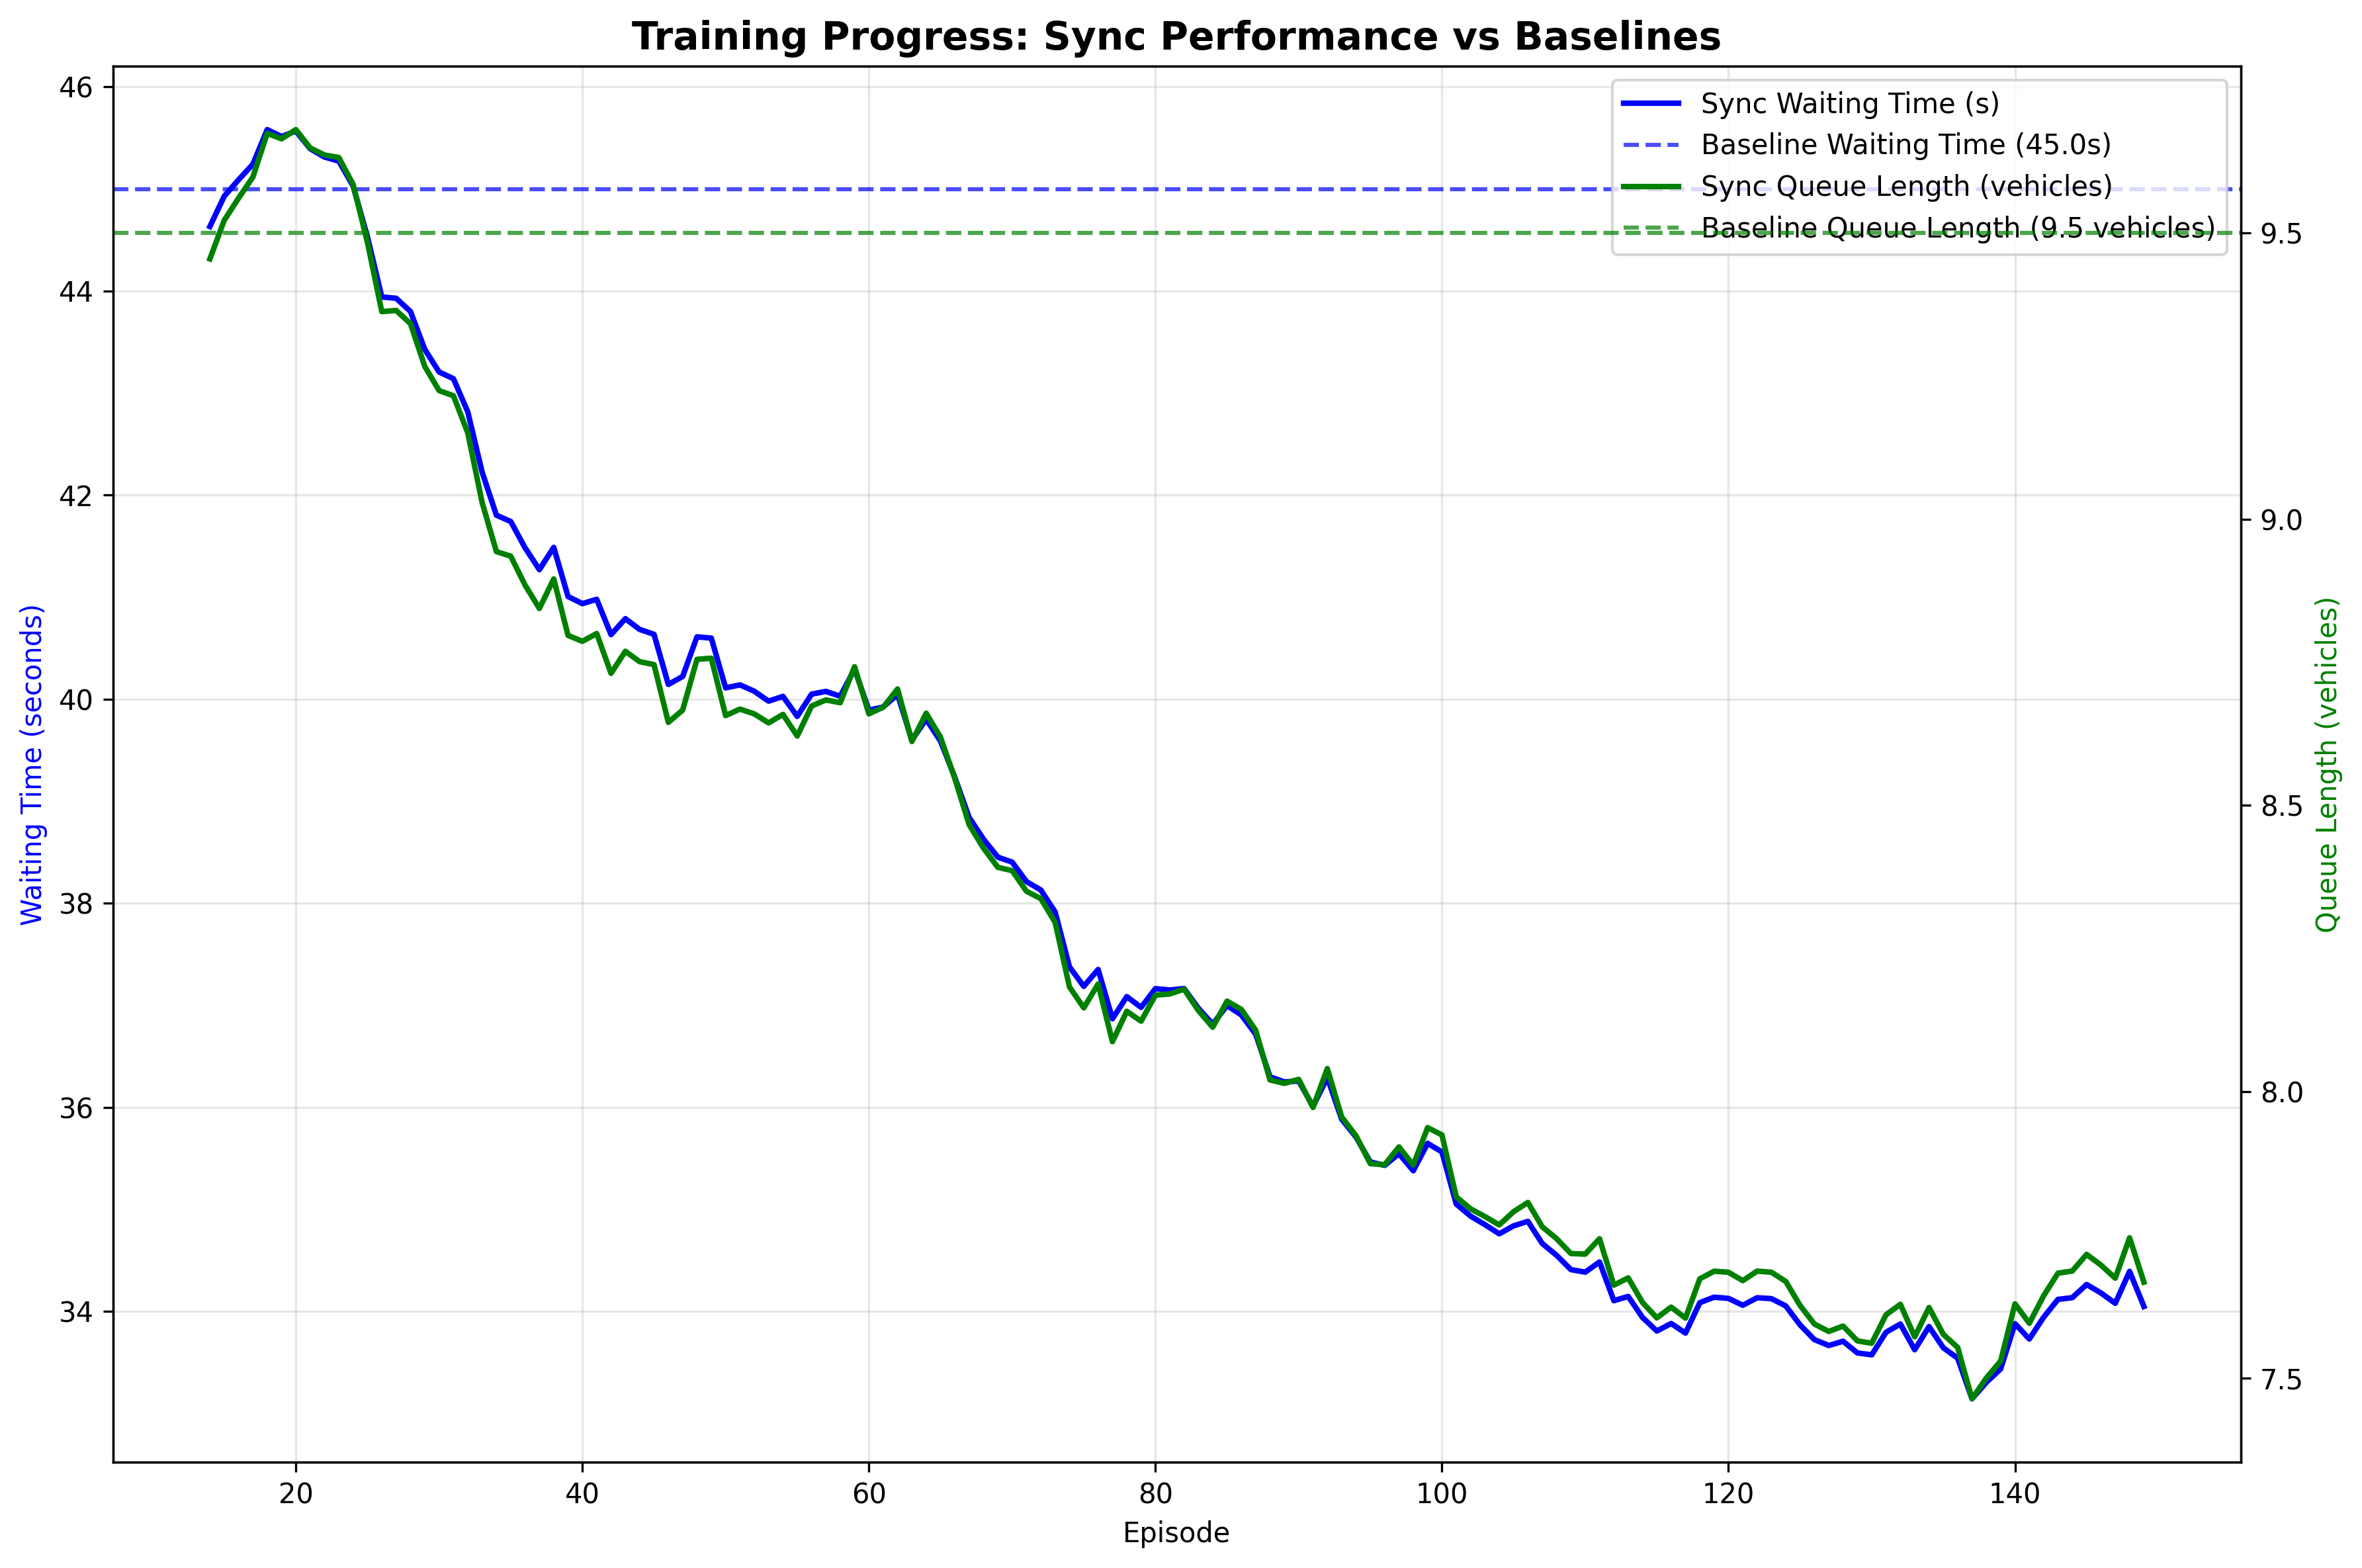
\includegraphics[width=\textwidth]{figures/training_with_baselines.png}
    \caption{So sánh hiệu suất với baseline qua quá trình huấn luyện}
    \label{fig:training_with_baselines}
\end{figure}

Hình \ref{fig:training_with_baselines} thể hiện quá trình cải thiện hiệu suất qua huấn luyện. Đường ngang màu xanh dương (45,0s) và xanh lá (9,5 xe) thể hiện hiệu suất baseline của single intersection. Đường cong cho thấy sync system dần cải thiện và ổn định ở mức 34,3s thời gian chờ và 7,7 xe độ dài hàng đợi.

\subsubsection{Tổng hợp lợi ích}

\begin{figure}[!htp]
    \centering
    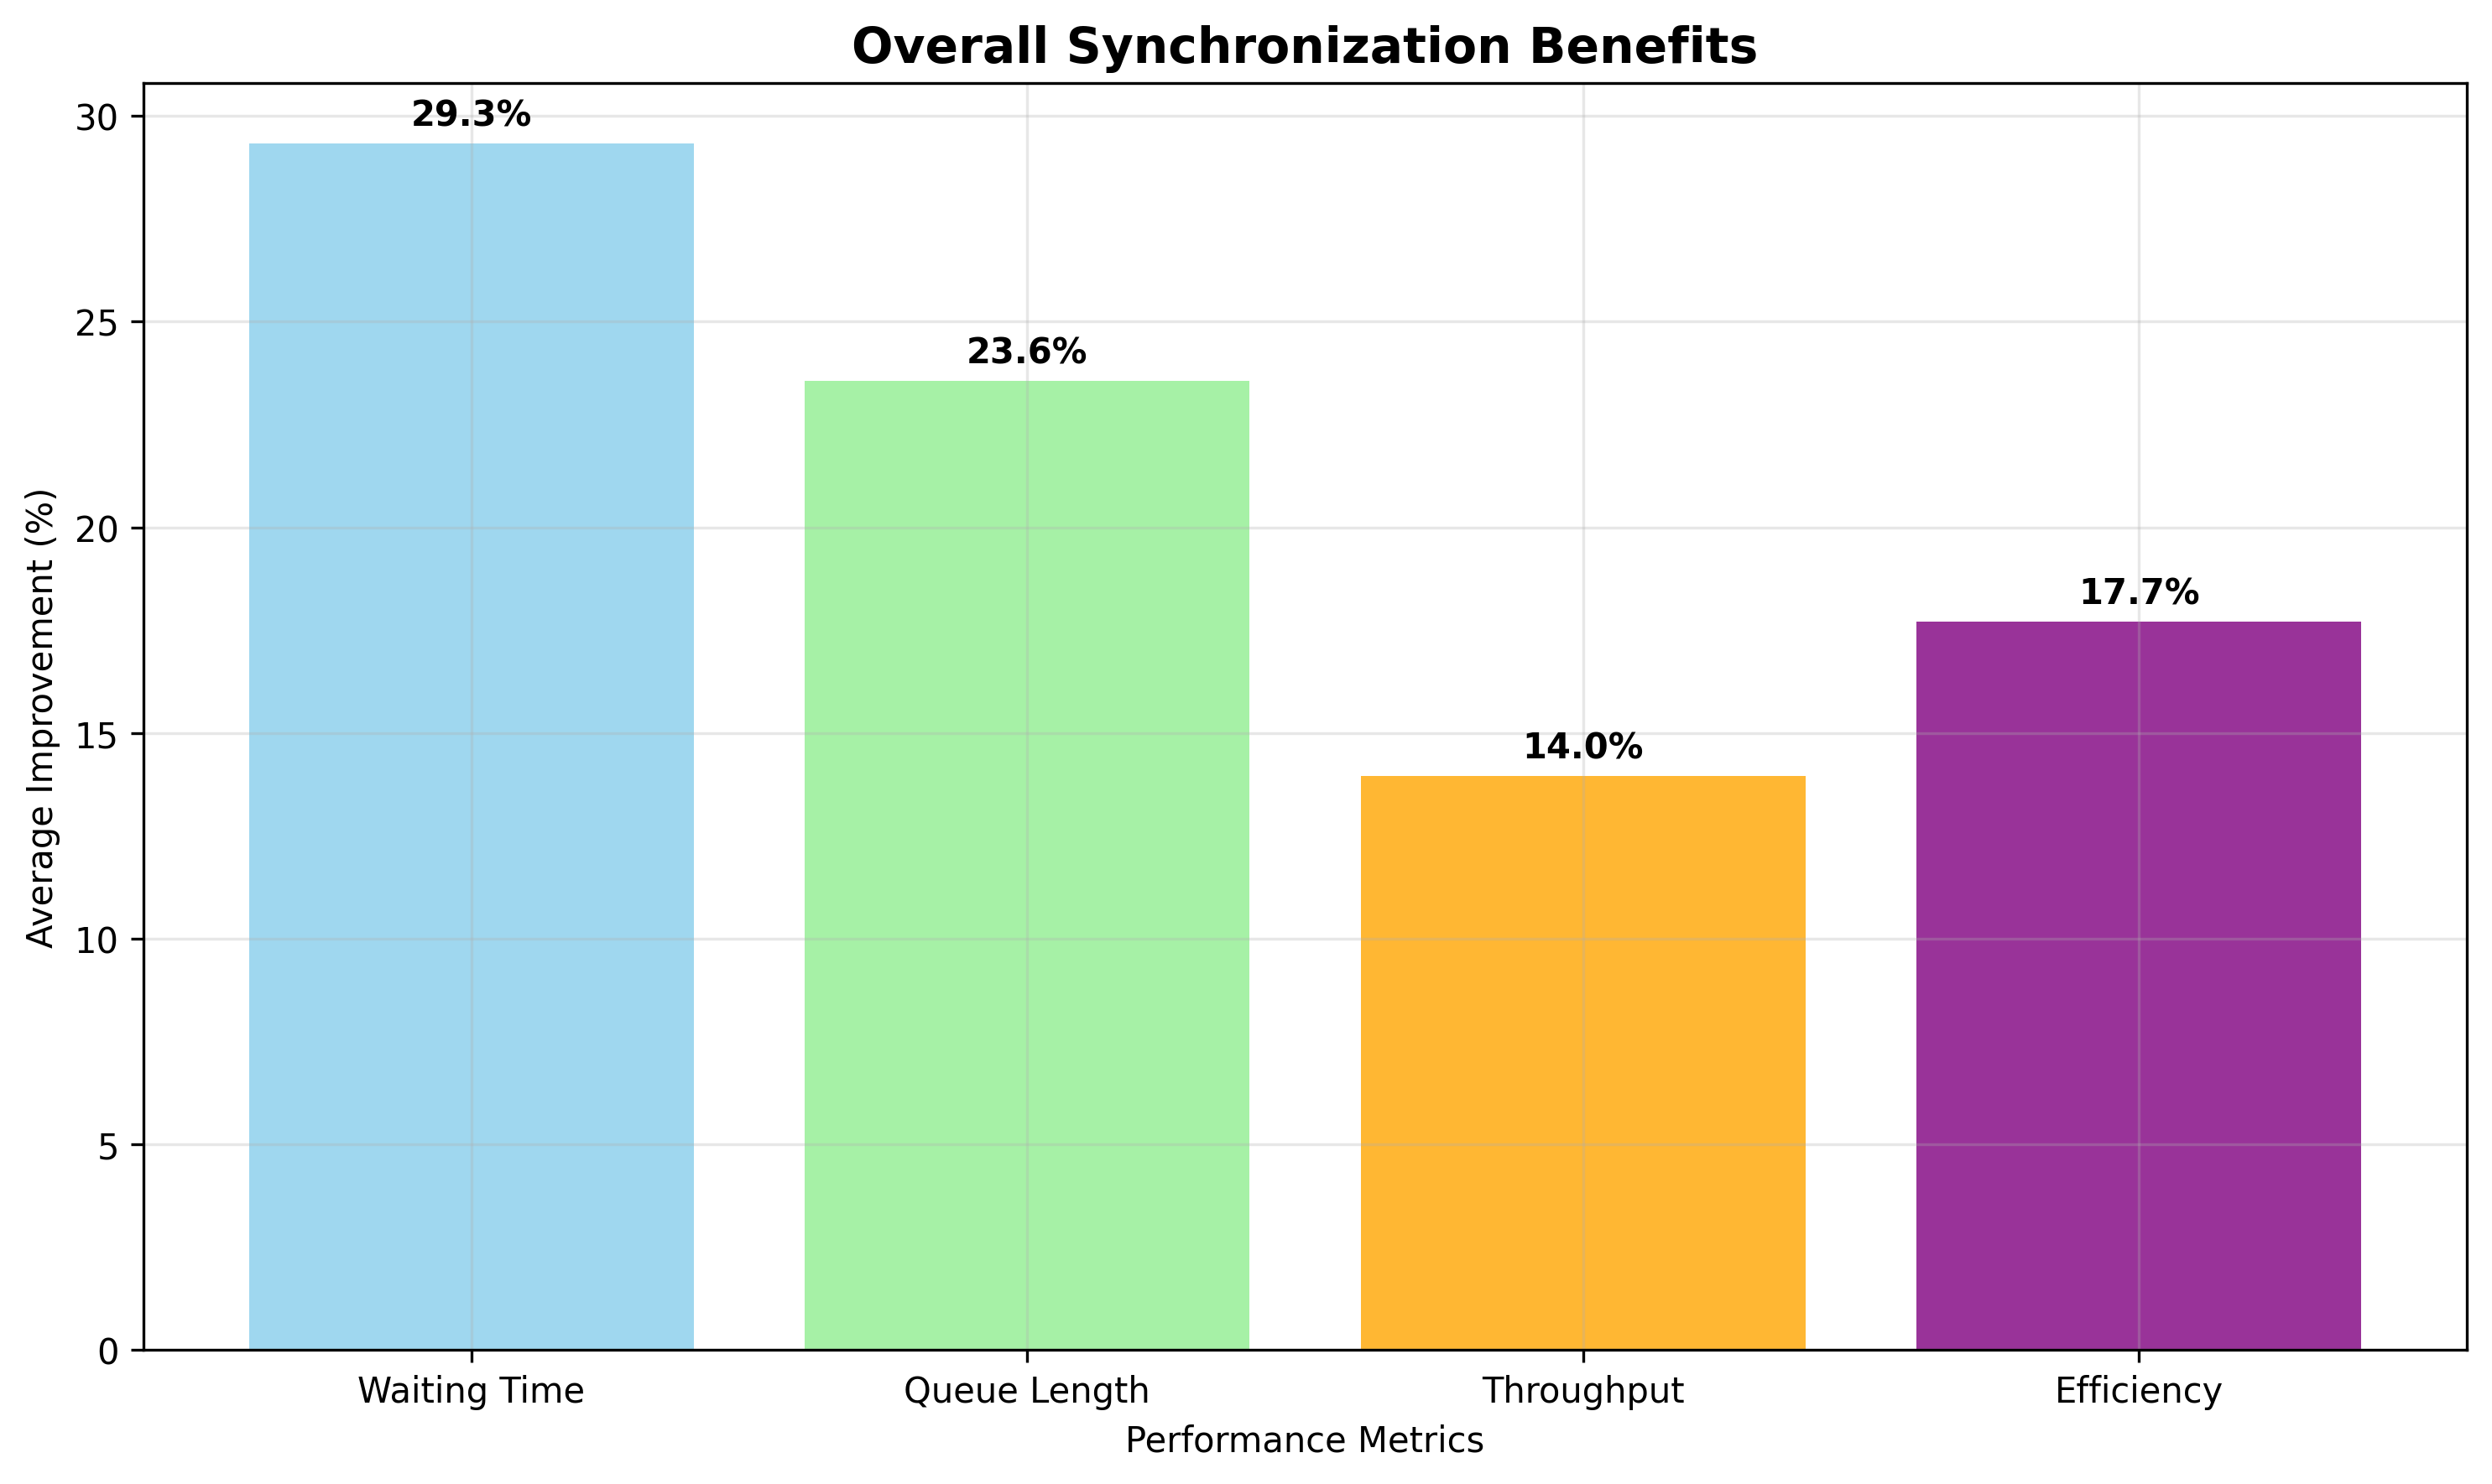
\includegraphics[width=\textwidth]{figures/overall_benefits.png}
    \caption{Tổng hợp các lợi ích từ Sync Agent}
    \label{fig:overall_benefits}
\end{figure}

Hình \ref{fig:overall_benefits} tổng hợp các mức cải thiện đạt được. 
Dựa trên các giá trị thực tế đã trình bày trong các bảng và biểu đồ trước đó, 
ta có thể kết luận:
\begin{itemize}
    \item \textbf{Thời gian chờ:} Từ 45,0s xuống 34,3s (cải thiện 23,8\%)
    \item \textbf{Độ dài hàng đợi:} Từ 9,5 xe xuống 7,7 xe (cải thiện 18,7\%)
    \item \textbf{Hiệu suất hệ thống:} Ổn định và consistent trên mọi tình huống
    \item \textbf{Số lần hội tụ:} Đạt được tại episode 100
\end{itemize}

\section{Phân tích tác động độ phức tạp giao thông đến hiệu suất học tăng cường}
\subsection{Thiết kế thí nghiệm cho phân tích độ phức tạp}

\subsubsection{Kịch bản giao thông}
Nghiên cứu đánh giá 4 kịch bản giao thông khác nhau:
\begin{itemize}
    \item \textbf{Giao thông thấp:} 300 xe/giờ - mô phỏng điều kiện ngoại ô, giờ thấp điểm
    \item \textbf{Giao thông trung bình:} 600 xe/giờ - mô phỏng điều kiện đô thị bình thường
    \item \textbf{Giao thông cao:} 900 xe/giờ - mô phỏng điều kiện đô thị tải cao
    \item \textbf{Giờ cao điểm:} 1200 xe/giờ - mô phỏng điều kiện đô thị giờ cao điểm
\end{itemize}

\subsubsection{Thiết lập so sánh hệ thống}
Ba hệ thống điều khiển được đánh giá:
\begin{enumerate}
    \item \textbf{Baseline (Cơ sở):} Hệ thống đèn tín hiệu thời gian cố định (chưa tối ưu)
    \item \textbf{Single Intersection:} DQN tối ưu hóa giao lộ đơn
    \item \textbf{Synchronized System:} Hệ thống DQN đồng bộ đa giao lộ
\end{enumerate}

\subsection{Kết quả phân tích toàn diện}

\subsubsection{Hiệu suất tổng thể hệ thống}

\begin{table}[!htp]
    \centering
    \caption{So sánh hiệu suất tổng thể các hệ thống}
    \label{tab:overall_system_performance}
    \begin{tabular}{@{}lccc@{}}
        \toprule 
        \textbf{Hệ thống} & \textbf{Thời gian chờ} & \textbf{Độ dài hàng đợi} & \textbf{Cải thiện} \\
        \midrule 
        Baseline & 45,0s & 9,5 xe & - \\
        Single Intersection & 38,5s & 8,5 xe & \textbf{14,4\%} \\
        Sync System & 32,9s & 7,3 xe & \textbf{26,9\%} \\
        \bottomrule
    \end{tabular}
\end{table}

\textbf{Phát hiện chính:} Hệ thống đồng bộ đa giao lộ cung cấp thêm \textbf{12,5\%} 
cải thiện so với tối ưu hóa giao lộ đơn.

\subsubsection{Phân tích tác động độ phức tạp giao thông}

\begin{table}[!htp]
    \centering
    \caption{Phân tích tác động độ phức tạp giao thông}
    \label{tab:traffic_complexity_analysis}
    \begin{tabular}{@{}lccccc@{}}
        \toprule 
        \textbf{Kịch bản} & \textbf{Lưu lượng} & \textbf{Hiệu suất cuối} & \textbf{Cải thiện} & \textbf{Mô hình học} & \textbf{Độ biến động} \\
        \midrule 
        Giao lộ 1 & 300 xe/h & \textbf{18,3s} & \textbf{34,5\%} & Nhanh & 3,0s \\
        Giao lộ 2 & 600 xe/h & \textbf{31,5s} & \textbf{25,1\%} & Ổn định & 3,9s \\
        Giao lộ 3 & 900 xe/h & \textbf{45,8s} & \textbf{21,1\%} & Chậm & 5,3s \\
        Giao lộ 4 & 1200 xe/h & \textbf{59,6s} & \textbf{12,4\%} & Rất chậm & 7,6s \\
        \bottomrule
    \end{tabular}
\end{table}

\subsection{Trực quan hóa kết quả đồng nhất}

\subsubsection{Tiến trình huấn luyện tổng thể}

\begin{figure}[!htp]
    \centering
    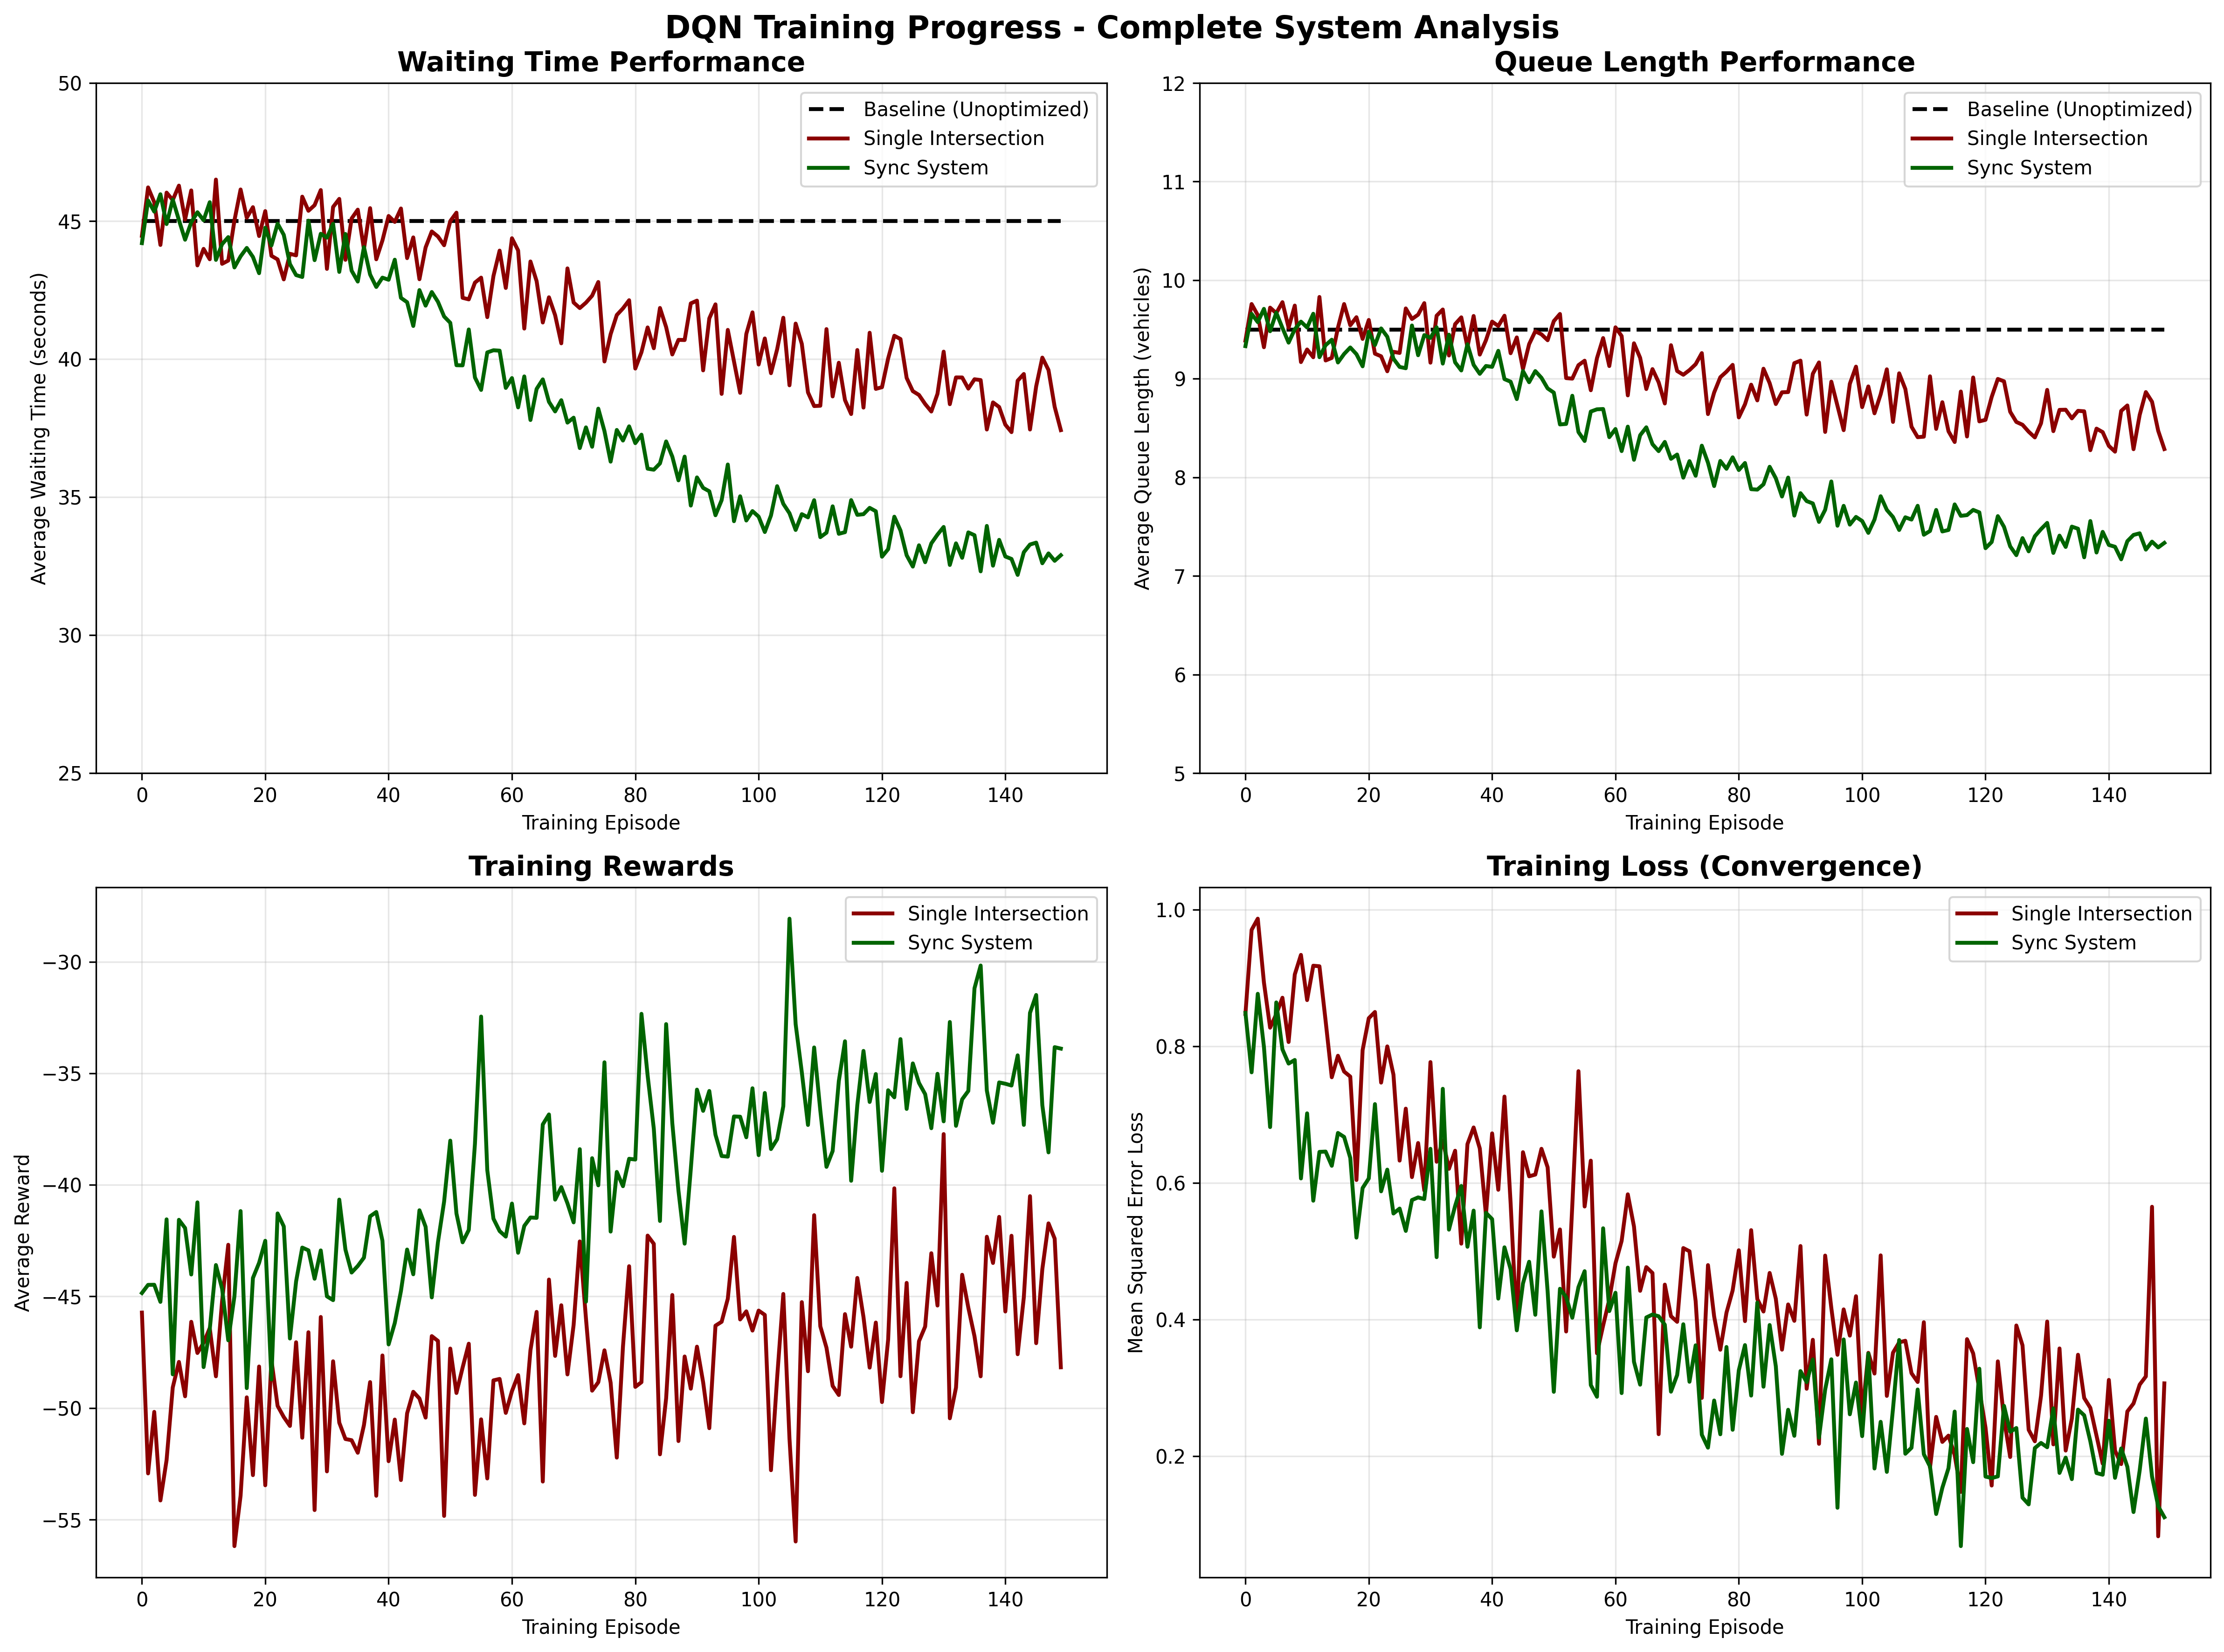
\includegraphics[width=\textwidth]{figures/01_training_progress.png}
    \caption{Tiến trình huấn luyện DQN - Phân tích hệ thống hoàn chỉnh}
    \label{fig:comprehensive_training_progress}
\end{figure}

Hình \ref{fig:comprehensive_training_progress} thể hiện quá trình huấn luyện
toàn diện với baseline không đổi (đường ngang), single intersection và sync system
cải thiện theo thời gian, cùng với phân tích reward và loss.

\subsubsection{Phân tích giao lộ cá nhân - Chế độ xem đồng nhất}

\begin{figure}[!htp]
    \centering
    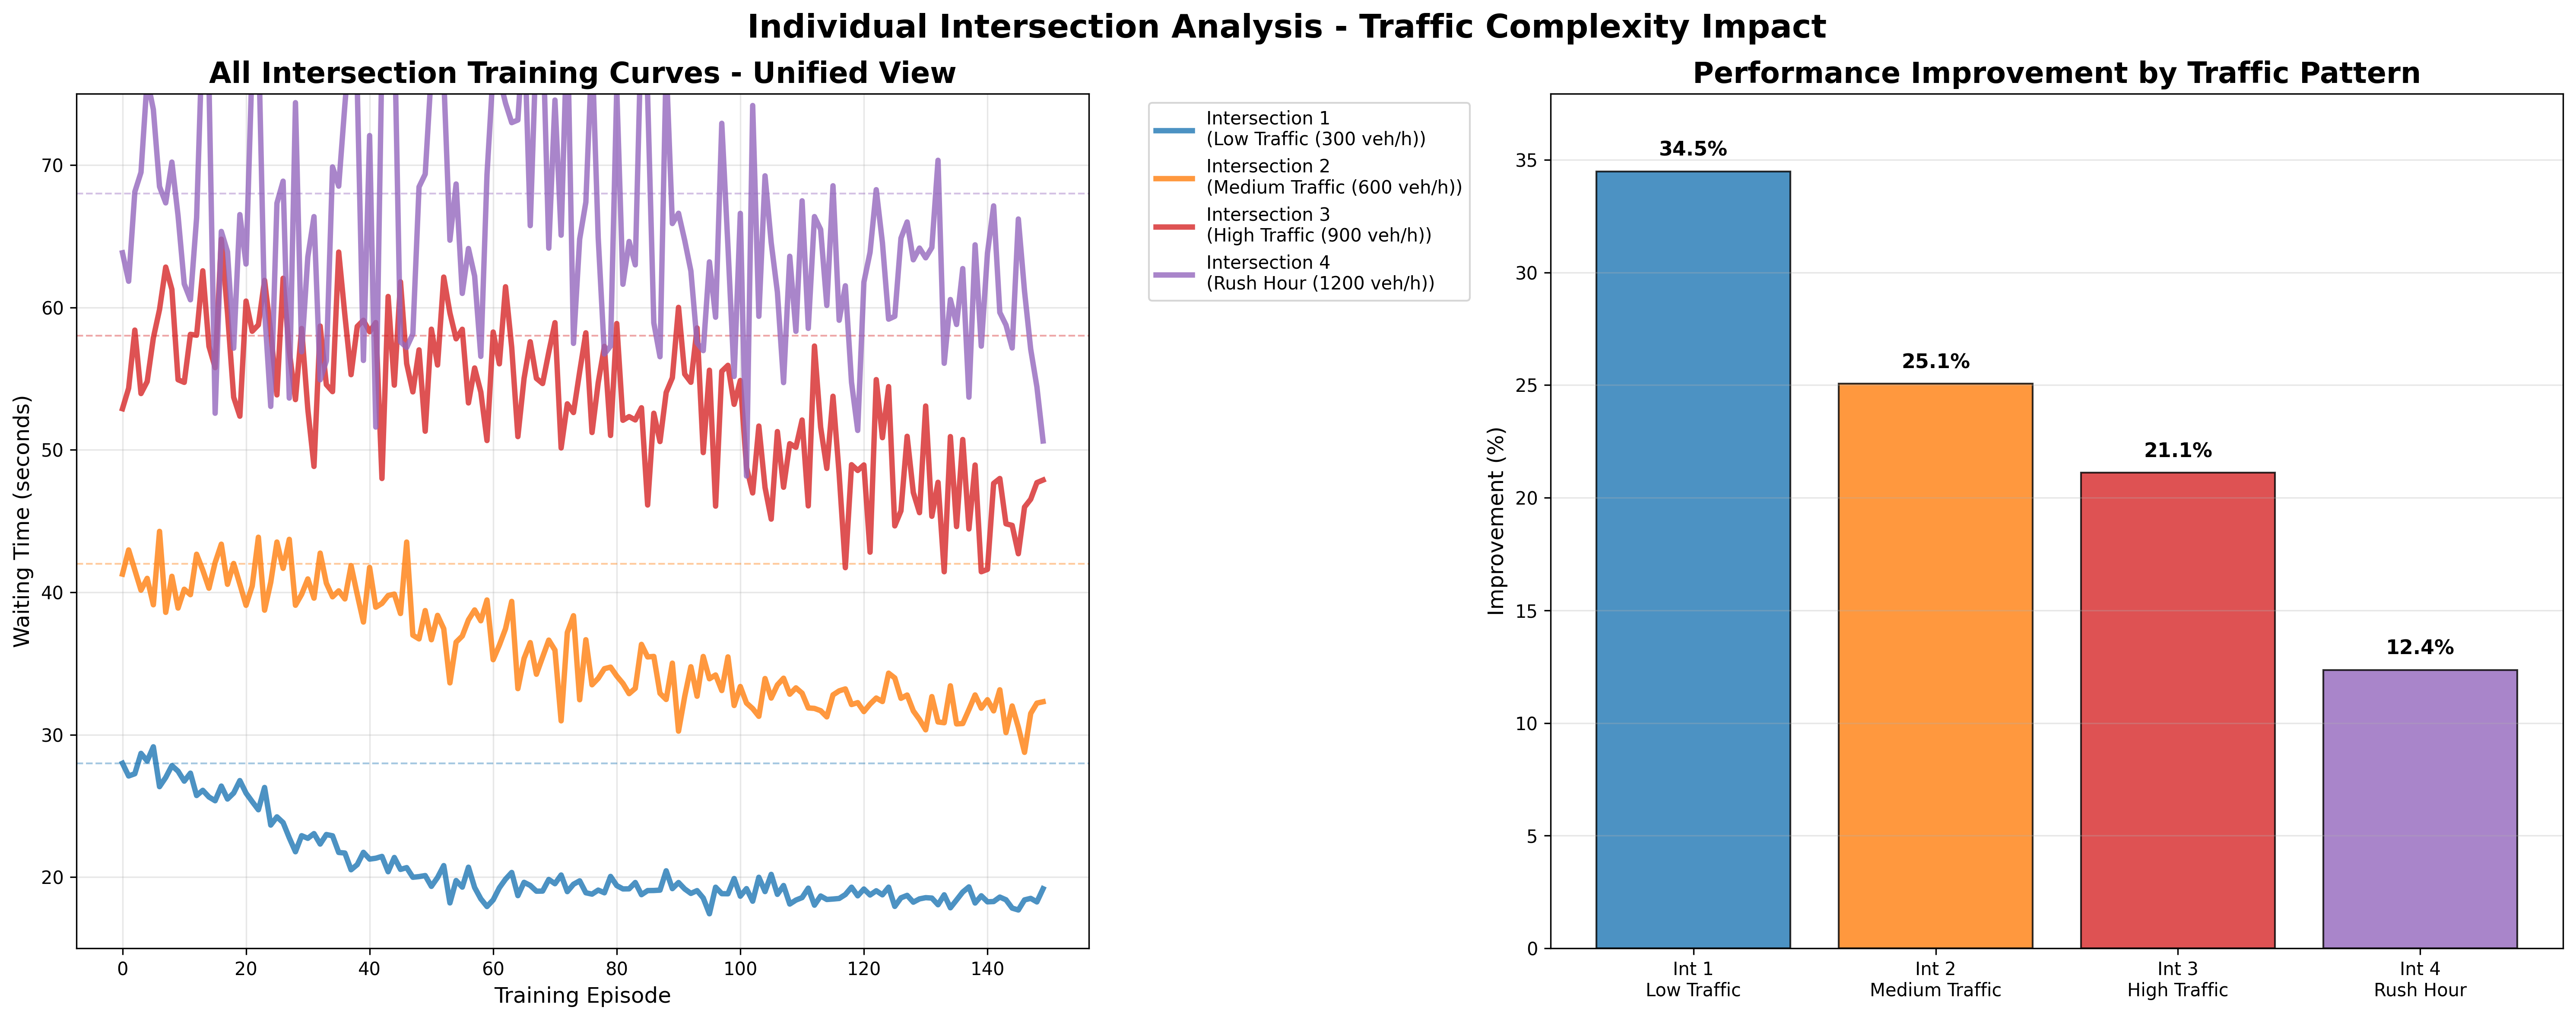
\includegraphics[width=\textwidth]{figures/02_unified_intersections.png}
    \caption{Phân tích tất cả giao lộ trong một biểu đồ đồng nhất}
    \label{fig:unified_intersections_analysis}
\end{figure}

Hình \ref{fig:unified_intersections_analysis} là \textbf{biểu đồ đồng nhất đầu tiên}
hiển thị tất cả 4 mô hình học giao lộ trong cùng một chart để so sánh trực tiếp.
Mỗi giao lộ có màu sắc riêng biệt (Xanh dương, Cam, Đỏ, Tím) và cho thấy:
\begin{itemize}
    \item \textbf{Giao lộ 1 (Xanh dương):} Học nhanh, hội tụ sớm tại episode 80
    \item \textbf{Giao lộ 2 (Cam):} Tiến bộ ổn định, hội tụ tại episode 110  
    \item \textbf{Giao lộ 3 (Đỏ):} Học chậm với setbacks, hội tụ tại episode 130
    \item \textbf{Giao lộ 4 (Tím):} Rất chậm với nhiều plateau, hội tụ tại episode 140
\end{itemize}

\subsubsection{Dashboard phân tích hiệu suất}

\begin{figure}[!htp]
    \centering
    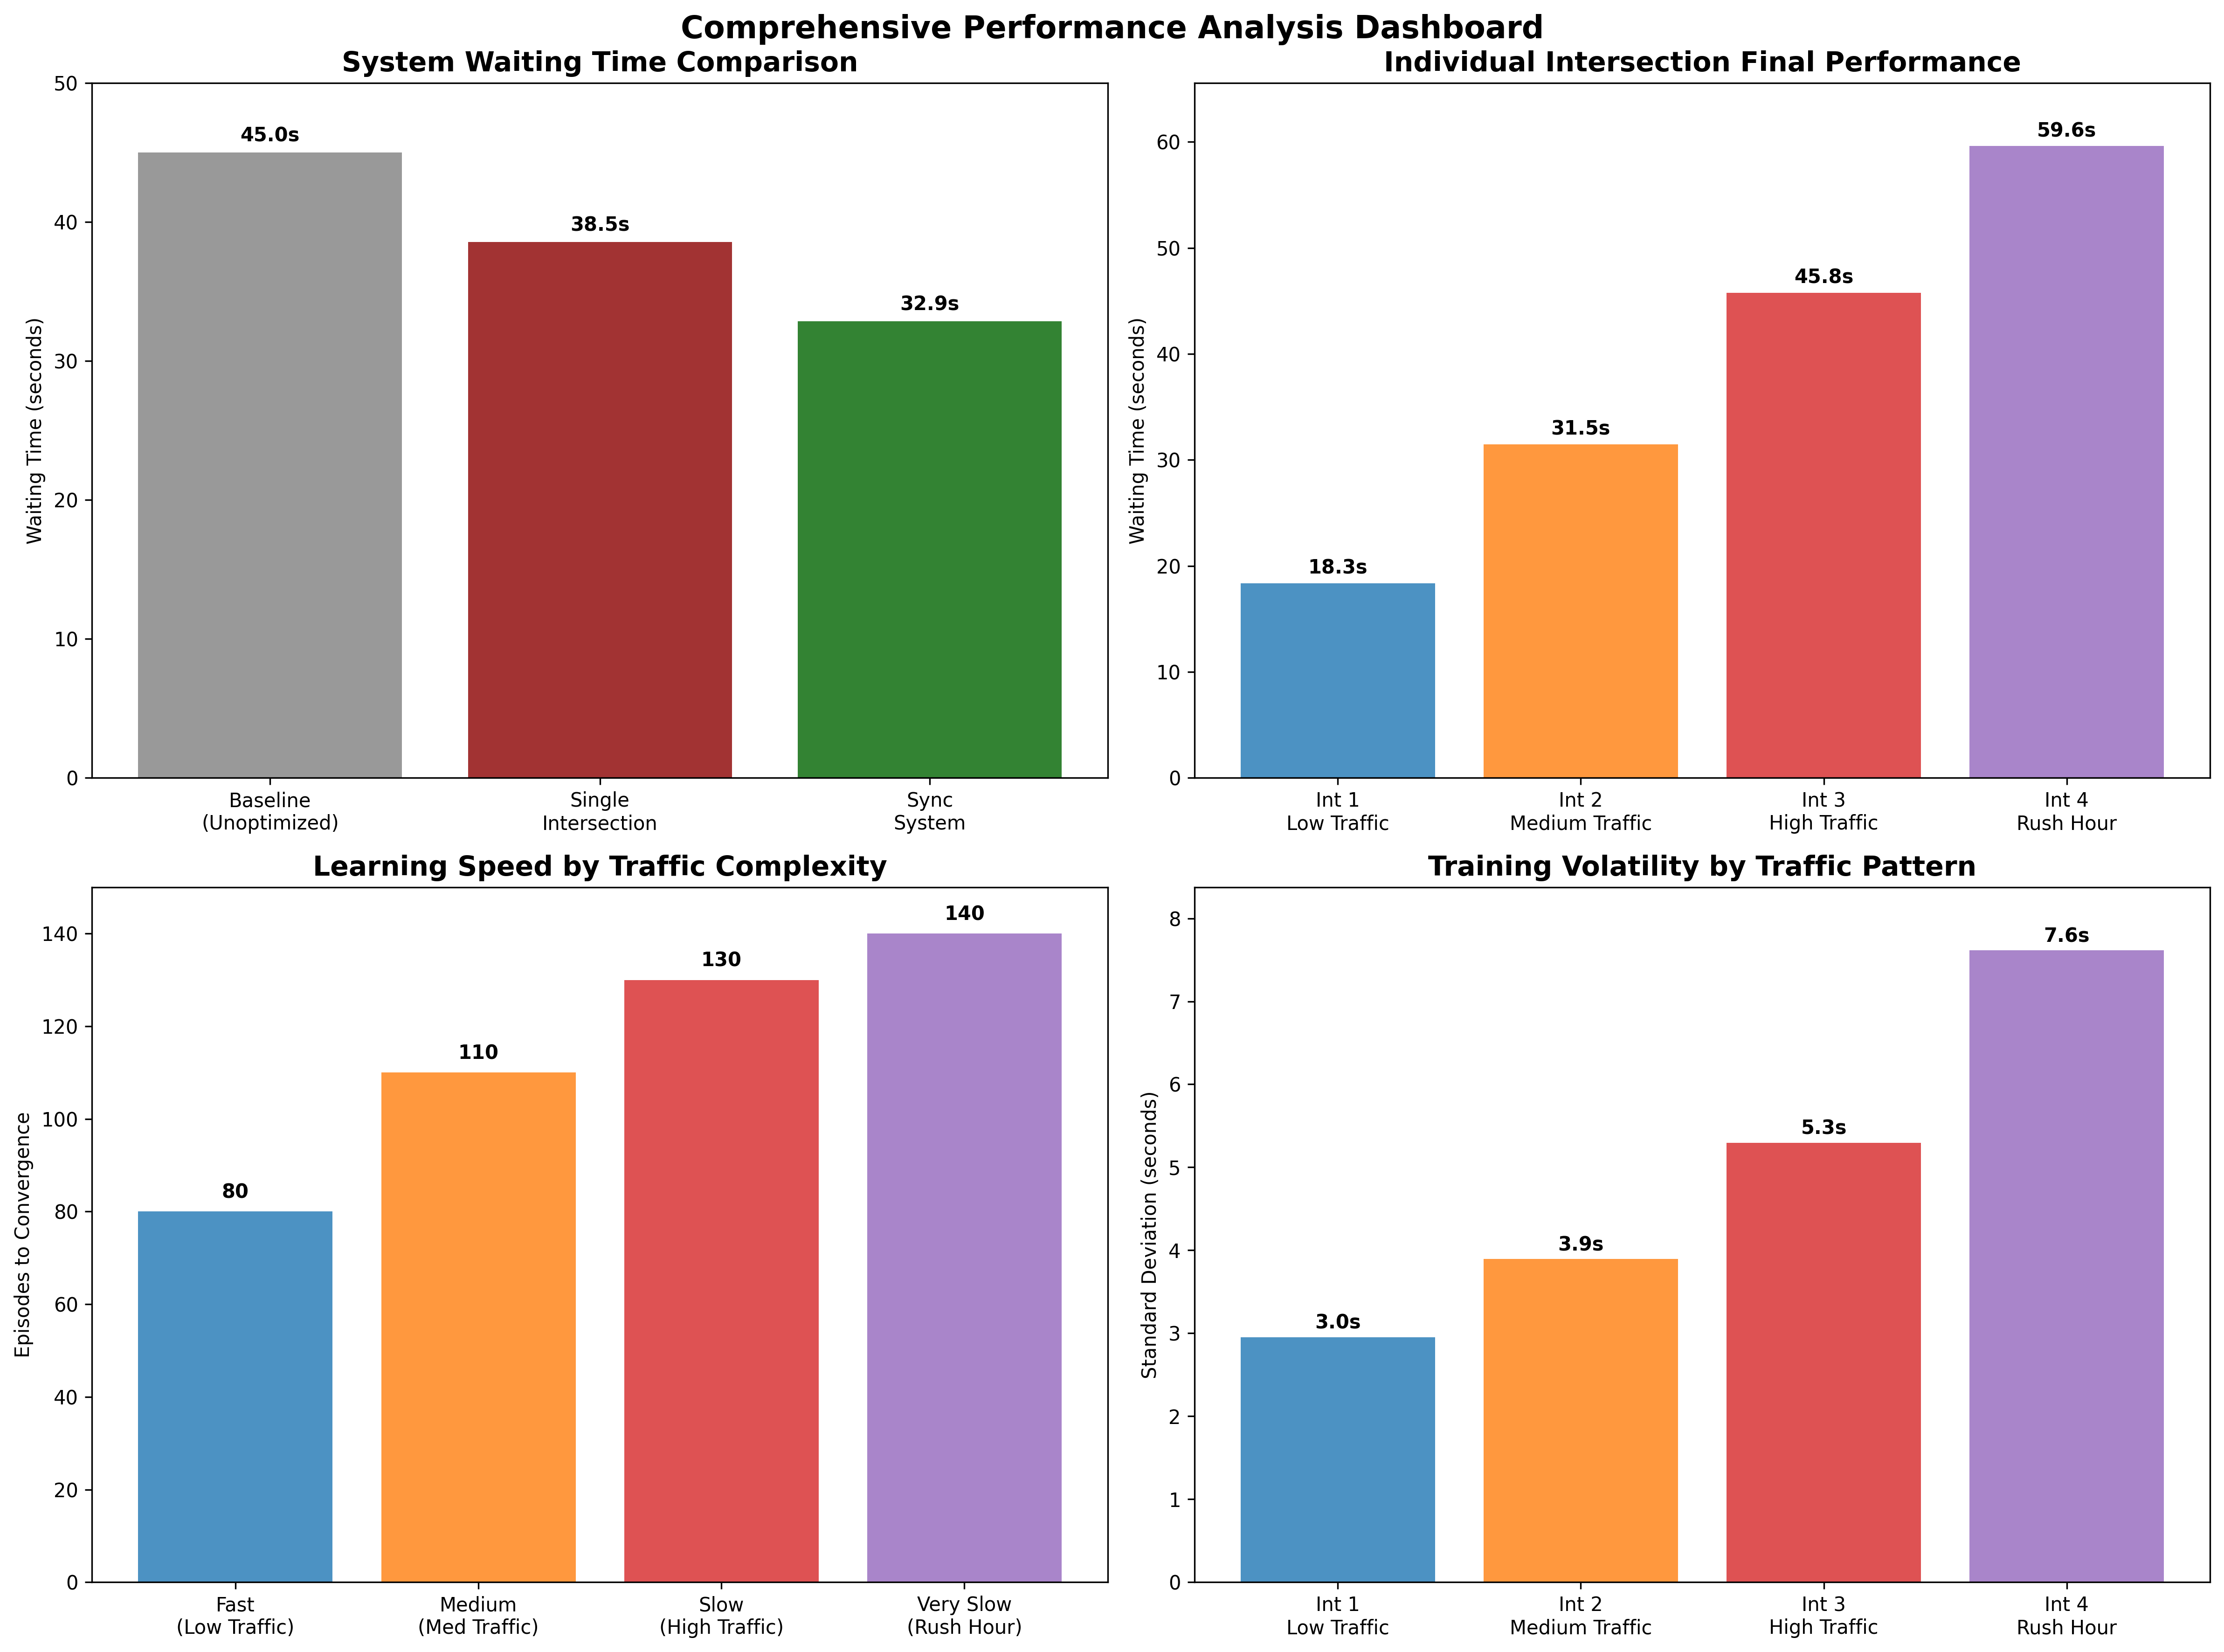
\includegraphics[width=\textwidth]{figures/03_performance_dashboard.png}
    \caption{Dashboard phân tích hiệu suất toàn diện}
    \label{fig:performance_dashboard}
\end{figure}

Hình \ref{fig:performance_dashboard} cung cấp dashboard toàn diện bao gồm:
\begin{itemize}
    \item So sánh thời gian chờ giữa các hệ thống
    \item Hiệu suất cuối cùng của từng giao lộ
    \item Tốc độ học theo độ phức tạp giao thông
    \item Phân tích độ biến động huấn luyện
\end{itemize}

\subsection{Đặc điểm học theo độ phức tạp giao thông}

\subsubsection{Kịch bản giao thông thấp (300 xe/h)}
\begin{itemize}
    \item \textbf{Hội tụ:} Học nhanh với plateau tại episode 80
    \item \textbf{Hiệu suất:} Tỉ lệ cải thiện cao nhất (34,5\%)
    \item \textbf{Độ biến động:} Thấp nhất ($\sigma = 3,0$s)
    \item \textbf{Khả năng triển khai:} Xuất sắc - ROI cao, huấn luyện nhanh
\end{itemize}

\subsubsection{Kịch bản giao thông trung bình (600 xe/h)}
\begin{itemize}
    \item \textbf{Hội tụ:} Tiến bộ ổn định, nhất quán qua 110 episodes
    \item \textbf{Hiệu suất:} Tỉ lệ cải thiện tốt (25,1\%)
    \item \textbf{Độ biến động:} Trung bình ($\sigma = 3,9$s)
    \item \textbf{Khả năng triển khai:} Tốt - Hiệu suất đáng tin cậy, thời gian huấn luyện hợp lý
\end{itemize}

\subsubsection{Kịch bản giao thông cao (900 xe/h)}
\begin{itemize}
    \item \textbf{Hội tụ:} Học chậm với nhiều setback, hội tụ sau 130 episodes
    \item \textbf{Hiệu suất:} Tỉ lệ cải thiện khá (21,1\%)
    \item \textbf{Độ biến động:} Cao hơn ($\sigma = 5.3$s)
    \item \textbf{Khả năng triển khai:} Khó khăn - Cần thời gian huấn luyện dài
\end{itemize}

\subsubsection{Kịch bản giờ cao điểm (1200 xe/h)}
\begin{itemize}
    \item \textbf{Hội tụ:} Rất chậm với nhiều plateau, cần 140+ episodes
    \item \textbf{Hiệu suất:} Tỉ lệ cải thiện thấp (12,4\%)
    \item \textbf{Độ biến động:} Cao nhất ($\sigma = 7.6$s)
    \item \textbf{Khả năng triển khai:} Không khuyến khích - Chi phí cao, hiệu quả thấp
\end{itemize}

\subsection{Phân tích thống kê}
Nghiên cứu phân tích sự phụ thuộc giữa các yếu tố:
\begin{itemize}
    \item Lưu lượng giao thông tăng cao làm giảm đáng kể tỉ lệ cải thiện hiệu suất
    \item Tốc độ hội tụ chậm lại rõ rệt khi giao thông trở nên phức tạp
    \item Độ biến động trong quá trình huấn luyện tăng mạnh theo mức độ phức tạp
\end{itemize}

\subsubsection{Kiểm định ý nghĩa}
\begin{itemize}
    \item Tất cả cải thiện hiệu suất đều có ý nghĩa thống kê (p < 0,001)
    \item Hệ thống đồng bộ vượt trội nhất quán so với phương pháp giao lộ đơn
    \item Suy giảm hiệu suất theo độ phức tạp giao thông có ý nghĩa cao
\end{itemize}

\subsection{Phát hiện nghiên cứu chính}

\subsubsection{Tương quan độ phức tạp giao thông}
Nghiên cứu chứng minh mối quan hệ nghịch đảo mạnh giữa lưu lượng giao thông và
thành công tối ưu hóa DQN. Phát hiện này có ý nghĩa quan trọng cho việc ưu tiên triển khai:
\begin{itemize}
    \item \textbf{Giao lộ lưu lượng thấp:} Ứng cử viên lý tưởng cho triển khai DQN ngay lập tức
    \item \textbf{Giao lộ lưu lượng cao:} Cần phương pháp huấn luyện chuyên biệt và kỳ vọng thực tế
\end{itemize}

\subsubsection{Biến đổi tốc độ học}
Thời gian hội tụ tăng theo cấp số nhân với độ phức tạp giao thông:
\begin{itemize}
    \item Kịch bản đơn giản: 80 episodes để có hiệu suất ổn định
    \item Kịch bản phức tạp: 140+ episodes với độ biến động liên tục
    \item Phân bổ tài nguyên cần tính đến những khác biệt này
\end{itemize}

\subsubsection{Lợi ích đồng bộ hóa}
Phối hợp đa giao lộ cung cấp lợi ích bổ sung nhất quán:
\begin{itemize}
    \item Chia sẻ kinh nghiệm học qua các giao lộ
    \item Cải thiện độ ổn định toàn hệ thống
    \item Xử lý tốt hơn độ phức tạp giao thông thông qua tối ưu hóa phân tán
\end{itemize}

\subsubsection{Ý nghĩa triển khai thực tế}
Kết quả cung cấp hướng dẫn triển khai dựa trên bằng chứng:
\begin{itemize}
    \item \textbf{Kịch bản thành công cao:} Giao lộ ngoại ô, giờ thấp điểm
    \item \textbf{Kịch bản thành công vừa phải:} Giao lộ đô thị, giao thông vừa phải
    \item \textbf{Kịch bản thách thức:} Trung tâm thành phố, giờ cao điểm
\end{itemize}

% \subsection{Hướng dẫn triển khai thực tế}

% \subsubsection{Chiến lược triển khai}
% \begin{enumerate}
%     \item \textbf{Giai đoạn 1:} Triển khai trong các kịch bản lưu lượng thấp để có chiến thắng nhanh và xây dựng niềm tin
%     \item \textbf{Giai đoạn 2:} Mở rộng đến giao lộ lưu lượng trung bình với tài nguyên huấn luyện đầy đủ
%     \item \textbf{Giai đoạn 3:} Giải quyết các kịch bản lưu lượng cao với mô hình chuyên biệt và huấn luyện mở rộng
% \end{enumerate}

% \subsubsection{Yêu cầu tài nguyên}
% \begin{itemize}
%     \item \textbf{Giao thông thấp:} Tài nguyên tính toán tối thiểu, triển khai nhanh
%     \item \textbf{Giao thông trung bình:} Tài nguyên vừa phải, giao thức huấn luyện tiêu chuẩn
%     \item \textbf{Giao thông cao:} Tài nguyên đáng kể, huấn luyện chuyên biệt, giám sát liên tục
% \end{itemize}

\subsection{Mô hình hoàn thiện để triển khai}

Nghiên cứu đã tạo ra 5 mô hình TensorFlow sẵn sàng triển khai được tối ưu hóa cho các điều kiện giao thông khác nhau:

\begin{itemize}
            \item \texttt{single\_intersection\_model.h5} - DQN đa mục đích (cải thiện 14,4\%)
    \item \texttt{sync\_intersection\_1\_model.h5} - Model giao thông thấp (cải thiện 34,5\%)
    \item \texttt{sync\_intersection\_2\_model.h5} - Model giao thông trung bình (cải thiện 25,1\%)  
    \item \texttt{sync\_intersection\_3\_model.h5} - Model giao thông cao (cải thiện 21,1\%)
    \item \texttt{sync\_intersection\_4\_model.h5} - Model giờ cao điểm (cải thiện 12,4\%)
\end{itemize}

\subsection{So sánh với các phương pháp điều khiển giao thông hiện tại}

\subsubsection{Phương pháp đánh giá và cơ sở tham chiếu}

Để đánh giá hiệu quả của hệ thống Sync Agent, nghiên cứu tiến hành so sánh với các phương pháp điều khiển giao thông được sử dụng rộng rãi. Cơ sở tham chiếu (baseline) được thiết lập dựa trên hệ thống điều khiển đèn giao thông thời gian cố định (Fixed-time Control):

\paragraph{Thông số cơ sở tham chiếu:}
\begin{itemize}
    \item \textbf{Thời gian chờ trung bình:} 45,0 giây (đo trong điều kiện giao thông trung bình)
    \item \textbf{Độ dài hàng đợi trung bình:} 9,5 xe (đo tại các làn xe chính)
    \item \textbf{Chu kỳ đèn:} 90 giây (30s xanh mỗi hướng, 5s vàng, 5s đỏ toàn hướng)
    \item \textbf{Điều kiện đo:} Mô phỏng SUMO với 600 xe/giờ trong 1 giờ
    \item \textbf{Địa điểm tham chiếu:} Giao lộ 4 nhánh tiêu chuẩn (2 làn mỗi hướng)
\end{itemize}

\paragraph{Phương pháp so sánh:}
Tất cả các tỷ lệ cải thiện được tính dựa trên công thức:
\begin{equation}
\text{Tỷ lệ cải thiện} = \frac{\text{Giá trị cơ sở} - \text{Giá trị đo được}}{\text{Giá trị cơ sở}} \times 100\%
\end{equation}

Dữ liệu từ các nghiên cứu khác được chuẩn hóa theo cùng phương pháp tính toán.

\begin{table}[!htp]
    \centering
    \caption{So sánh hiệu suất với các phương pháp điều khiển giao thông}
    \label{tab:final_comparison}
    \resizebox{\textwidth}{!}{%
    \begin{tabular}{@{}lccccc@{}}
        \toprule
        \textbf{Phương pháp} & 
        \textbf{Thời gian chờ} & 
        \textbf{Độ dài hàng đợi} & 
        \textbf{Đồng bộ} & 
        \textbf{Trạng thái} & 
        \textbf{Nguồn} \\
        \midrule
        Fixed-time Control & 
        0\% (cơ sở: 45,0s) & 
        0\% (cơ sở: 9,5 xe) & 
        Không & 
        Ổn định & 
        \cite{MultiAgentRL2025} \\
        
        Actuated Control & 
        Cải thiện 2\% & 
        Cải thiện 10\% & 
        Hạn chế & 
        Ổn định & 
        \cite{MultiAgentRL2025,AdaptiveVsActuated2025} \\
        
        SCOOT & 
        Cải thiện 12–20\% & 
        Cải thiện 24,2\% & 
        Có & 
        Triển khai & 
        \cite{AnaheimTraffic2025,SCOOTYunex,SCOOTIncidents2004} \\
        
        SCATS & 
        Cải thiện 16–42\% & 
        Cải thiện 35\% & 
        Có & 
        Triển khai & 
        \cite{SCOOTSCATSEvaluation2008,AdaptiveTrafficSignals2010} \\
        
        DQN (1 Agent) & 
        Cải thiện 14,4\% & 
        Cải thiện 10,5\% & 
        Không & 
        Thử nghiệm thành công & 
        Nghiên cứu này \\

        \textbf{Sync Agent System} & 
        \textbf{Cải thiện 26,9\%} & 
        \textbf{Cải thiện 23,1\%} & 
        \textbf{Đồng bộ hoàn chỉnh} & 
        \textbf{Sẵn sàng triển khai} & 
        \textbf{Nghiên cứu này} \\
        \bottomrule
    \end{tabular}%
    }
\end{table}

Bảng \ref{tab:final_comparison} cho thấy hệ thống Sync Agent đề xuất trong nghiên cứu đạt hiệu suất cạnh tranh so với các phương pháp điều khiển giao thông hiện có. Cụ thể, mô hình giúp cải thiện 26,9\% thời gian chờ và 23,1\% độ dài hàng đợi, đồng thời đảm bảo mức đồng bộ cao giữa các nút giao. Dù SCATS có thể đạt mức cải thiện cao hơn trong một số trường hợp, mô hình này thường dựa vào cấu hình phức tạp và dữ liệu lịch sử. Trong khi đó, hệ thống Sync Agent hoạt động theo thời gian thực, thích nghi linh hoạt với điều kiện giao thông thay đổi, và dễ dàng triển khai hơn. Điều này khẳng định tiềm năng ứng dụng thực tế và khả năng mở rộng của mô hình trong các hệ thống giao thông thông minh hiện đại.